\chapter{Syntactic phenomena}

In this chapter we apply the tools of the o/el framework to a variety of syntactic phenomena, such as ellipsis, anaphora, wh-expressions, and island patterns.\footnote{These phenomena are of course very complicated and hence the treatments presented here are necessarily incomplete. The goal is to illustrate the general applicability of the o/el framework, rather than establish a definitive understanding of the phenomena. Moreover, the analyses conducted are of coherence intuitions that are my own, and without further empirical work there is no guarantee that my intuitions correspond to intuitions which other speakers may have. I can only hope that there is no great disparity between my intutitions and those which are normal among native speakers. The reliance I have on \textit{Al} and \textit{Bo}, \textit{drinks} and \textit{eats}, and \textit{coffee}, \textit{tea}, and \textit{granola}, is a potential problem as well, to the extent that proper names, simple/habitual tense-aspect ambiguity, and mass nouns could lead to abnormal coherence intuitions in various contexts.} We reject various object-metaphor conceptualizations of these phenomena—movement, copying, deletion, feature matching, etc.—but may use some terminology that evokes them for convenience. In most cases we pursue analyses of the phenomena from the perspective of production. However, we make the assumption that producers obtain a coherent trajectory prior to selective production; hence we conflate producer and interpreter to some degree by conjecturing that utterance coherence is required for production. One can envision a parallel approach which pursues analyses from the perspective of interpretation; but due to our emphasis on potentially reiterative trajectories (i.e. utterance coherence), production-based and interpretation-based analyses may not be substantively different. 

\section{Ellipsis}

From a conventional perspective, ellipsis is commonly conceptualized as a phenomenon in which objects are “deleted” from a structure, often when those same objects are present elsewhere in the structure \citep{Merchant2001,Merchant2005,Merchant2013}). For example, consider the utterance below. We might expect \textit{Al drank} to be selected again in the second clause:

\ea
  {Al drank coffee first and} (Al drank) \textit{tea second}
\z

  The elided words in this example, and in general, are not necessarily a constituent in the conventional view. Although we can imagine any sequence of words being elided, not all possible ellipses are coherent. Here we construct an o/el understanding of ellipsis and develop analyses of why some ellipses are coherent and others are not.

\subsection{Motoric vs. syntactic accounts}

With o/el conceptual tools, there are two types of accounts of ellipsis, one motoric and the syntactic. This also happens to be the case for conventional approaches. For several reasons the syntactic account is preferable, but lets consider both approaches for the sake of argument. 

  For the motoric account, we imagine that cs-system trajectories are canonical: the cs-systems associated with elided words are in fact selected, but gm-systems in the gm-domains of these cs-systems are not selected. This account is “motoric” because ellipsis is understood as the non-selection of gestural-motoric systems; it can be construed as m-gating applied to particular systems. In contrast, for the syntactic account, we imagine that cs-systems associated with the elided words are not selected, and hence the cs-trajectory is non-canonical.

  To see how motoric and syntactic accounts differ, lets consider the gapping ellipsis \textit{Al drank coffee first and tea second}, shown below. In both accounts, [Al]\{N\} and [drank]\{V\} are promoted to selection and demoted, prior to epoch (e1). For the motoric account, at a later epoch (e2), [Al]\{N\} and [drank]\{V\} are once again promoted to selection. However, the gm-domains associated with these cs-systems are not re-excited (or alternatively, are excited but do not reach selection-level). In contrast, in the syntactic account we hypothesize that [Al]\{N\} and [drank]\{V\} remain excited during the later epoch (e2) but are not re-promoted to selection level. 

  
\begin{figure}
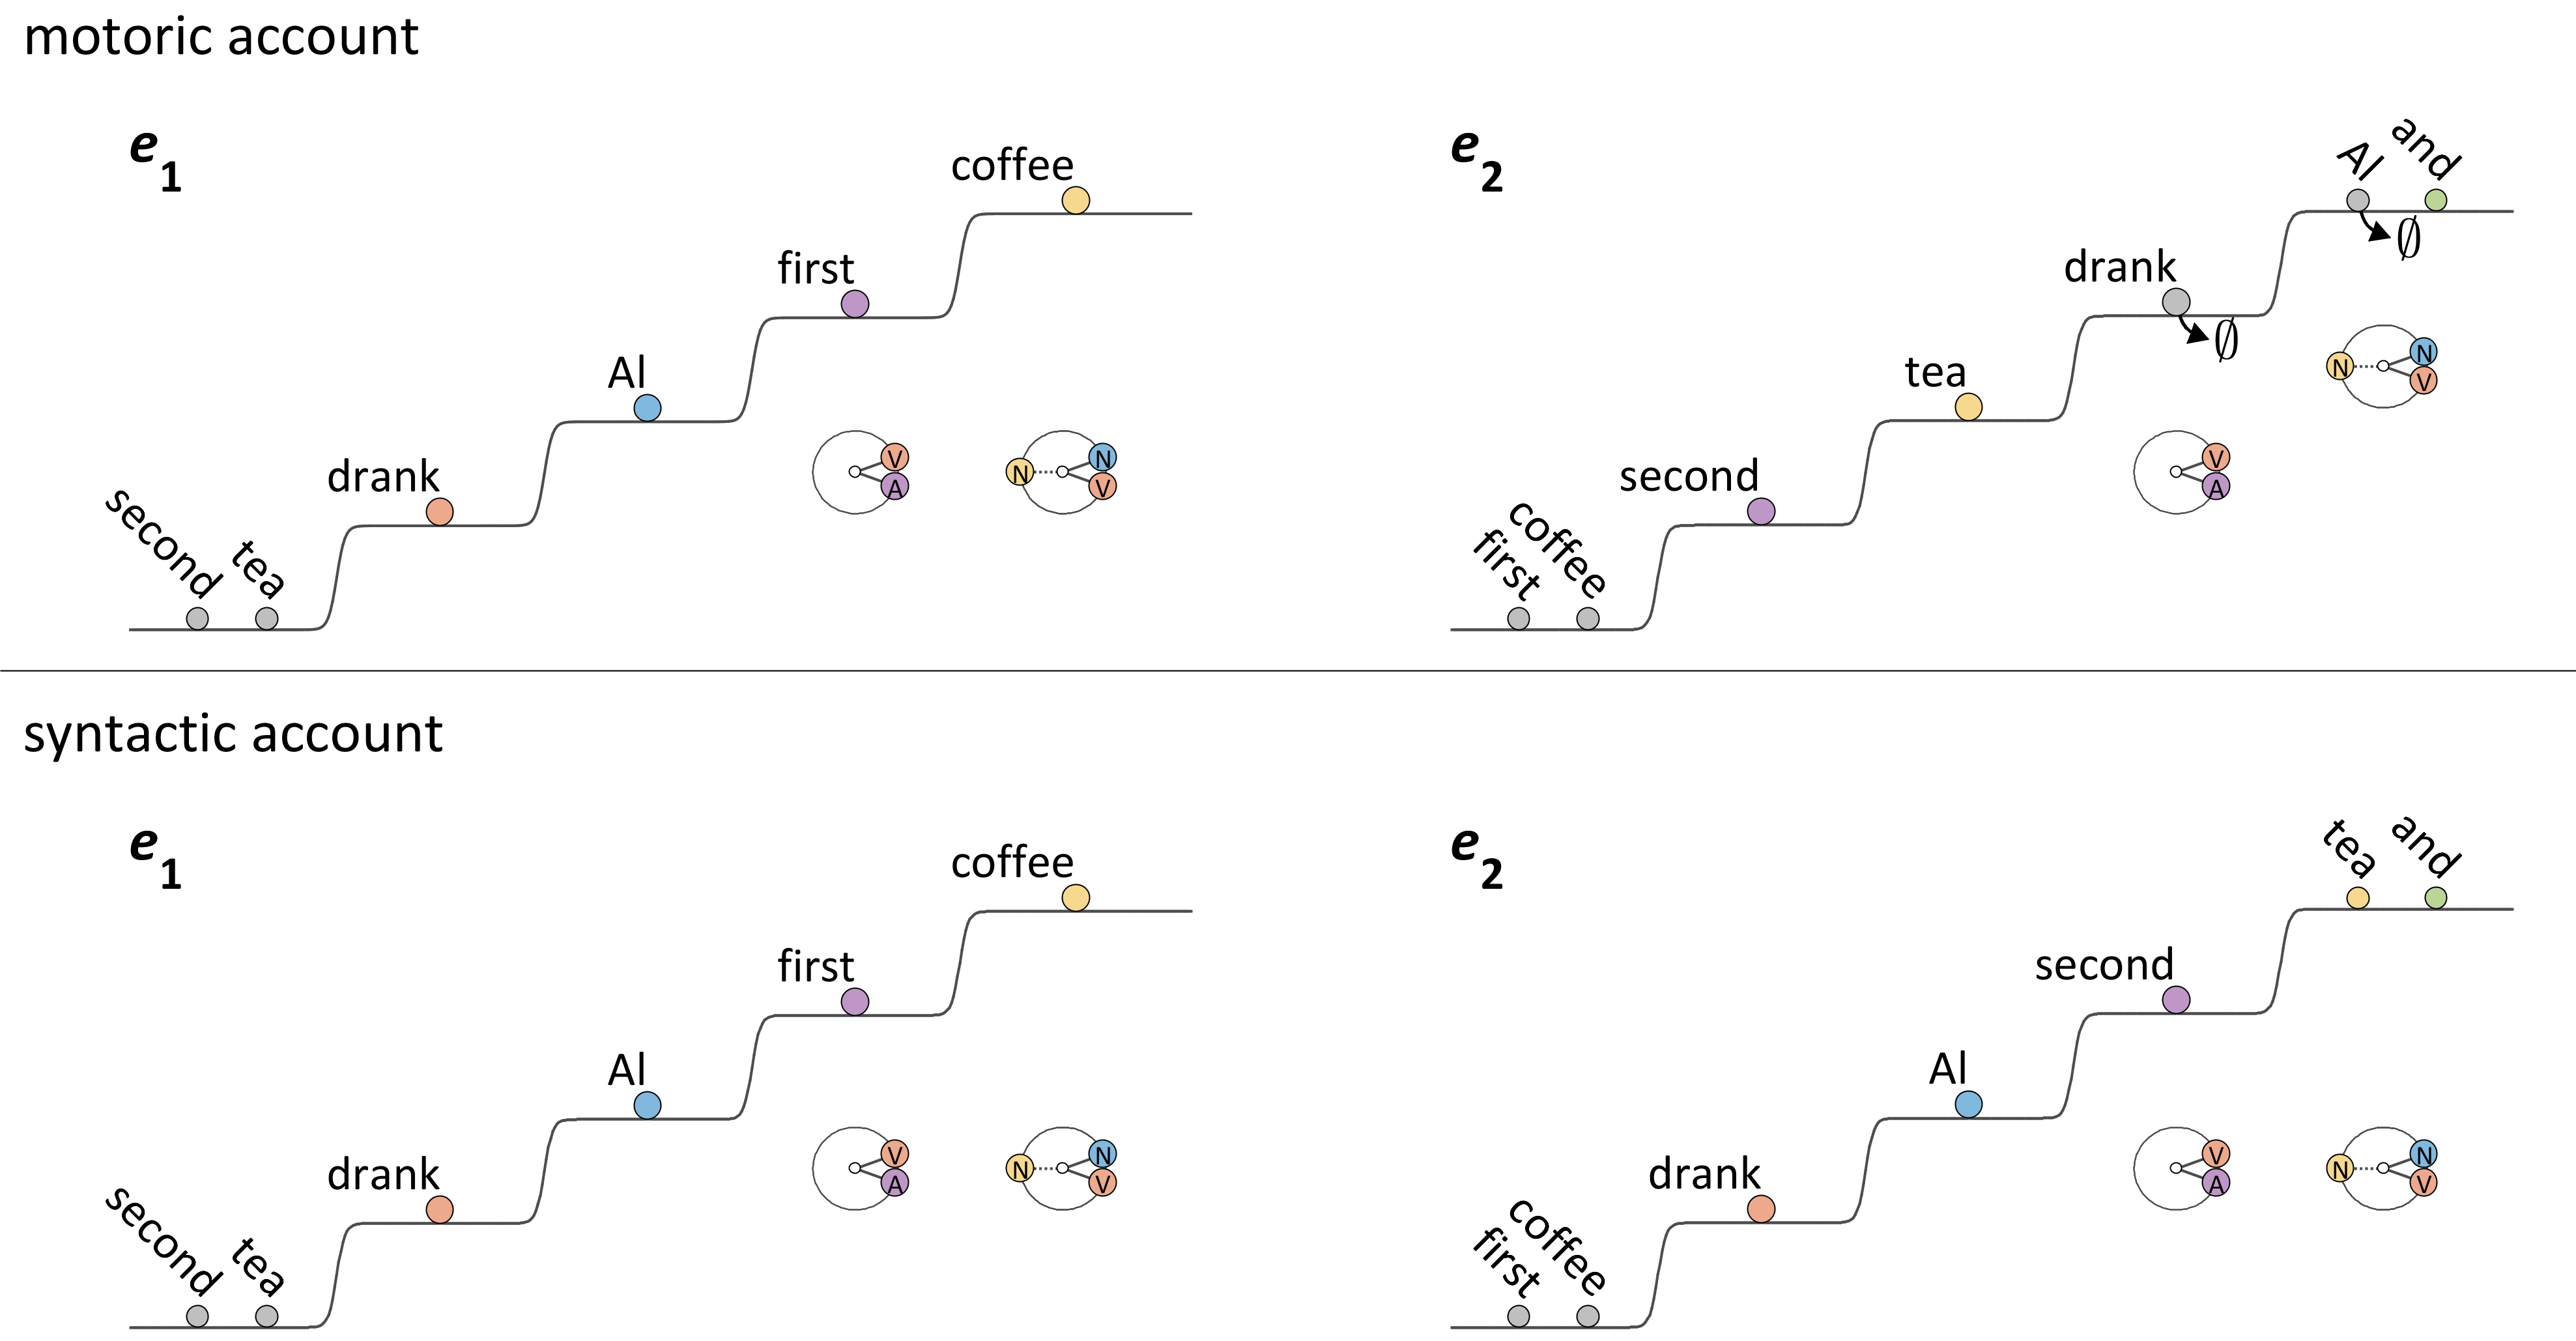
\includegraphics[width=\textwidth]{figures/Tilsen-img145.png}
\caption{\missingcaption}
\label{fig:7:1}
\end{figure}
 

  In both approaches, [Al]\{N\} and [drank]\{V\} persist in an above ground state and give rise to {\textbar}Al drank tea{\textbar} and {\textbar}drank second{\textbar} φ configurations. The two approaches differ regarding whether the ellipsis is a non-canonical gm- trajectory (the motoric account) or non-canonical cs-trajectory (the syntactic account). The question is, do both possible types of ellipsis occur, or should we always prefer just one in our analyses? Readers may recognize in the following example the old disagreement about whether non-constituent coordination is really coordination of constituents in deep structure, with the apparent non-constituent coordination being a consequence of surface deletion \citep{DalrympleEtAl1991,Merchant2001,SagEtAl1985}: 

  \ea
{Al drank coffee first and} (\textit{Al drank} [F0E0?] Ø) \textit{tea second}
\z

  One of the motivations for positing such deep structure is to serve semantic interpretation. The conventional paradigm requires objects to be “present” \textit{somewhere}, so that meaning can be determined from structure. In the o/el framework, relational meaning experiences arise from attentionally focused (excited) cs-system φ configurations, and hence we require the relevant systems to be above ground and φ-coupled. We do not, however, require selection-level excitation for relational meaning, and this allows for a syntactic account in which systems can persist in an excited state and support φ configurational meaning, without being selected. 

\subsection{Ellipsis in coordinative vs. subordinative reorganizations}

The syntactic account of ellipsis relies on the distinctions between canonical vs. ungrounding promotion and canonical vs. grounding demotion, developed earlier in our analysis of canonical and selective reorganization. One useful application of these distinctions is to account for coherence intuitions of ellipses in coordinate vs. subordinate clause structures. Consider the following coherence contrast:

\ea
   \ea[]{Al drank coffee, and Bo tea}
\ex[*/?]{Al drank coffee, if Bo tea}
\z
\z

  Why is ellipsis of the \{V\} system less coherent when in a subordinate clause than in a coordinate clause? The reduced coherence suggests that [drink]\{V\} cannot as readily form a φ configuration with [Bo] and [tea]. Because of this we infer that [drink]\{V\} is more likely to be grounded in the epochs during which [Bo] and [tea] are excited. To account for the contrast, we hypothesize a distinction between reorganizations associated with coordinate and subordinate clauses: coordinating reorganizations allow for cs-systems to remain excited, subordinating reorganizations necessarily ground all previously excited systems. 

  Specifically, in a coordinative reorganization, lexical cs-systems from the previous epoch can remain excited, if those systems do not interfere with a cs-system promoted from ground in the coordinative reorganization. Hence in the coordination trajectory below, [drank]\{V\} remains excited after Ê\textsubscript{4}, while [Al] and [coffee] are grounded. The reason [Al]\{N\} and [coffee]\{N\} are grounded in this reorganization is because they interfere with cs-systems [Bo]\{N\} and [tea]\{N\}. In contrast, Ê\textsubscript{4} in the subordinative reorganization grounds all cs-systems, including [drank]\{V\}. Hence [Bo] and [tea] cannot participate in a φ configuration with a \{V\} in (e4), thereby inducing non-coherence. Note that our analysis constructs just one [drink]\{V\} system, but we might also allow for an analysis in which [drink] and \{V\} systems are differentiated in parallel. Parallel c-/s- differentiations of this sort can be viewed as states which induce ellipsis, i.e. the non-selection of cs-systems which experience parallel c-/s- differentiation.

  
\begin{figure}
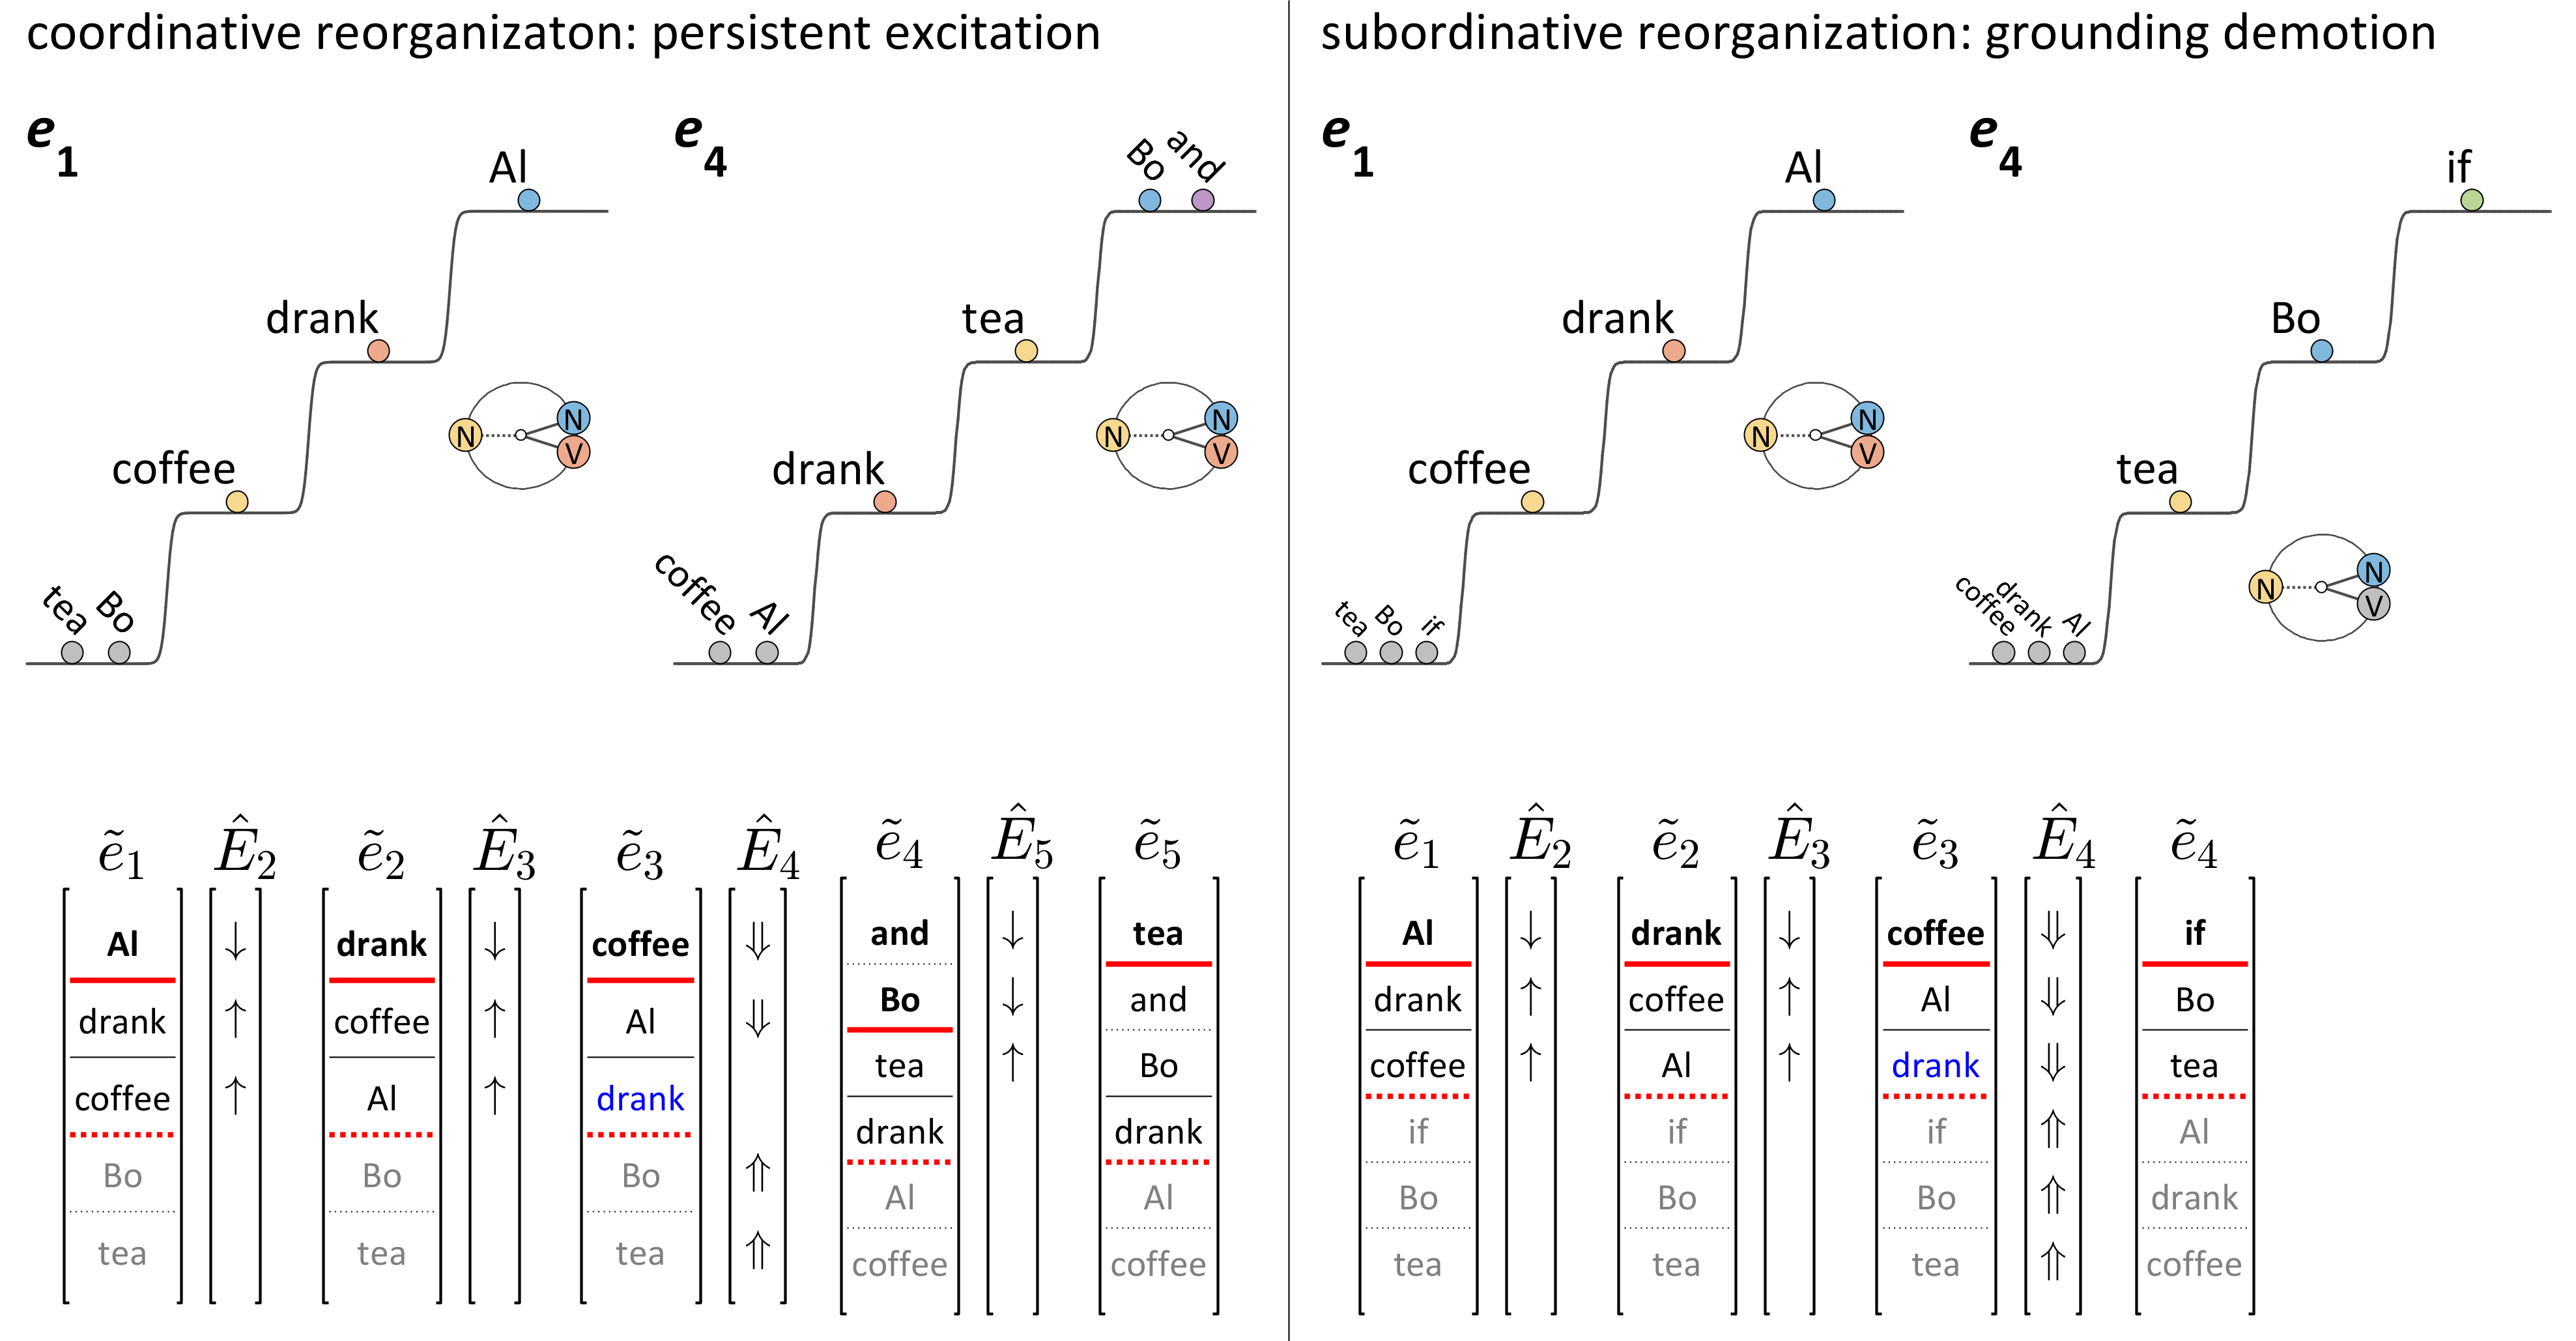
\includegraphics[width=\textwidth]{figures/Tilsen-img146.png}
\caption{\missingcaption}
\label{fig:7:2}
\end{figure}
 

  One aspect of the above analysis worth emphasizing is that we think of the coordinating conjunctions such as [and]\{\textsc{conj}\}, [but]\{\textsc{conj}\}, and [or]\{\textsc{conj}\} as systems which are specifically associated with promotion from ground in a coordinative reorganization. Hence when [Bo]\{N\} and [tea]\{N\} are promoted from ground in reorganization Ê\textsubscript{4}, we imagine [and]\{\textsc{conj}\} to be activated and excited. In contrast, we analyze subordinators such as [if]\{\textsc{sub}\}, [when]\{\textsc{sub}\}, etc. as cs-systems which are activated in parallel with grounded cs-systems. This suggests a fundamental difference between coordination and subordination such that subordinators correspond to systems which are in φ configurations with other systems (usually \{V\}), while coordinators are manifestations of ungrounding promotion operations.

  Furthermore, the reader should note that the non-coherence intuitions motivating the above analysis can be diminished if one “tries hard” to evoke the {\textbar}Bo drank tea{\textbar} configuration in the subordinative reorganization. Perhaps this effortful adjustment adapts the subordinative reorganization to be more like a coordinative one, i.e. one which maintains [drank]\{V\} above ground. Thus we infer that in the typical subordinative reorganization trajectory, excitation of a subordinate clause grounds other systems, but this operation can be overridden via a mechanism which maintains the relevant system in an excited state. This effortful excitation is a potential source of variability in coherence intuitions of ellipses (see \citealt{FrazierClifton2005,Phillips2003,PhillipsParker2014} for examples of empirical variability). 

  The o/el conception of ellipsis avoids any concept of deletion or omission of objects in a structure. Ellipsis corresponds to trajectory in which some cs-system(s) are not selected yet remain sufficiently excited to participate in an attended φ configuration. Because subordinative reorganizations ground previously excited systems, ellipsis in a subordinate clause is not coherent. There are, however, circumstances when previously grounded systems can be promoted from ground and thus participate in the φ configuration of the subordinate clause. 

  One such circumstance involves the presence of an auxiliary s-system \{\textsc{aux}\} in both the main and subordinate clauses. Consider the patterns in the {\tablebelow}. Contrary to expectation, we observe that ellipsis in a subordinate clause is coherent, but only when an auxiliary verb is present in the subordinate clause, as in the pseudogapping and VP-ellipsis patterns (\citealt{Johnson2001,Johnson2009,Merchant2001}):

\begin{table}
\begin{tabularx}{\textwidth}{XX}
\lsptoprule
\textbf{gapping} & \textbf{stripping}\\
\midrule 

\textit{Al will drink coffee, and Bo tea}

*\textit{Al will drink coffee, if Bo tea} & \textit{Al will drink coffee, and Bo too.}

\textit{*Al will drink coffee, if Bo too.}  \\
\tablevspace

\textbf{pseudogapping} & \textbf{VP-ellipsis}\\
\midrule 
\textit{Al will drink coffee, and Bo will tea.}

\textit{Al will drink coffee, if Bo will tea.} & \textit{Al will drink coffee, and Bo will (too).}

\textit{Al will drink coffee, if Bo will (too).}\\
\lspbottomrule
\end{tabularx}
\caption{\missingcaption}\label{tab:7:1}
\end{table}
  The salient difference between gapping/stripping and pseudogapping/VP-ellipsis is the excitation of an \{\textsc{aux}\} system in the subordinate clause. This suggests that there is a mechanism for re-exciting a previously grounded cs-system, when that cs-system is coupled to another highly excited system. We call this \textit{assisted persistence}. Hence we envision in the pseudogapping example (B) below that promotion of \{\textsc{aux}\}[will] by Ê\textsubscript{5} allows for \{V\}[drink] to remain above-ground (i.e. the demotion of \{V\} is non-grounding). This allows for a coherent {\textbar}Bo drink tea{\textbar} φ configuration. The assisted persistence mechanism may be related to the observation that [will]\{\textsc{aux}\} and [drink]\{V\} could be analyzed as differentiated cs-systems, which are strongly coupled in association with both clauses. Sentences with non-identical auxiliaries such as \textit{Al will drink coffee, and Bo did tea} are much less coherent.

  
\begin{figure}
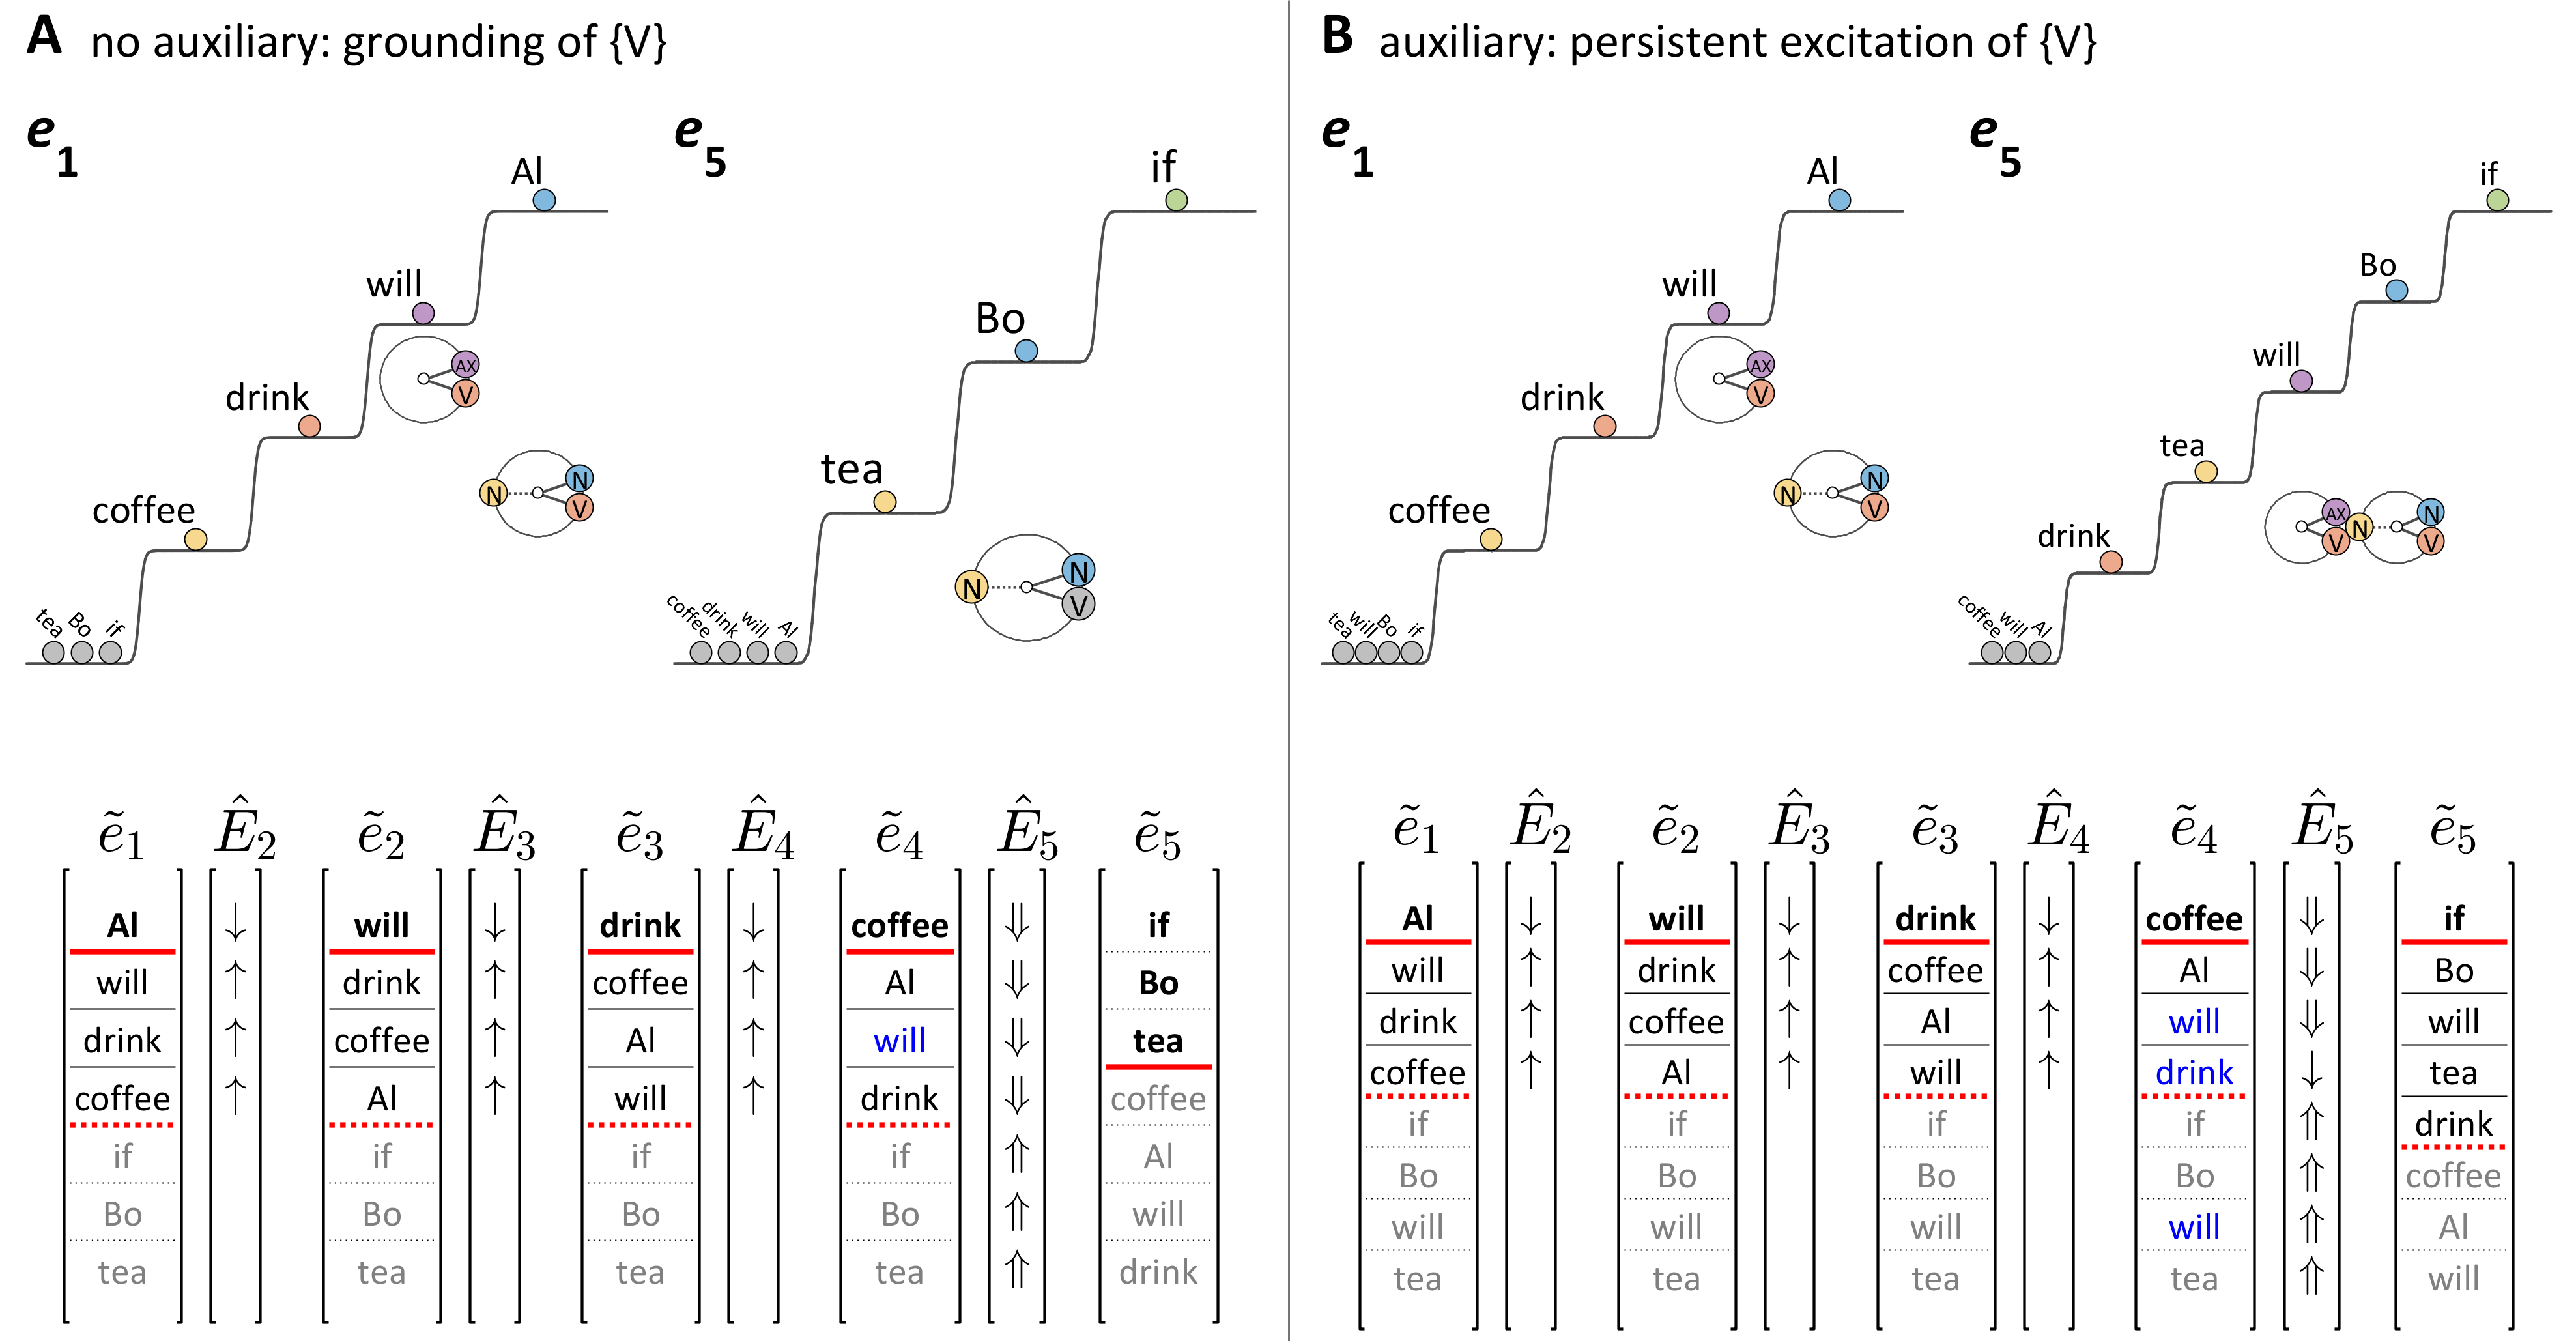
\includegraphics[width=\textwidth]{figures/Tilsen-img147.png}
\caption{\missingcaption}
\label{fig:7:3}
\end{figure}
 

  The assisted persistence mechanism is highly constrained. The examples below show that \{\textsc{aux}\} can allow \{V\} or both \{V\} and \{-N\} to persist, but cannot allow \{-N\} to persist in the absence of \{V\}, and cannot allow \{+N\} to persist above ground in any circumstances. This suggests that relative e-organization is a factor in assisted persistence and that coherence intuitions will differ in languages with different fixed word orders. 

  Another interesting aspect of the phenomenon is the influence of gm-domain identity. When \{\textsc{aux}\} selection is associated with a contracted gm-system in the subordinate clause, the elision trajectory is less coherent: 

\ea[?]{Al’ll drink coffee, if Bo’ll tea.}      \textsuperscript{?}\textit{Al’d drink coffee, if Bo’d (tea).}
\z

\ea[?]{Al will drink coffee, if Bo’ll tea.}    \textsuperscript{?}\textit{Al would drink coffee, if Bo’d (tea).}
\z

\ea{Al’ll drink coffee, if Bo will (tea).}    \textit{Al’d drink coffee, if Bo would (tea).}
\z

  These patterns might suggest that gm-excitation plays a role in the assisted persistence mechanism, but there is an alternative interpretation. Note that a key difference in cs-organization between contracted and uncontracted forms of the auxiliary is whether \{\textsc{aux}\} occupies a level of its own or is co-selected with other systems. As exemplified below, when [will]\{\textsc{aux}\} is selected independently from other lexical systems (A), [drink]\{V\} can persist in an excited state in the reorganization Ê\textsubscript{5}. However, when [will]\{\textsc{aux}\} is co-selected with [Al]\{N\} as in (B), the reorganization grounds [drink]\{V\}.

  
\begin{figure}
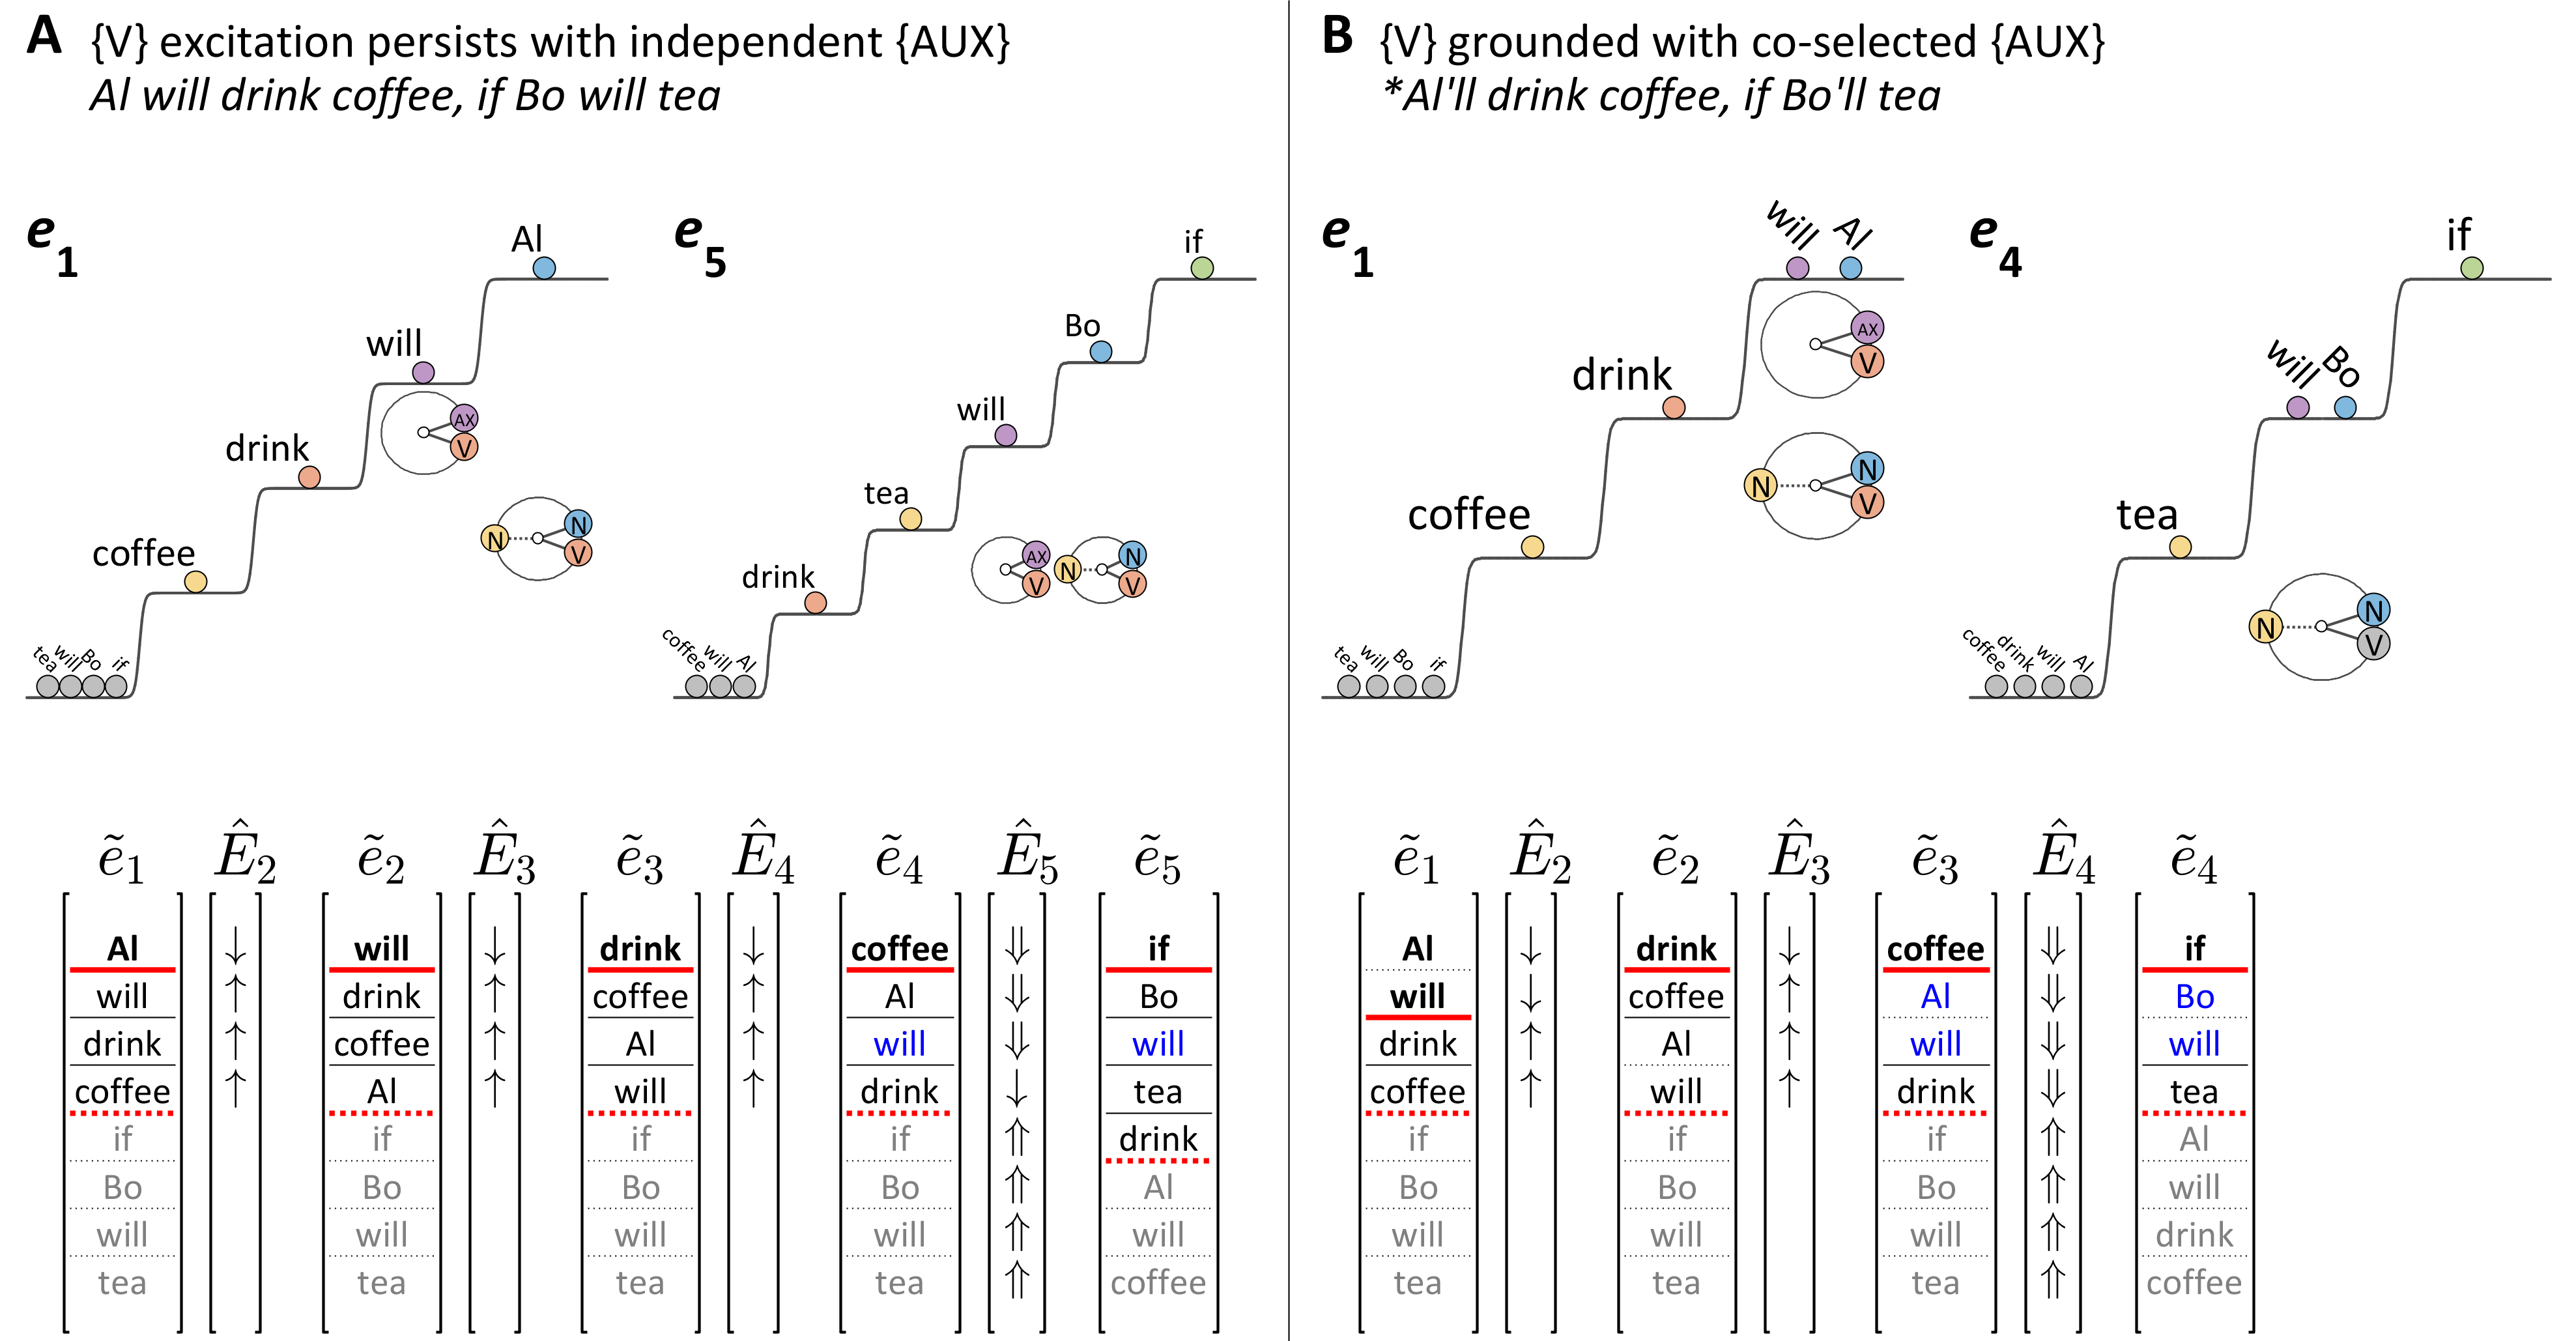
\includegraphics[width=\textwidth]{figures/Tilsen-img148.png}
\caption{\missingcaption}
\label{fig:7:4}
\end{figure}
 

  Other types of s-systems than \{\textsc{aux}\} can assist the persistence of cs-systems. Consider the complement clause elisions below. As expected, the elision is more coherent in the coordinated clause than the subordinated one. However, the selection of the nonfinite clause s-system [to]\{\textsc{fin}\} seems to facilitate a coherent interpretation. This suggests that [to]\{\textsc{fin}\} assists the persistence of systems associated with the elided complement clause. Nominal modifiers can assist persistence as well, as in utterances such as \textit{Al drank two coffees, if Bo drank one}.

\ea{Al was ordered to drink coffee and he refused \textsubscript{(to drink coffee)}}.
\z

\ea[?]{Al was ordered to drink coffee when he refused \textsubscript{(to drink coffee)}}.
\z

\ea{Al was ordered to drink coffee when he refused to.}
\z

  By using the term \textit{persistence}, we imply that the relevant system is excited before and after the clausal reorganization, and remains so throughout. In the first example trajectory below, [drink]\{V\} fails to be grounded by the subordinative reorganization Ê\textsubscript{5} because [will]\{\textsc{aux}\} is excited. An alternative possibility is that [drink]\{V\} is grounded by Ê\textsubscript{5},\textsubscript{} and is promoted from ground by a subsequent reorganization. Because this grounding-and-promotion analysis results in a noncoherent epoch (e5), we prefer the persistence analysis.

  
\begin{figure}
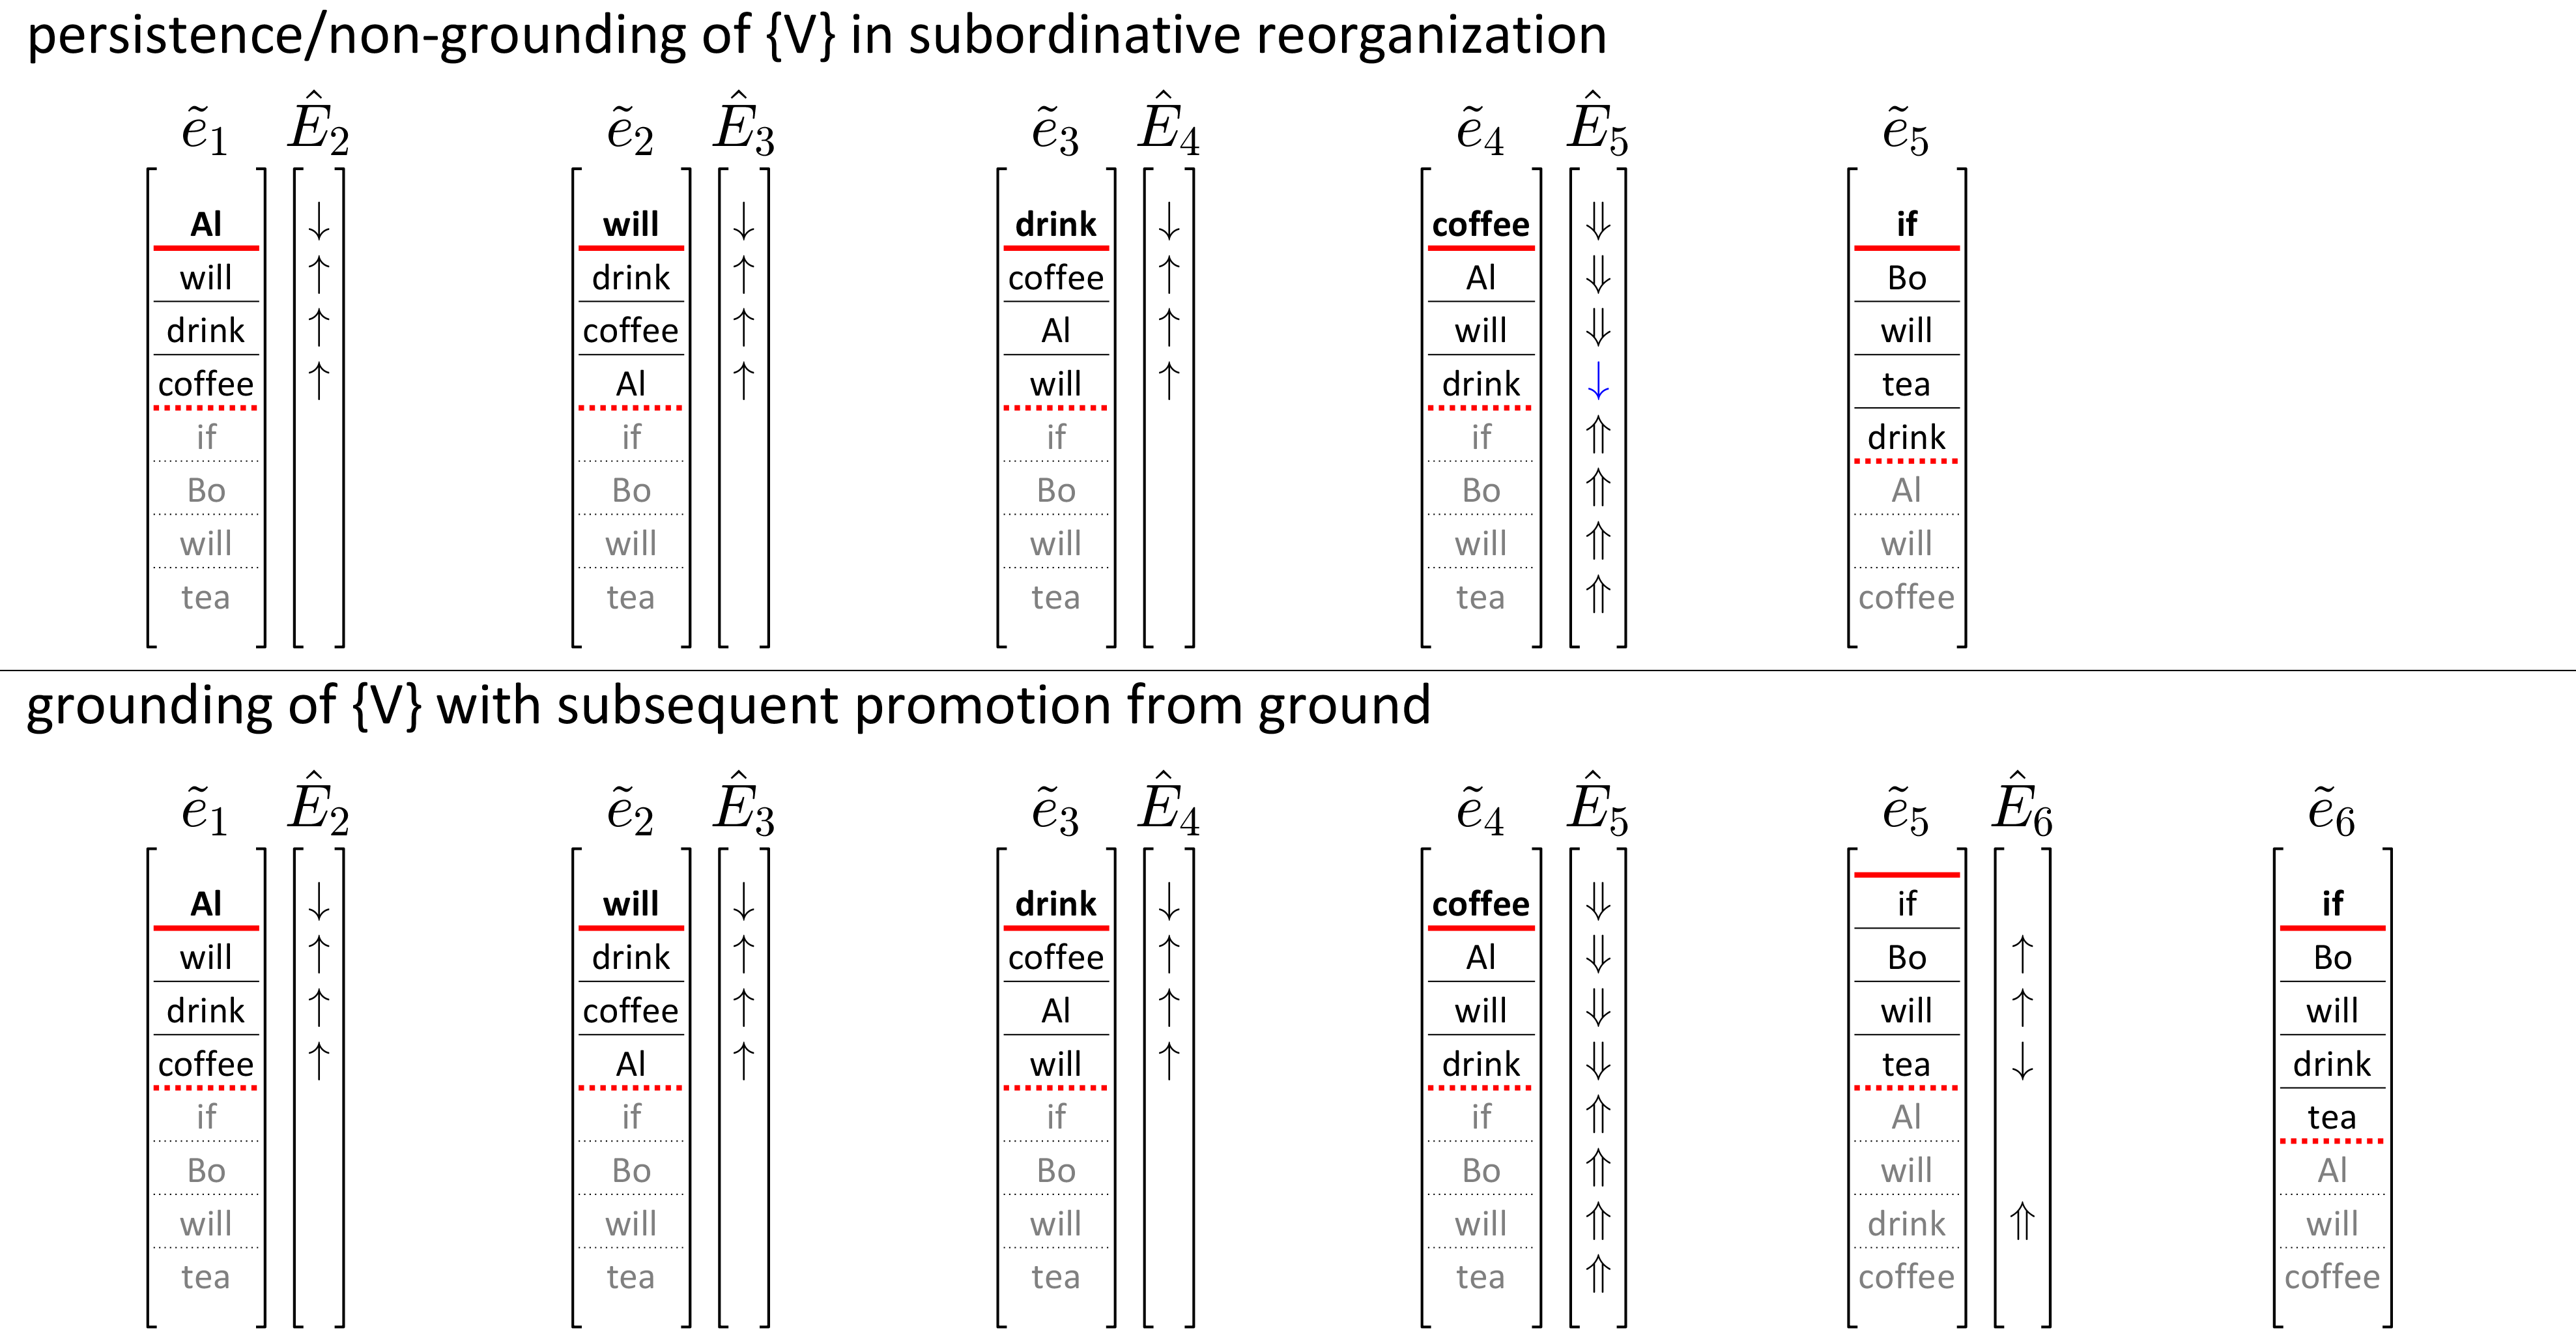
\includegraphics[width=\textwidth]{figures/Tilsen-img149.png}
\caption{\missingcaption}
\label{fig:7:5}
\end{figure}
 

  In the above analyses, we have constructed two [will]\{aux\} systems by presupposing parallel differentiations of the c-system [will] and the s-system \{\textsc{aux}\}. However, we did not represent parallel c-/s- differentiations for [drink]\{V\}. As mentioned above, the excitation persistence mechanism can be interpreted as a manifestation of parallel differentiation of [drink]\{V\}. In other words, we can imagine that that there are two [drink]\{V\} cs-systems which are highly overlapping and thus interact strongly. Ellipsis is often possible precisely when parallel c-/s- differentiation of a lexical system occurs in association with different clauses. Parallel c-/s- differentiation can thus be seen as a state which induces non-selection of excited systems. Subordinative reorganization can in this light be viewed to interfere with parallel c-/s- differentiation of lexical cs-systems, while assisted persistence—in the form of coupling with an \{\textsc{aux}\} system—can stabilize parallel c-/s- differentiation.

\subsection{Reiterative facilitation of persistent excitation}

The above analyses can be generalized to cases in which non-selection of a system precedes the selection of that same system. We accomplish this by applying the persistent excitation analysis to a reiterative trajectory. The interactions of this more general analysis with the varieties of ellipsis above (gapping, stripping, VP ellipsis, pseudogapping, etc.) are somewhat complicated and intuitions can be difficult to assess. For simplicity, we consider only the object NP ellipsis below (cf. \citealt{Wilder1997}). The ellipsis in a coordinated clause (a) seems to cohere more readily than examples (b) and (c), where one of the clauses is subordinate. The persistent excitation analysis developed above, with no further mechanism, predicts that none of the three trajectories should cohere because the non-selected cs-systems seem not to have been excited in any preceding epochs.

\ea
\ea[]{Al brews and Bo drinks coffee.}
\ex[?]{Al brews so Bo drinks coffee.}
\ex[?]{If Al brews, Bo drinks coffee.}
\z
\z

  However, recall that reiterative simulation creates periodic trajectories in which absolute notions of precedence become inapplicable. To account for the coherence of (a), we can imagine that the producer obtains a reiterative trajectory before selective production. In the trajectory below, (e0)-(e5) are reiterative and non-selective. The key insight is that when the trajectory transitions to a selective regime with reorganization Ê\textsubscript{6}, [coffee]\{N\} has already been excited and can remain so. Thus the presence of a reiteration prior to selective production allows for coherence of (e6) and (e7). What is more challenging to explain is the non-promotion of [coffee] in Ê\textsubscript{8}, which might be understood as an anticipatory reorganization of excitation for the second clause.

  
\begin{figure}
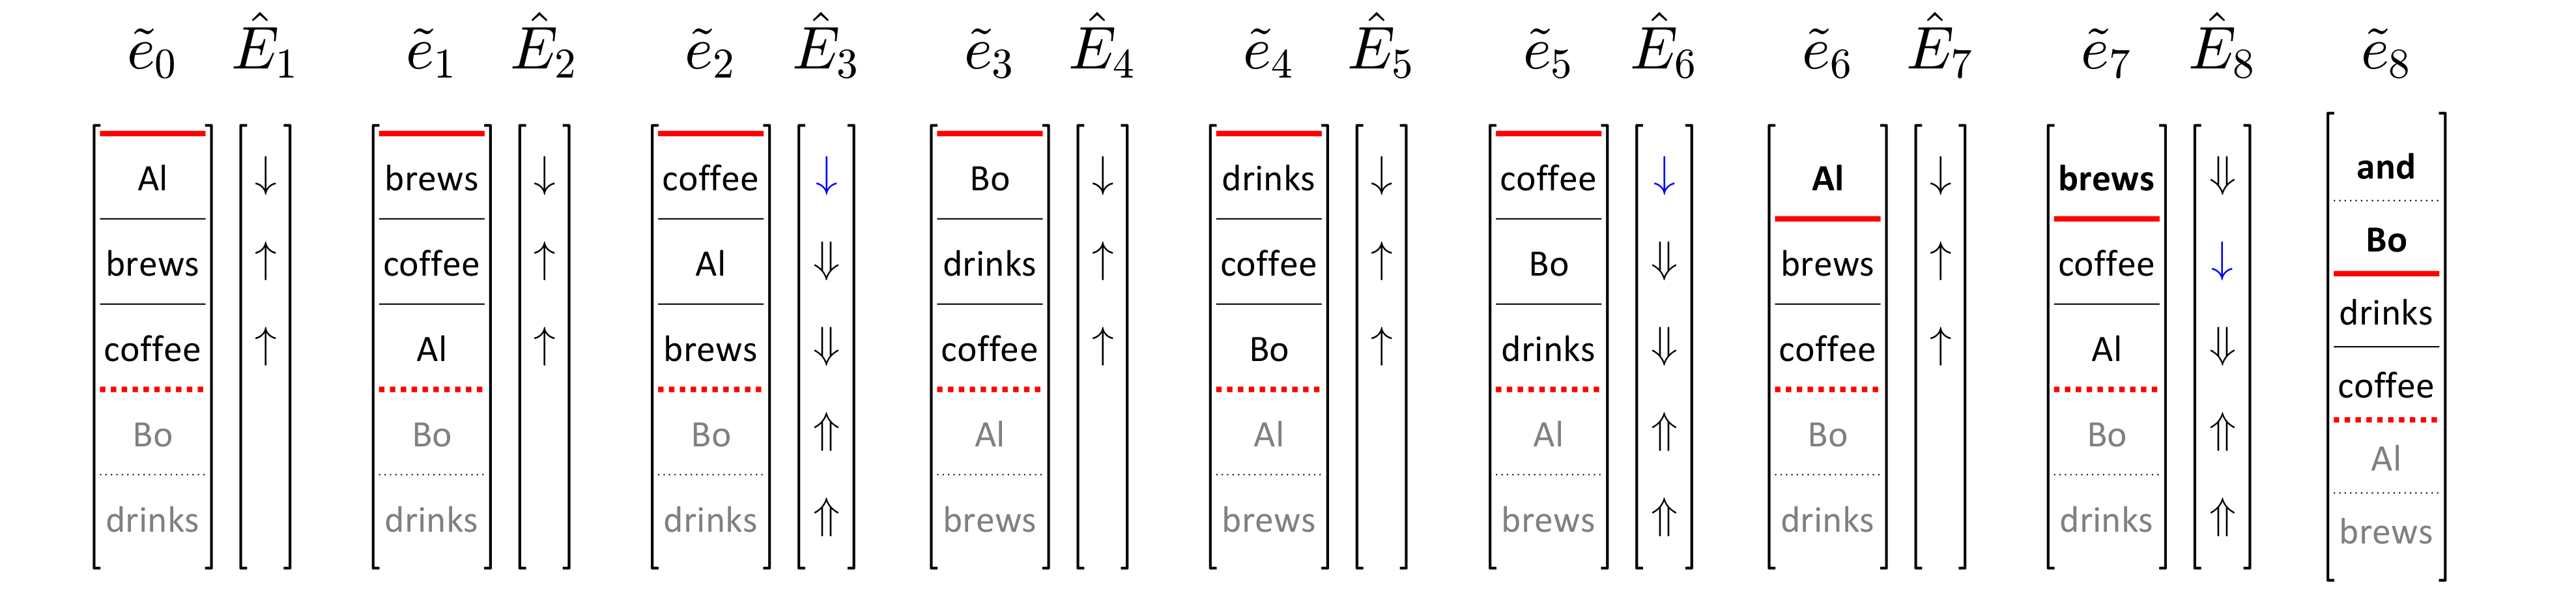
\includegraphics[width=\textwidth]{figures/Tilsen-img150.png}
\caption{\missingcaption}
\label{fig:7:6}
\end{figure}
 

  Why do the sentences with a subordinated clause in (b) and (c) fail to cohere as readily as the coordinated clauses in (a)? Presumably the distinction between coordinative and subordinative reorganization applies to reiterative trajectories as well. To account for non-coherence of example (c), we suspect that the subordinative reorganization destabilizes coupling of [brews]\{V\} with [coffee]\{N\} because it grounds [coffee]\{N\} in the reiterative trajectory. To account for non-coherence of (b), we could infer that initial organization, or organization of a main clause, also involves grounding demotions. Hence [coffee]\{N\} is not excited in epochs when [Al]\{N\} and [brews]\{V\} are excited, resulting in non-coherence. 

  The generalizations that emerge from the above analyses are as follows: only coordinative reorganizations allow unassisted persistence of excitation; subordinative and main-clause reorganizations ground previously excited systems; some other mechanism, such as assisted persistence, is required to maintain excitation of systems through a subordinative or main-clause reorganization. 

\subsection{Contextual excitation and ellipsis}

Another influence on coherence of ellipsis is excitation of systems by discourse context. Contextually excited cs-systems which, despite not being selected in the same sentence, and perhaps never being selected at all, can participate in φ configurations if they have above-ground excitation. Consider answer ellipsis examples below.

\ea
   \ea    S1: \textit{Who drank coffee?}  S2: \textit{Al}.
    \ex    S1: \textit{What did Al drink?}   S2: \textit{Coffee.}
\z
\z

  In these examples, cs-systems which were excited for S2 as an interpreter of S1 may not be promoted to selection level for S2 as a producer. Hence for the question response in (a), [drank]\{V\} and [coffee]\{N\} are excited in a production trajectory for S2, but may not be selected. These systems can nonetheless can participate in the {\textbar}Al drank coffee{\textbar} φ configuration. As shown below, S2 will couple the selected cs-system of the response to the relevant wh-system, which remains active in production epochs (e1)-(e3). In a sense, our analysis has the spirit of analyses in which answer fragments have “fully sentential structures”  \citep{Merchant2005}, but our conceptualization of structure here is radically different.

  
\begin{figure}
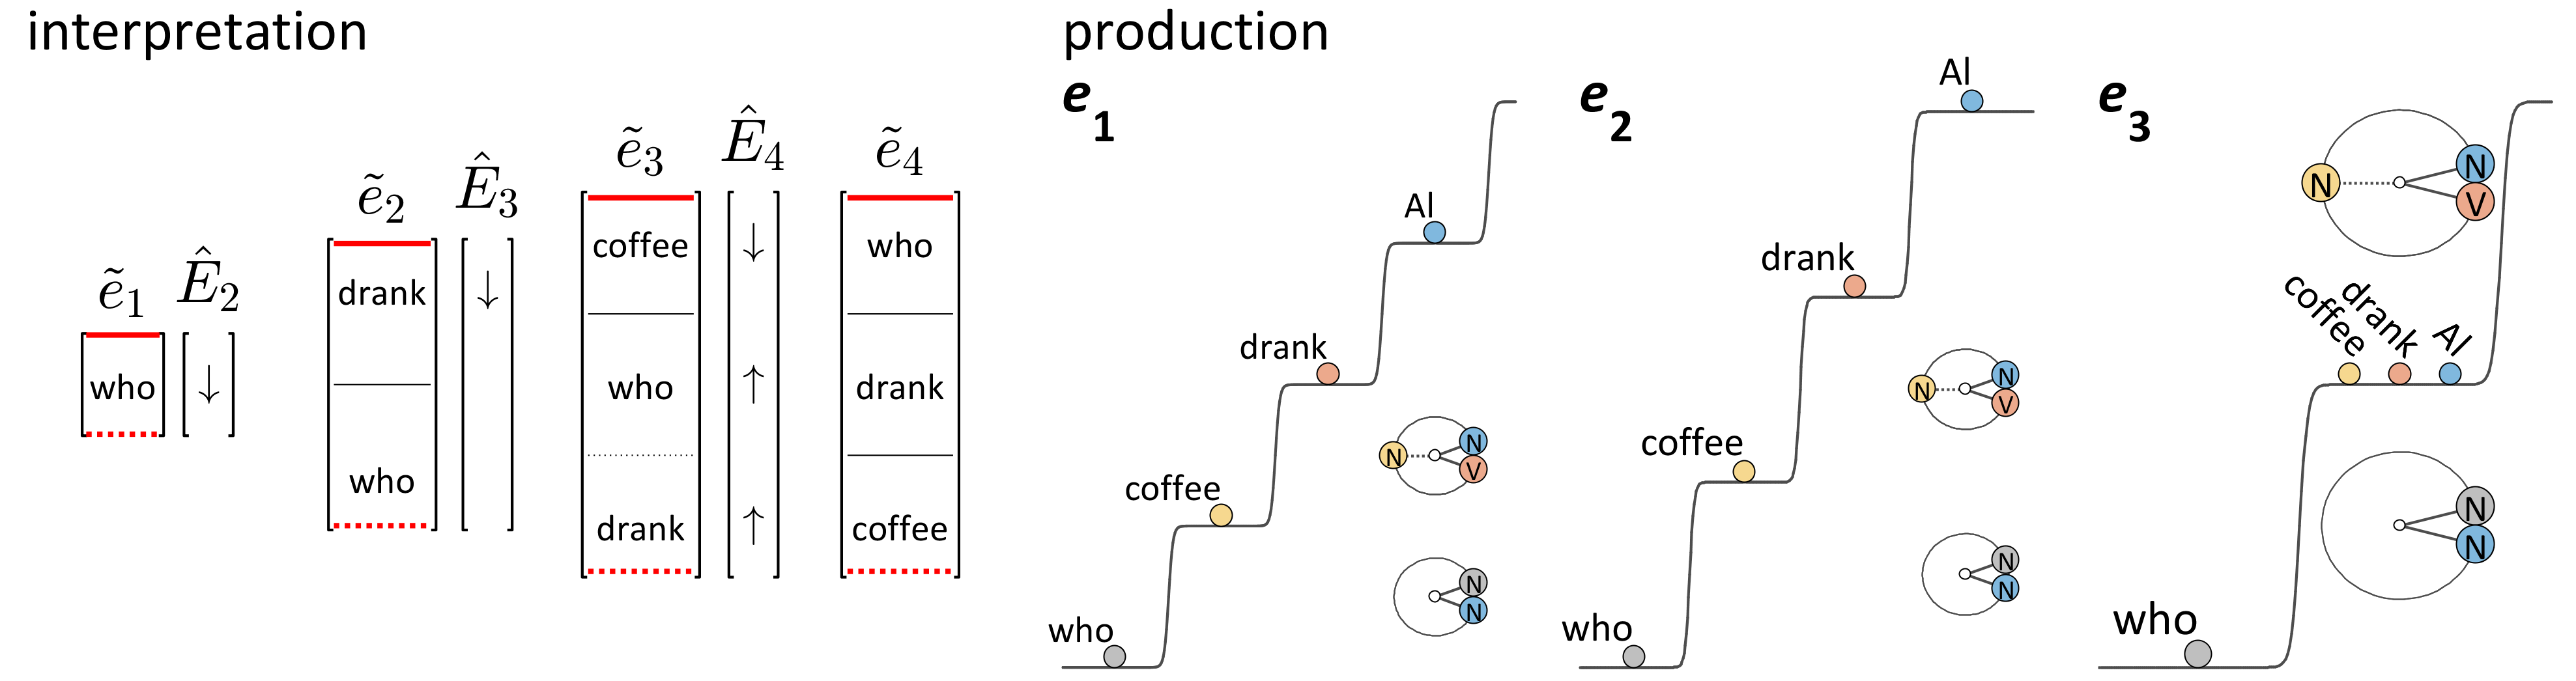
\includegraphics[width=\textwidth]{figures/Tilsen-img151.png}
\caption{\missingcaption}
\label{fig:7:7}
\end{figure}
 

  In the above analyses, we have established a viable set of analytic tools for understanding various aspects of the phenomenon of ellipsis. These tools include persistent excitation, assistance of persistent excitation through coupling to excited systems, and reiterative trajectories which precede selective production. In combination with hypothesized differences in grounding propensities of coordinative vs. subordinative/main clause reorganizations, the analytic tools can explain a variety of ellipsis patterns. Further evidence of their utility comes from applying them to other phenomena, such as anaphora.

\section{Anaphora}

From the conventional perspective, anaphora is occurrence of an expression (syntactic object) whose interpretation depends on the presence of another object, and coreference is the more general circumstance in which two expressions refer to the same person or thing (\citealt{HankamerSag1976,Huang2000,Reinhart1983,Reinhart2016,Safir2004}). In the example below, anaphors and their coreferent expressions are indexed:

\ea
    {Al\textsubscript{i} brews coffee\textsubscript{j} and he\textsubscript{i} drinks it\textsubscript{j}}.
\z

  There are a number of sensible questions from this perspective, such as whether there are structural constraints on coreference patterns and on the temporal ordering of coreferent expressions in sentences. From an o/el perspective, we reframe these questions, asking what conditions induce the selection of anaphors in production trajectories. The focus here is on nominal anaphora, with the presumption the account can be extended to verbal anaphora. 

\subsection{Anaphoric systems}

Because of their unique behavior, we posit a new class of s-system for anaphors: \{\textsc{pro}\}, and also a class of anaphoric c-systems, which we label generically as [\textsc{pro}]. As expected, these systems form cs-resonances,  \{\textsc{pro}\} differentiates readily into \{+\textsc{pro}\} and \{-\textsc{pro}\}, and \{\textsc{pro}\} can be co-selected with a variety of grammatical s-systems, e.g. \{\textsc{person}\}, \{\textsc{number}\}, \{\textsc{gender}\}. The \{\textsc{pro}\} s-system is unlike \{N\} in that \{ADJ\} and \{D\} systems do not readily φ couple with \{\textsc{pro}\} (i.e. *\textit{the cold it}). The [\textsc{pro}] c-system is unusual in that it evokes a nonspecific meaning, and we hypothesize that in typical uses, the specificity of meaning experiences from φ configurations with \{\textsc{pro}\} results from +φ coupling between \{\textsc{pro}\} and some other excited system. This system may be excited from contextual forces, may have been excited earlier in an utterance, or may be excited in a reiterative trajectory preceding selective production. 

   Consider the utterance \textit{he drinks it} and two possible initial configurations of production, shown below. The state in (A), in which no lexical \{N\} systems are excited, cannot give rise to a coherent meaning experience. Instead we hypothesize an initial configuration such as (B), where each \{\textsc{pro}\} is coupled to an excited lexical s-system. These lexical systems are not promoted to selection during production. Another somewhat atypical characteristic of [\textsc{pro}]\{\textsc{pro}\} systems is that their gm-domains tend to vary as a function of co-selected grammatical systems. The set of co-selected grammatical s-systems determines the gm-domain of [\textsc{pro}]\{\textsc{pro}\}, as represented in (B). For clarity, we usually omit these grammatical systems from representations.   

  
\begin{figure}
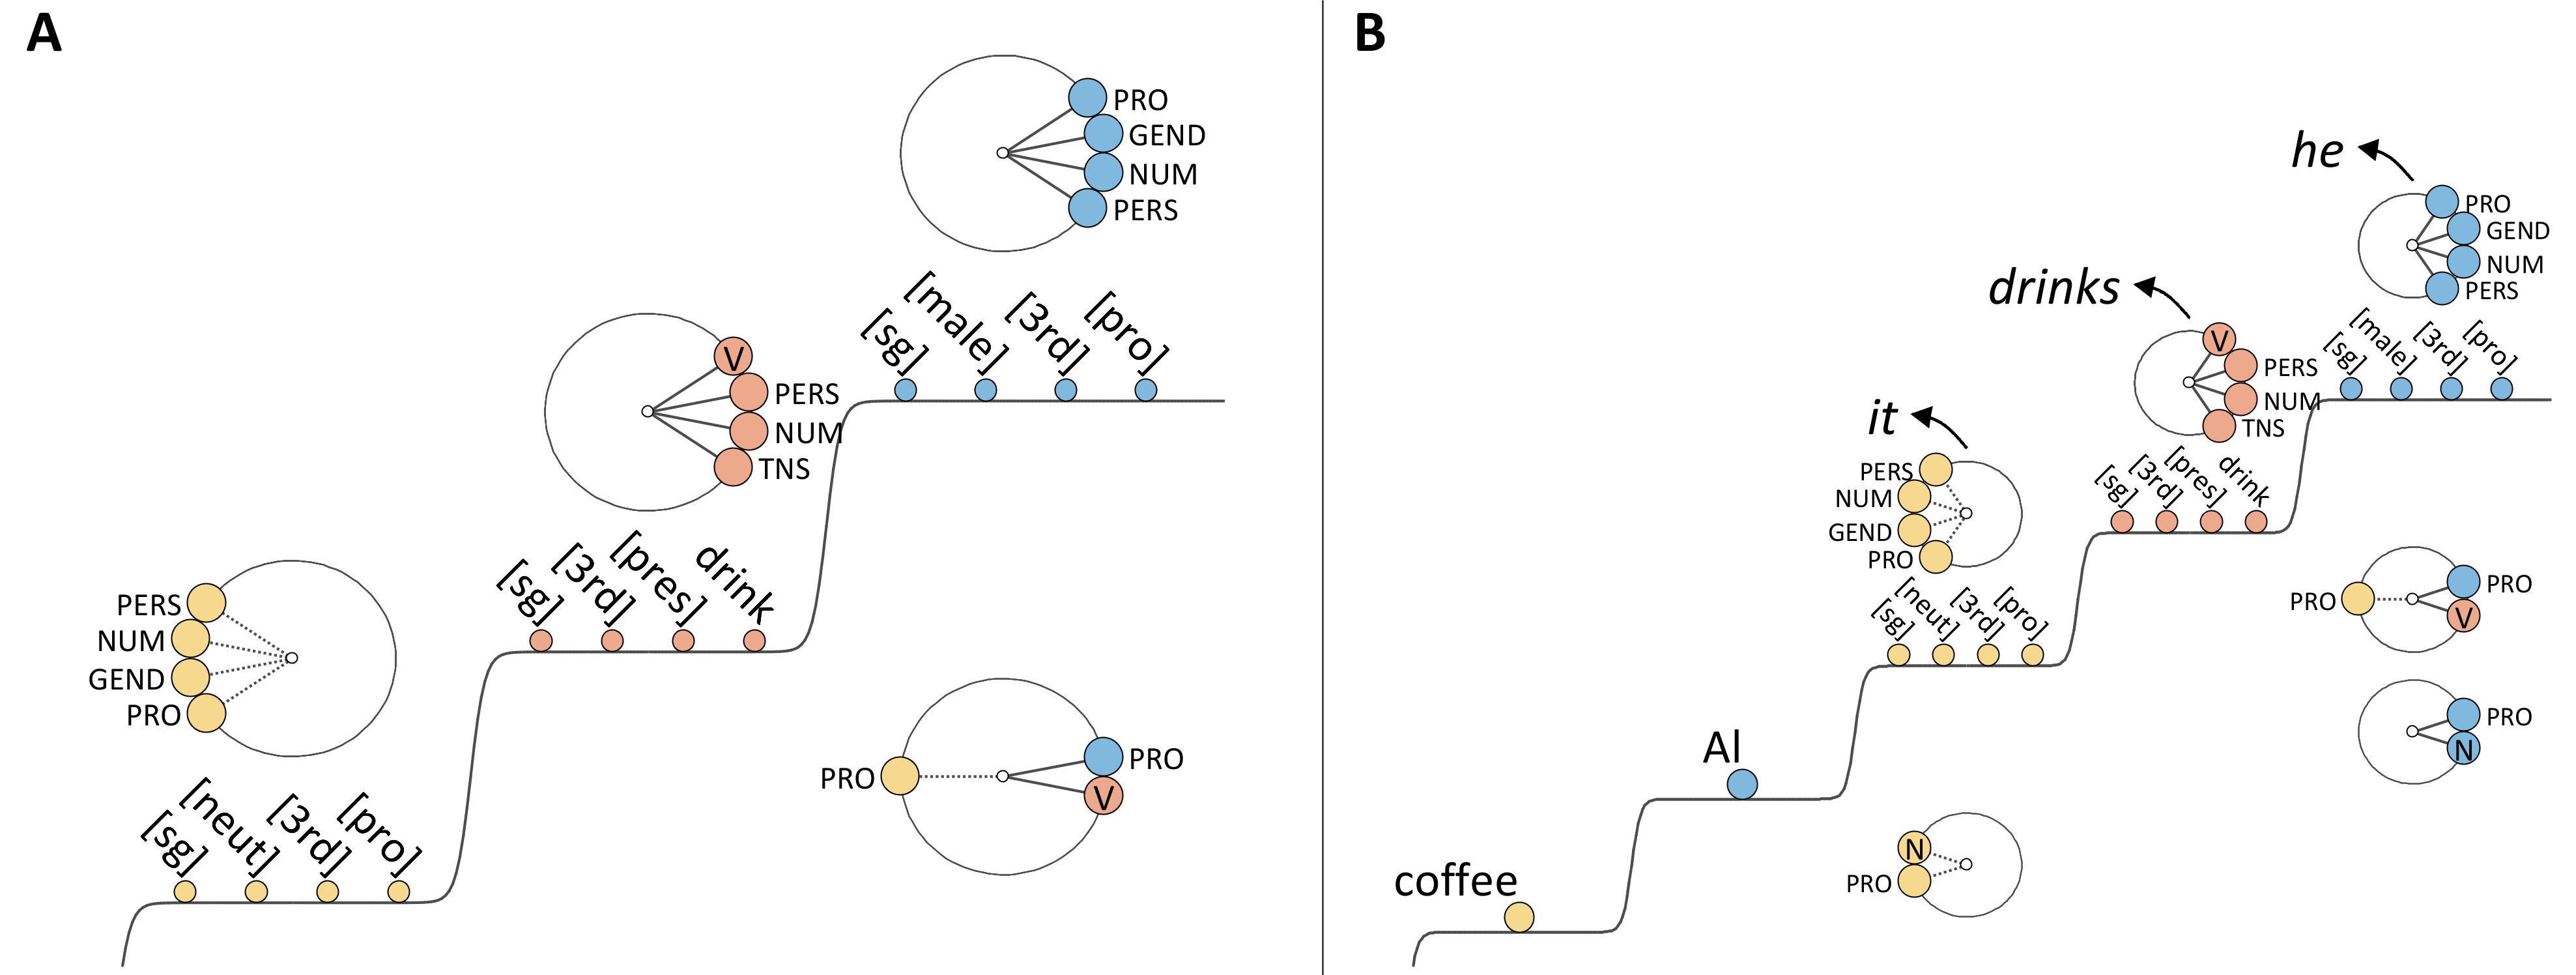
\includegraphics[width=\textwidth]{figures/Tilsen-img152.png}
\caption{\missingcaption}
\label{fig:7:8}
\end{figure}
 

  The excitation of a \{\textsc{pro}\} system is an alternative and less direct mechanism for stabilizing a φ configuration. For coherence to occur, each \{\textsc{pro}\} must be coupled to a lexical cs-system. An even stronger account posits that excitation of an \{N\} system always activates a corresponding \{\textsc{pro}\} system. For example, in the utterance below we could imagine that during epochs in which the first clause is attended (e.g. e1), \{\textsc{pro}\} systems coupled to \{N\}[Al] and \{N\}[coffee] are activated. In later epochs (e.g. e2) with attention on the second clause, those \{PRO\} systems are excited and are promoted to selection instead of [Al]\{N\} and [coffee]\{N\}. The lexical systems nonetheless remain above ground, another example of persistent excitation. Moreover, because coherence occurs with anaphors in a subordinated clause (e.g. \textit{Al drinks coffee, if he brews it}), we infer that \{\textsc{pro}\} systems facilitate the persistence of excitation of the lexical system with which they are coupled. Thus the excitation of \{\textsc{pro}\} systems by Ê\textsubscript{4} keeps [Al]\{N\} and [coffee]\{N\} above ground.

  \ea
  {Al drinks coffee, and he brews it.}
\z
  
\begin{figure}
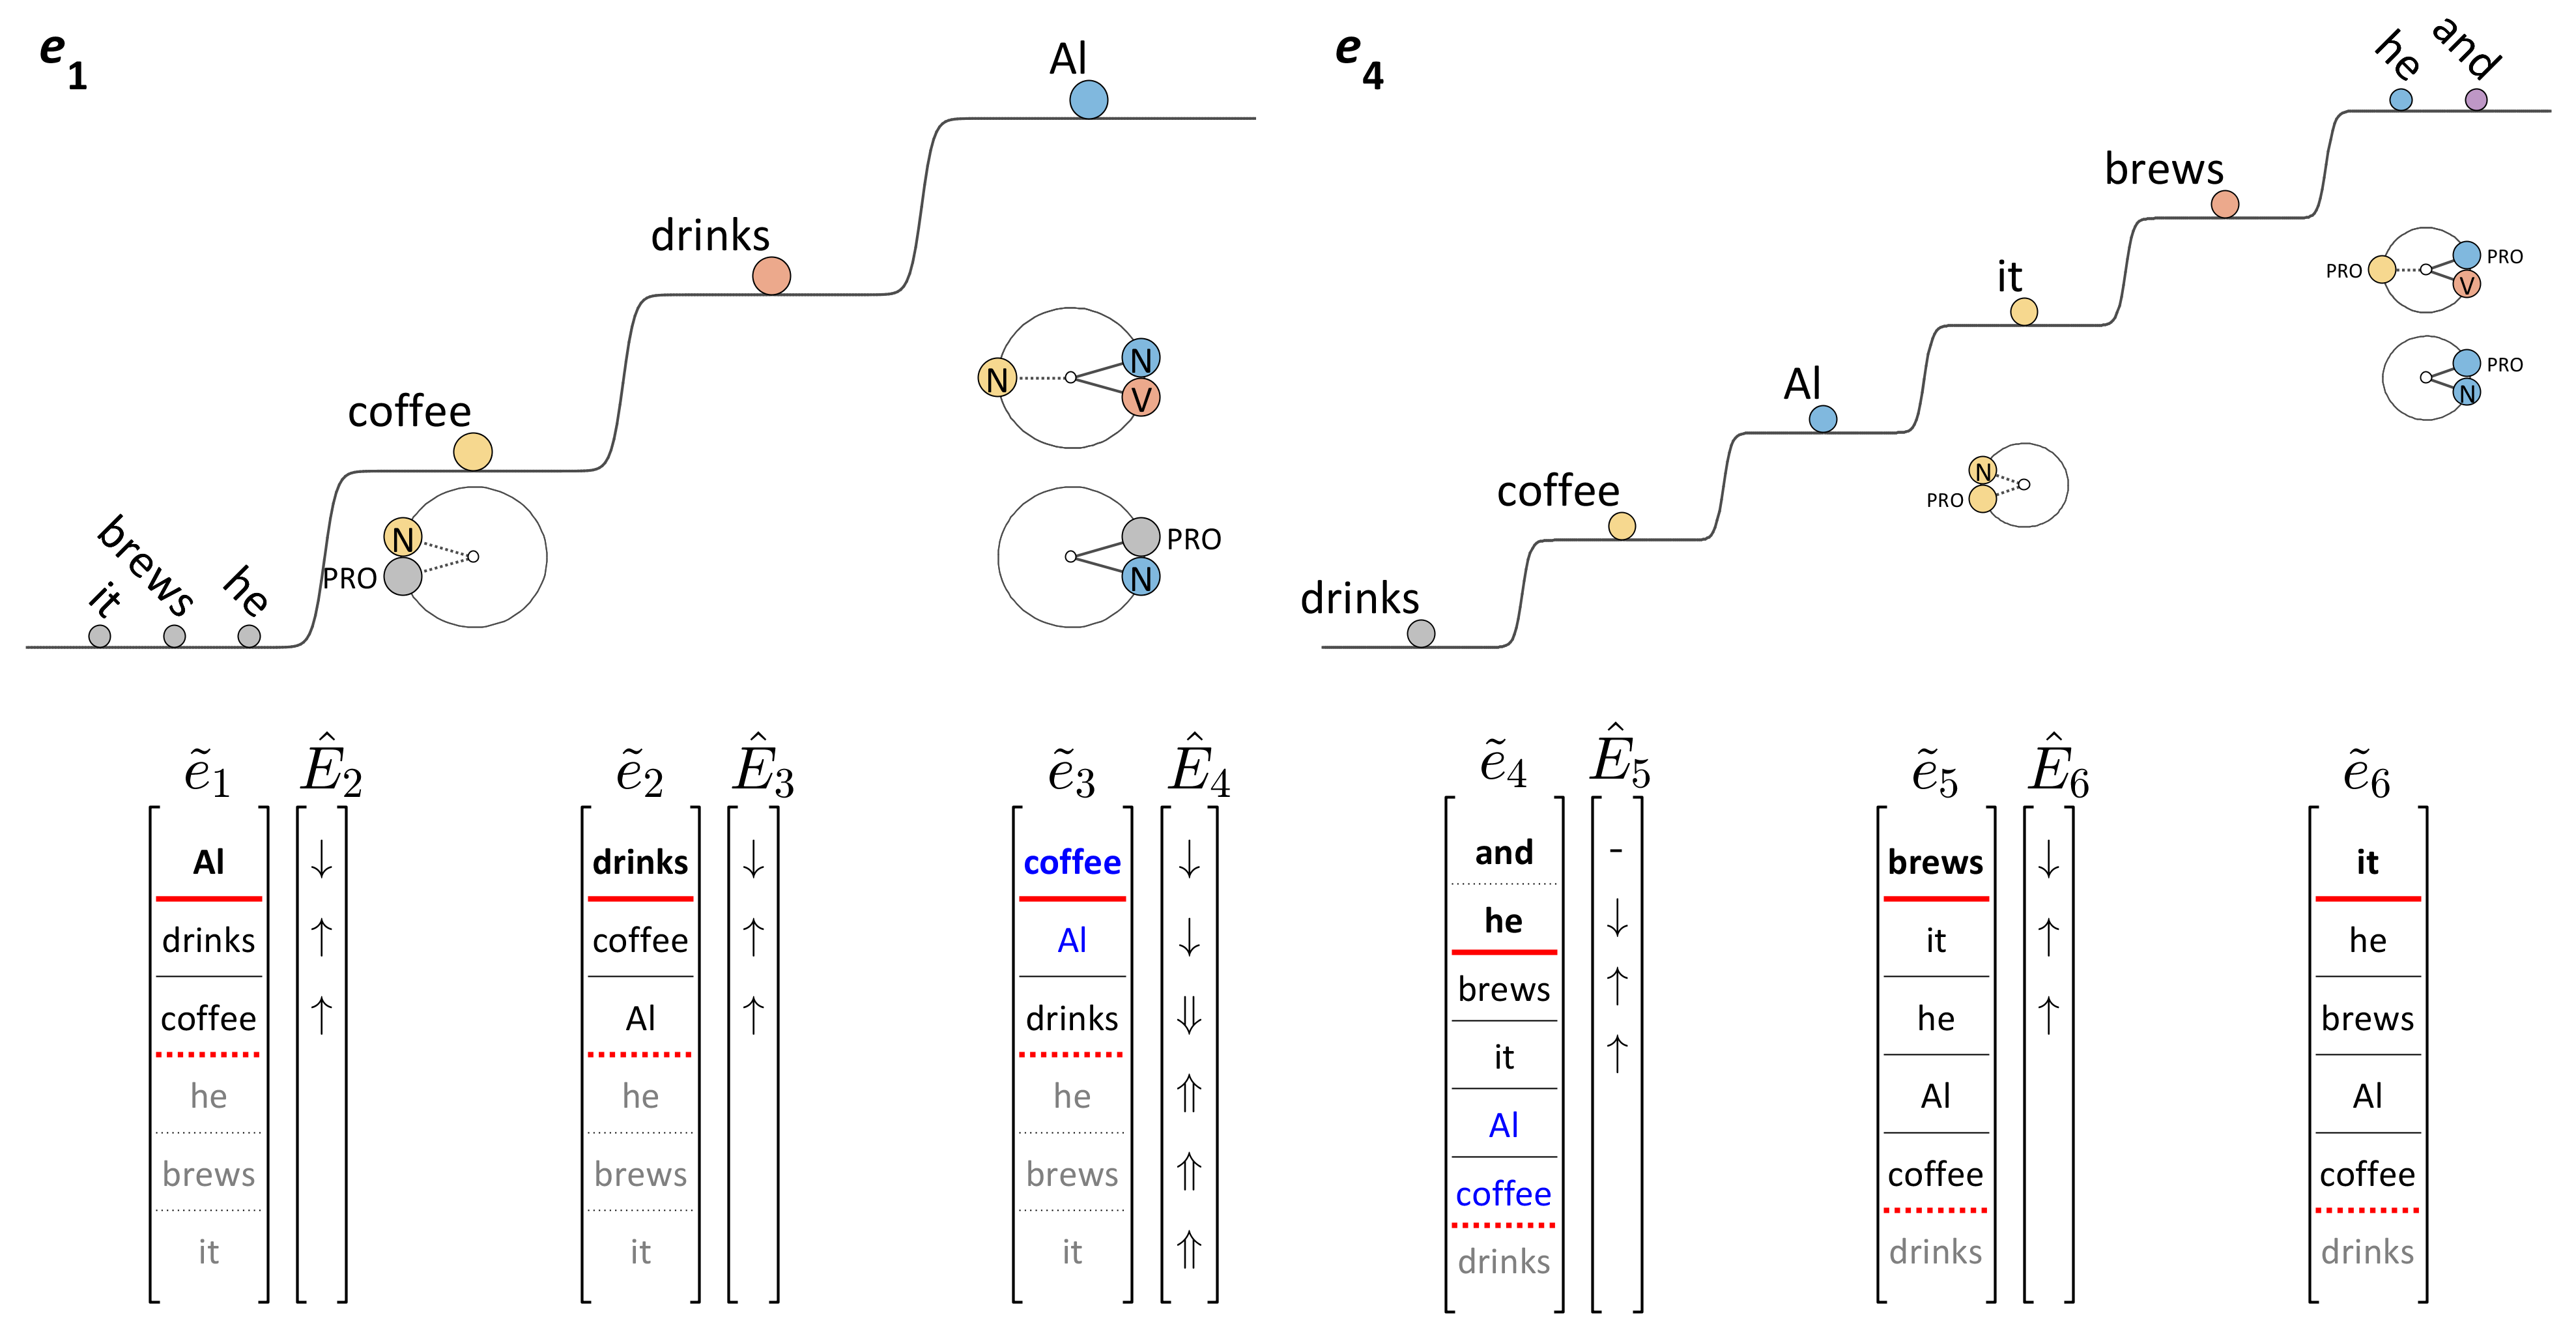
\includegraphics[width=\textwidth]{figures/Tilsen-img153.png}
\caption{\missingcaption}
\label{fig:7:9}
\end{figure}
 

  One of the interesting characteristics of \{\textsc{pro}\} systems is that there is evidently a bias to select them instead of lexical systems, but only when the relevant lexical system has already been selected. The bias is not an obligation, since productions can occur such as \textit{Al drinks coffee, and Al brews coffee}. Nonetheless, an explanation for the \{\textsc{pro}\} bias is desirable. One possible mechanism to create a bias for promotion of \{PRO\} rather than \{N\} may involve recent demotion of the conceptual and/or gestural systems associated with lexical cs-system. In other words, recently demoted systems may be less amenable to be subsequently promoted.

  Anaphora is similar to ellipsis, in that it occurs when parallel c-system and s-system differentiation might be required. Generally, we can view anaphora and ellipsis, along with direct reference, as three different classes of trajectories for evoking a meaning experience. Some examples of these are compared in the {\tablebelow}. 

  \begin{table}
\begin{tabularx}{\textwidth}{QQQQ}
\lsptoprule
& cs-system & cs-system

selected & φ configurations

of second clause\\
\midrule 
\textbf{Direct reference}

\textit{Al drinks} tea \textit{and \textit{Al} drinks coffee} & [Al]\{N\} & yes & {\textbar}Al drinks coffee{\textbar} \\

\tablevspace
\textbf{Anaphora}\\
\midrule 

\textit{Al drinks tea, and \textit{he} drinks coffee} & [\textsc{pro}]\{\textsc{pro}\} & yes & {\textbar}\textsc{pro} drinks coffee{\textbar} 

{\textbar}\textsc{pro} Al{\textbar} \\

\tablevspace
\textbf{Ellipsis}\\
\midrule 

\textit{Al drinks tea, and \textsubscript{(Al)} drinks coffee} & [Al]\{N\} & no & {\textbar}Al drinks coffee{\textbar} \\

\tablevspace
\textbf{Null pronominal}\\
\midrule 

\textit{Al wants to} (\textsc{pro}) \textit{drink coffee} & [\textsc{pro}]\{\textsc{pro}\} & no & {\textbar}\textsc{pro} drinks coffee{\textbar} 

{\textbar}\textsc{pro} Al{\textbar} \\
\lspbottomrule
\end{tabularx}
\caption{\missingcaption}\label{tab:7:2}
\end{table}

Direct reference and ellipsis create relational meaning experiences from φ configurations directly through coupling of lexical s-systems. In contrast, anaphora creates relational meaning more indirectly. For example, by coupling to both [Al]\{N\} and [drinks]\{V\}, \{\textsc{pro}\} indirectly brings about the φ configuration {\textbar}Al drinks coffee{\textbar}. In direct reference and anaphora, the relevant cs-system which participates in the φ configuration(s) is selected; in ellipsis, this cs-system is not selected. Given this taxonomy of reference, a logical possibility is a non-selected [\textsc{pro}]\{\textsc{pro}\} system giving rise to a φ configuration indirectly. This could correspond to a null pronominal or big \textsc{pro}, as in \textit{Al wants pro to drink coffee}.

\subsection{Temporal ordering of anaphoric and lexical systems}

In some circumstances, an anaphor and its lexical antecedent can be selected in either temporal order, as shown by the example of backward anaphora in \REF{ex:7:1b} below (cf. \citealt{KazaninaEtAl2007,ReulandAvrutin2005}). In conventional approaches, such examples violate a hypothesized principle requiring antecedents to “precede” anaphors in a structural sense, and hence necessitate a movement analysis \citep{Chomsky1993}. Instead of moving object structures, we can understand such phenomena to be associated with a reiterative trajectory, just as we did for ellipses.

  We imagine that the reiterative trajectory in (e0)-(e6) precedes selective production of the utterance. Thus the lexical antecedent of the matrix clause can persist in an excited state when overt production of the subordinate clause occurs. The utterances \REF{ex:7:1a} and \REF{ex:7:1b} can be distinguished according to when, in the context of the reiteration, production transitions to a selective regime. When the transition occurs in conjunction with a reorganization to (e0), sentence \REF{ex:7:1a} is produced; when the transition occurs with reorganization to (e3), sentence \REF{ex:7:1b} is produced. In this case, promotion of [it]\{\textsc{pro}\} assists the persistence of [coffee]\{N\}, which was excited in the preceding epochs of the reiteration.

\ea\label{ex:7:1}
\ea{\label{ex:7:1a}Al drinks coffee, when Bo brews it.}
\ex{\label{ex:7:1b}When Bo brews it, Al drinks coffee.}    
\z
\z
  
\begin{figure}
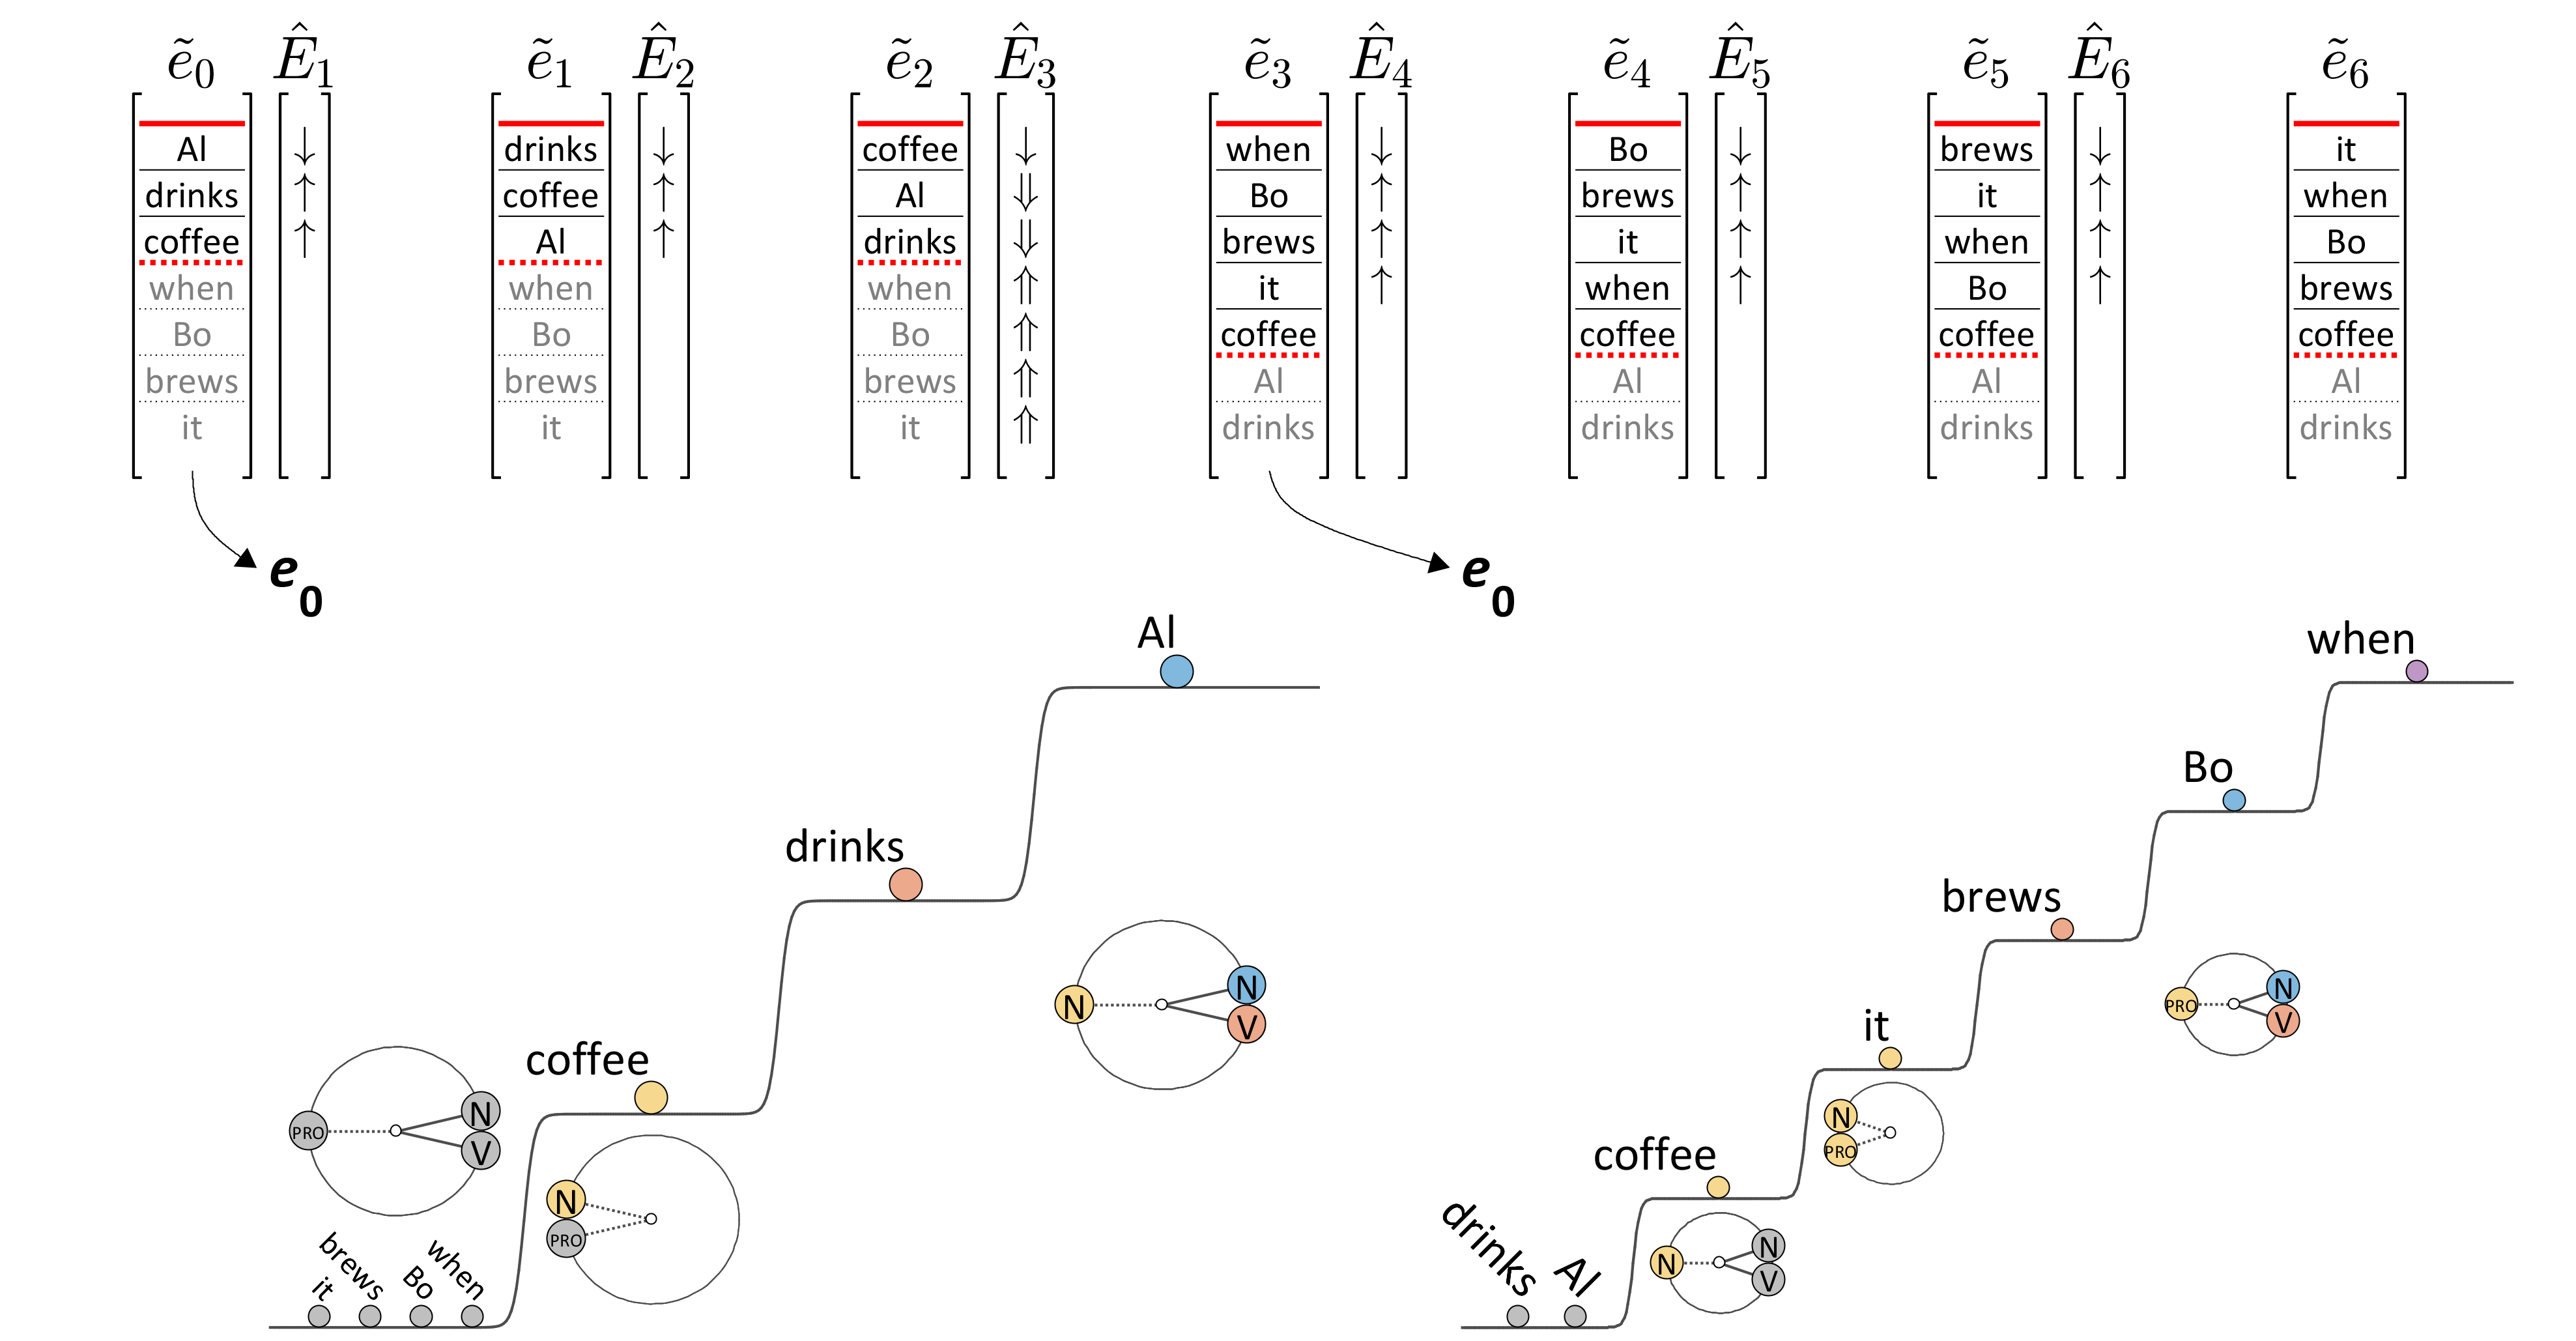
\includegraphics[width=\textwidth]{figures/Tilsen-img154.png}
\caption{\missingcaption}
\label{fig:7:10}
\end{figure}
 

  However, the coherence contrast between the examples in \REF{ex:7:2} below suggests that reorganization to a main clause exerts a stronger grounding force on systems than reorganization to a subordinate or coordinated clause. When a production trajectory transitions to a selective regime and a main clause, all systems are grounded, except those associated with the main clause. Hence [coffee]\{N\} is grounded during attention to the relevant φ configuration in \REF{ex:7:2b}, rendering the trajectory noncoherent. In the trajectory for \REF{ex:7:2b} below, we show a reiteration of epochs (e0)-(e6). Note that the reorganization of attention to the main clause (Ê\textsubscript{7}) demotes [coffee]\{N\} to ground, and hence [coffee]\{N\} is not available when production subsequently transitions to a selective regime. Of course, with some effort, [coffee]\{N\} can be promoted to an excited state in this transition, and we suspect that this accounts for variation in coherence intuitions. 

\ea\label{ex:7:2}
  \ea[]{\label{ex:7:2a}Al drinks coffee, and/when Bo brews it.}  
   \ex[?]{\label{ex:7:2b}Al drinks it, and/when Bo brews coffee.}
\z
\z
  
\begin{figure}
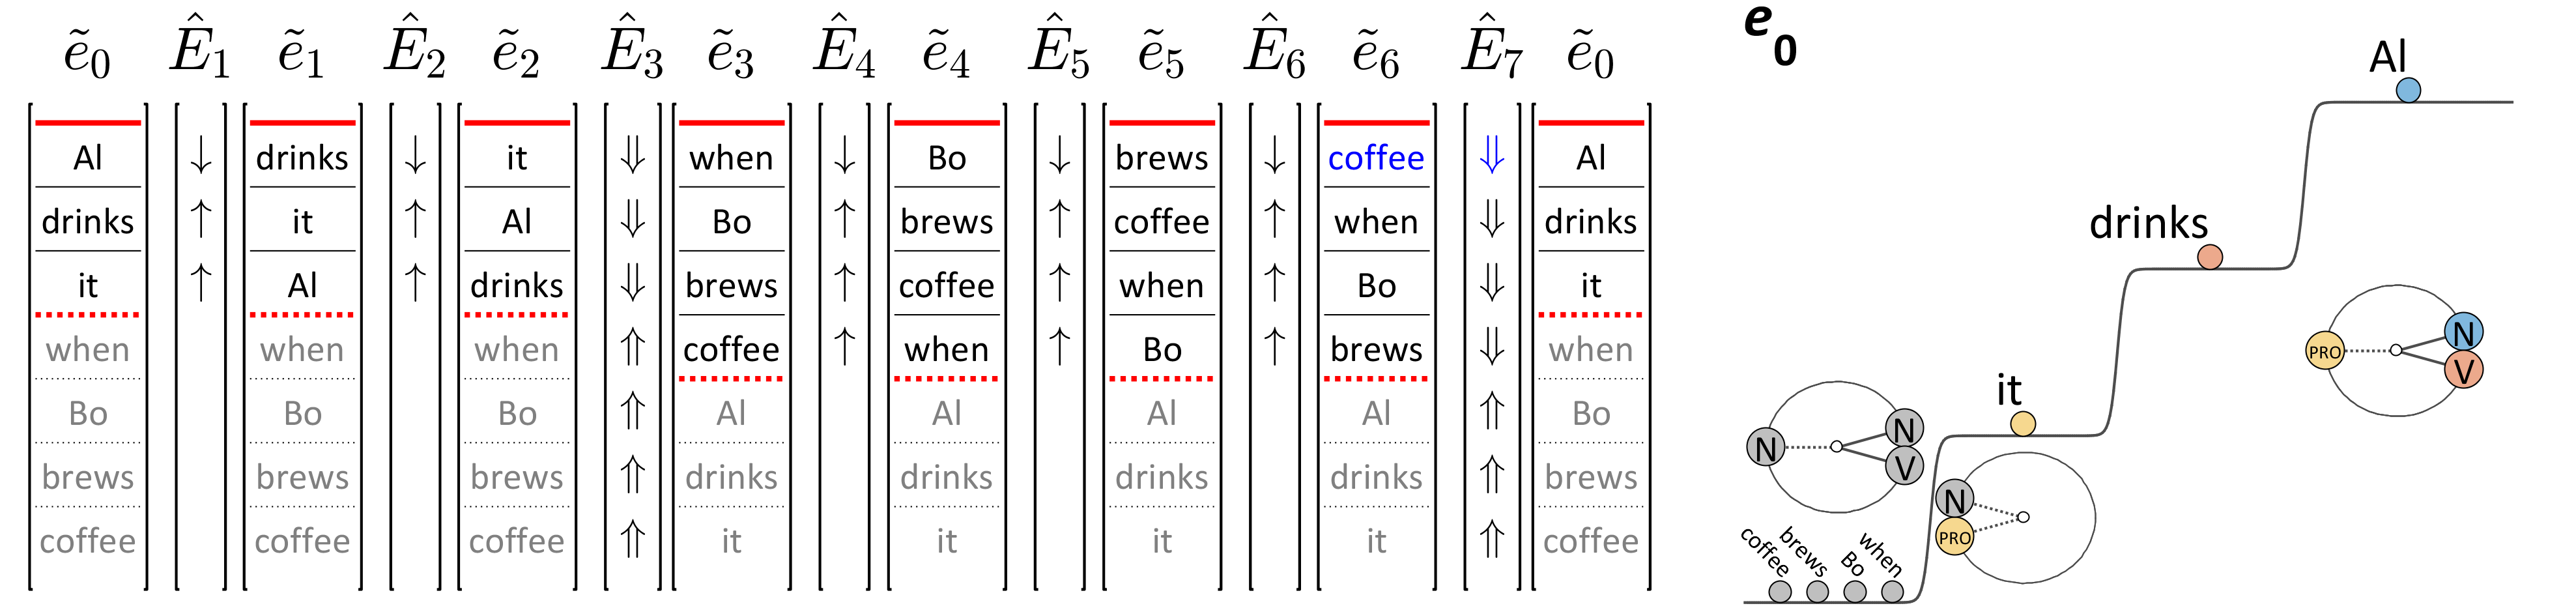
\includegraphics[width=\textwidth]{figures/Tilsen-img155.png}
\caption{\missingcaption}
\label{fig:7:11}
\end{figure}
 

  From the perspective of interpretation, sentence \REF{ex:7:2b} may evoke an exophoric relation between [it]\{PRO\} and a contextually activated system. Because of the immediate organization bias, an interpretation trajectory may involve excitation of a lexical \{N\} system which is not selected in an utterance, and this would naturally interfere with the intended interpretation. 

  The analyses we have developed of anaphora and ellipsis are based on the idea that various characteristics of a reorganization influence the propensity for a lexical cs-system to remain excited. For ellipsis we observed that persistence of an elided cs-system is assisted when the system is coupled to another above-ground system, such an \{\textsc{aux}\} system. For anaphora, we interpret \{\textsc{pro}\} as an assisting system of this sort. In both cases, when a reiterative regime precedes a selective one, the normal temporal relation of antecedent/dependent relations can be reversed. Moreover, the analyses indicate a hierarchy of reorganizations based on the propensity of the reorganization to ground a system that has a promoted competitor:

\begin{table}
\begin{tabularx}{\textwidth}{Xl}
\lsptoprule
non-grounding & canonical reorganization within clause\\
& selective reorg. to coordinated clause\\
& selective reorg. to coordinated system within-clause\\
weakly grounding & selective reorg. to subordinate clause\\
strongly grounding & selective reorg. to main clause\\
\lspbottomrule
\end{tabularx}
\caption{\missingcaption}\label{tab:7:3}
\end{table}

  This reorganization-grounding hierarchy is a key aspect of our analyses of ellipsis and anaphora patterns. It is important to recognize that such analyses are only necessary because we have rejected the assumption that systems associated with different clauses are equivalently co-present. This rejection is desirable because of differentiation interference, which derives from the microscale model of differentiation. Moreover, we show below that differentiation motivates a novel analysis of binding.

\subsection{Binding theory}

In general the forces which influence whether an anaphoric \{\textsc{pro}\} or lexical system is promoted to selection level are not so strong that only one option is possible. Both anaphoric and direct reference options are available in many contexts, although re-selection of the lexical cs-system tends to sound somewhat overly formal:

\ea
   \ea{Al likes coffee and Bo likes coffee.}
    \ex{Al likes coffee and Bo likes it.}
\z
\z

  The biasing forces for selection of \{\textsc{pro}\} over a lexical system are stronger when the coreference obtains between two systems that participate in a φ configuration with the same lexical system, as in the examples below. The conventional approach to this phenomenon is to identify a structural pattern (“binding domain”) in which coreference obligates the reflexive form (\citealt{Chomsky1982,Chomsky1993,Haegeman1994,Reinhart1976,Safir2004}). From an o/el perspective, no such structure exists and therefore an alternative analysis is needed. To that end, we observe that reflexives are strongly preferred in a fairly unique configuration, one in which a c-system and an s-system differentiate in parallel and the differentiated systems obtain -φ relations. Following the earlier analysis of pronoun gm-domains, we begin by assuming that reflexive forms (i.e. \textit{myself}, \textit{ourselves}, \textit{yourself}…) are the gm-domain of a [\textsc{self}]\{\textsc{pro}\} cs-system, i.e. that there is a [\textsc{self}] c-system which is a subclass of [\textsc{pro}], and that the gm-domain of [\textsc{self}] is determined by co-selected grammatical s-systems for [\textsc{person}], [\textsc{number}], [\textsc{gender}], etc. 

\ea
\ea[]{Al\textsubscript{i} likes himself\textsubscript{i}}.      
\ex[*]{Al\textsubscript{i} likes him\textsubscript{i}}.        
\z
\z

  To motivate an o/el analysis of reflexives, we observe that there is a unique pattern of interference in the prototypical reflexive construction, in which a \{V\} is coupled to both a \{+N\} agent and a \{-N\} patient, and both of these \{N\} are coupled to the same c-system. We show this circumstance in (A) below, where the following conditions are required: \{\textsc{pro}\} must be +φ coupled to an excited lexical system, here [Al]\{-N\}; \{\textsc{pro}\} must be -φ coupled to [likes]\{V\}; and [Al]\{+N\} must be +φ coupled with [likes]\{V\}. It follows from transitivity of coupling that the only way for such a configuration to be stable is for [Al] to differentiate such that there is a [Al]\{+N\} system and a [Al]\{-N\} system. In other words, the differentiated [Al] systems have a distal φ relation; we call this a \textit{destructive c-differentiation}. States of destructive c-differentiation in particular are associated with strong preference for the reflexive form. The trajectory in (B) shows that the destructive c-differentiation must apply to c-systems which are excited in the same epoch, i.e. simultaneously attended, in order to induce excitation of the [\textsc{self}] system. 

\ea
\ea{Al\textsubscript{i} likes himself\textsubscript{i}}.  
\ex{Al\textsubscript{i} likes Bo, and Bo likes him\textsubscript{i}}.  
\z
\z
  
\begin{figure}
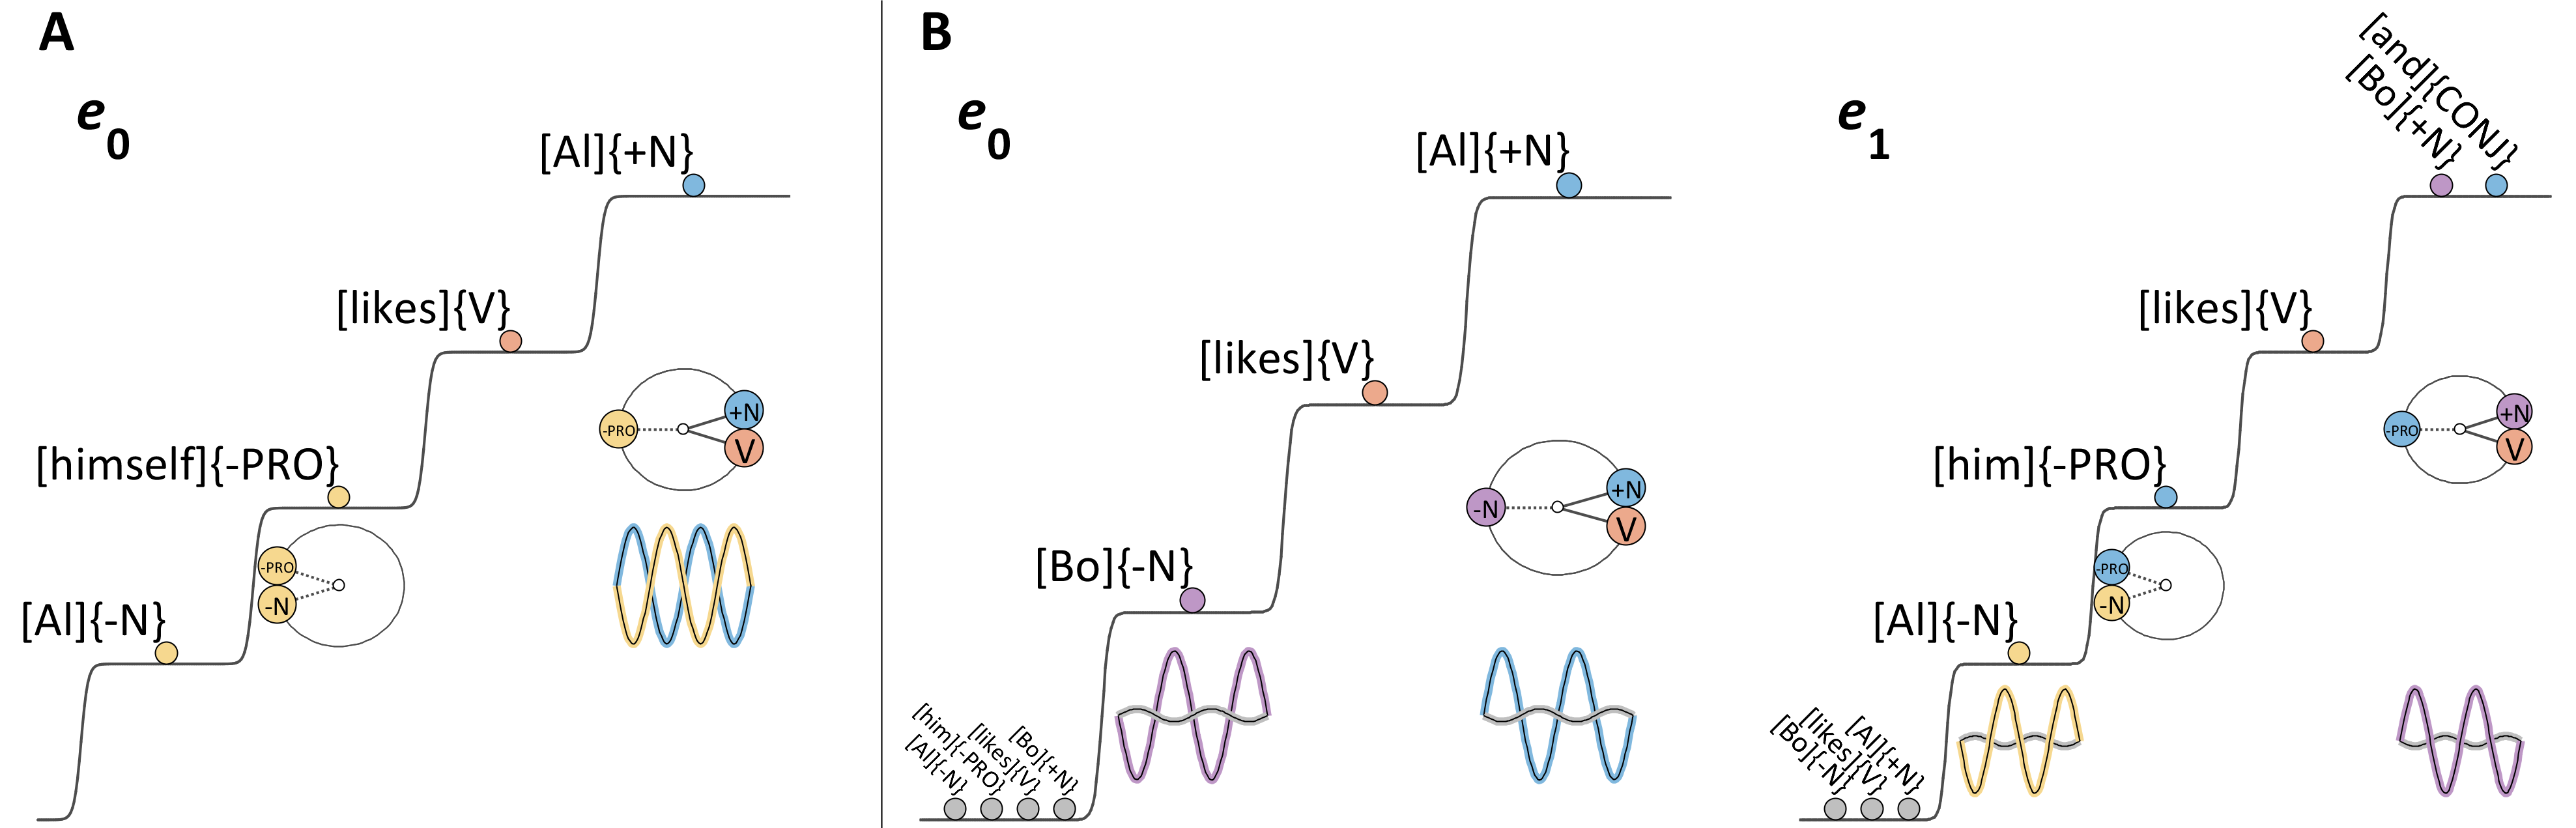
\includegraphics[width=\textwidth]{figures/Tilsen-img156.png}
\caption{\missingcaption}
\label{fig:7:12}
\end{figure}
 

  It is informative to consider a related utterance, \textit{Al likes Al}, which is readily coherent in a contrastive context, e.g. \textit{Al doesnt like Bo. Al doesnt like Cam. Al likes Al}. This also requires destructive c-differentiation of [Al] such that there are [Al]\{+N\} and [Al]\{-N\} systems, but [Al]\{-N\} is typically co-selected with a focus system [\textsc{foc}]\{\textsc{foc}\}. The fact that [\textsc{foc}] or [\textsc{self}] (which we now see as a special type of [\textsc{pro}]) are strongly biased to occur in the destructive c-differentiation context suggests that these systems may serve to stabilize a configuration which is otherwise somewhat unstable.

  The relational meaning experience associated with destructive c-differentiation of \{N\} often takes on an additional flavor. For example, \textit{Al likes himself} may have some idiomatic quality of meaning that differs from \textit{Al likes Bo}, or \textit{Al likes coffee}. The additional idiomatic quality is perhaps more obvious in examples like \textit{Al knows himself, Al kicks himself}, or \textit{Al pushes himself}—all of which induce idiosyncratic meaning experiences which are not readily analyzed as compositional. These special flavors of meaning are difficult to describe, but our conceptual model suggests that they involve alternative patterns of ground-level c-system excitation.

  To further analyze binding phenomena lets consider the examples below where the reflexive form does not readily cohere. Initial configurations for each of these sentences are shown below. One important aspect of the analysis is the hypothesis that \{\textsc{poss}\} s-systems are similar to \{P\} systems in that \{\textsc{poss}\} typically relates two systems, one of which \{\textsc{poss}\} is +φ coupled with, the other it is -φ coupled with. In examples (B) and (C), we see that because of the hypothesized configurations for \{\textsc{poss}\}, the [Al] c-differentiation is not destructive, i.e. the differentiated [Al] systems in fact interfere constructively. Hence the required conditions are not present for use of [\textsc{self}]. 

\ea
\ea[*]{himself\textsubscript{i} likes Al\textsubscript{i}}.
\ex[*]{Al’s friends like himself\textsubscript{i}}.
\ex[*]{Al likes himself’s friends.}
\z
\z

\begin{figure}
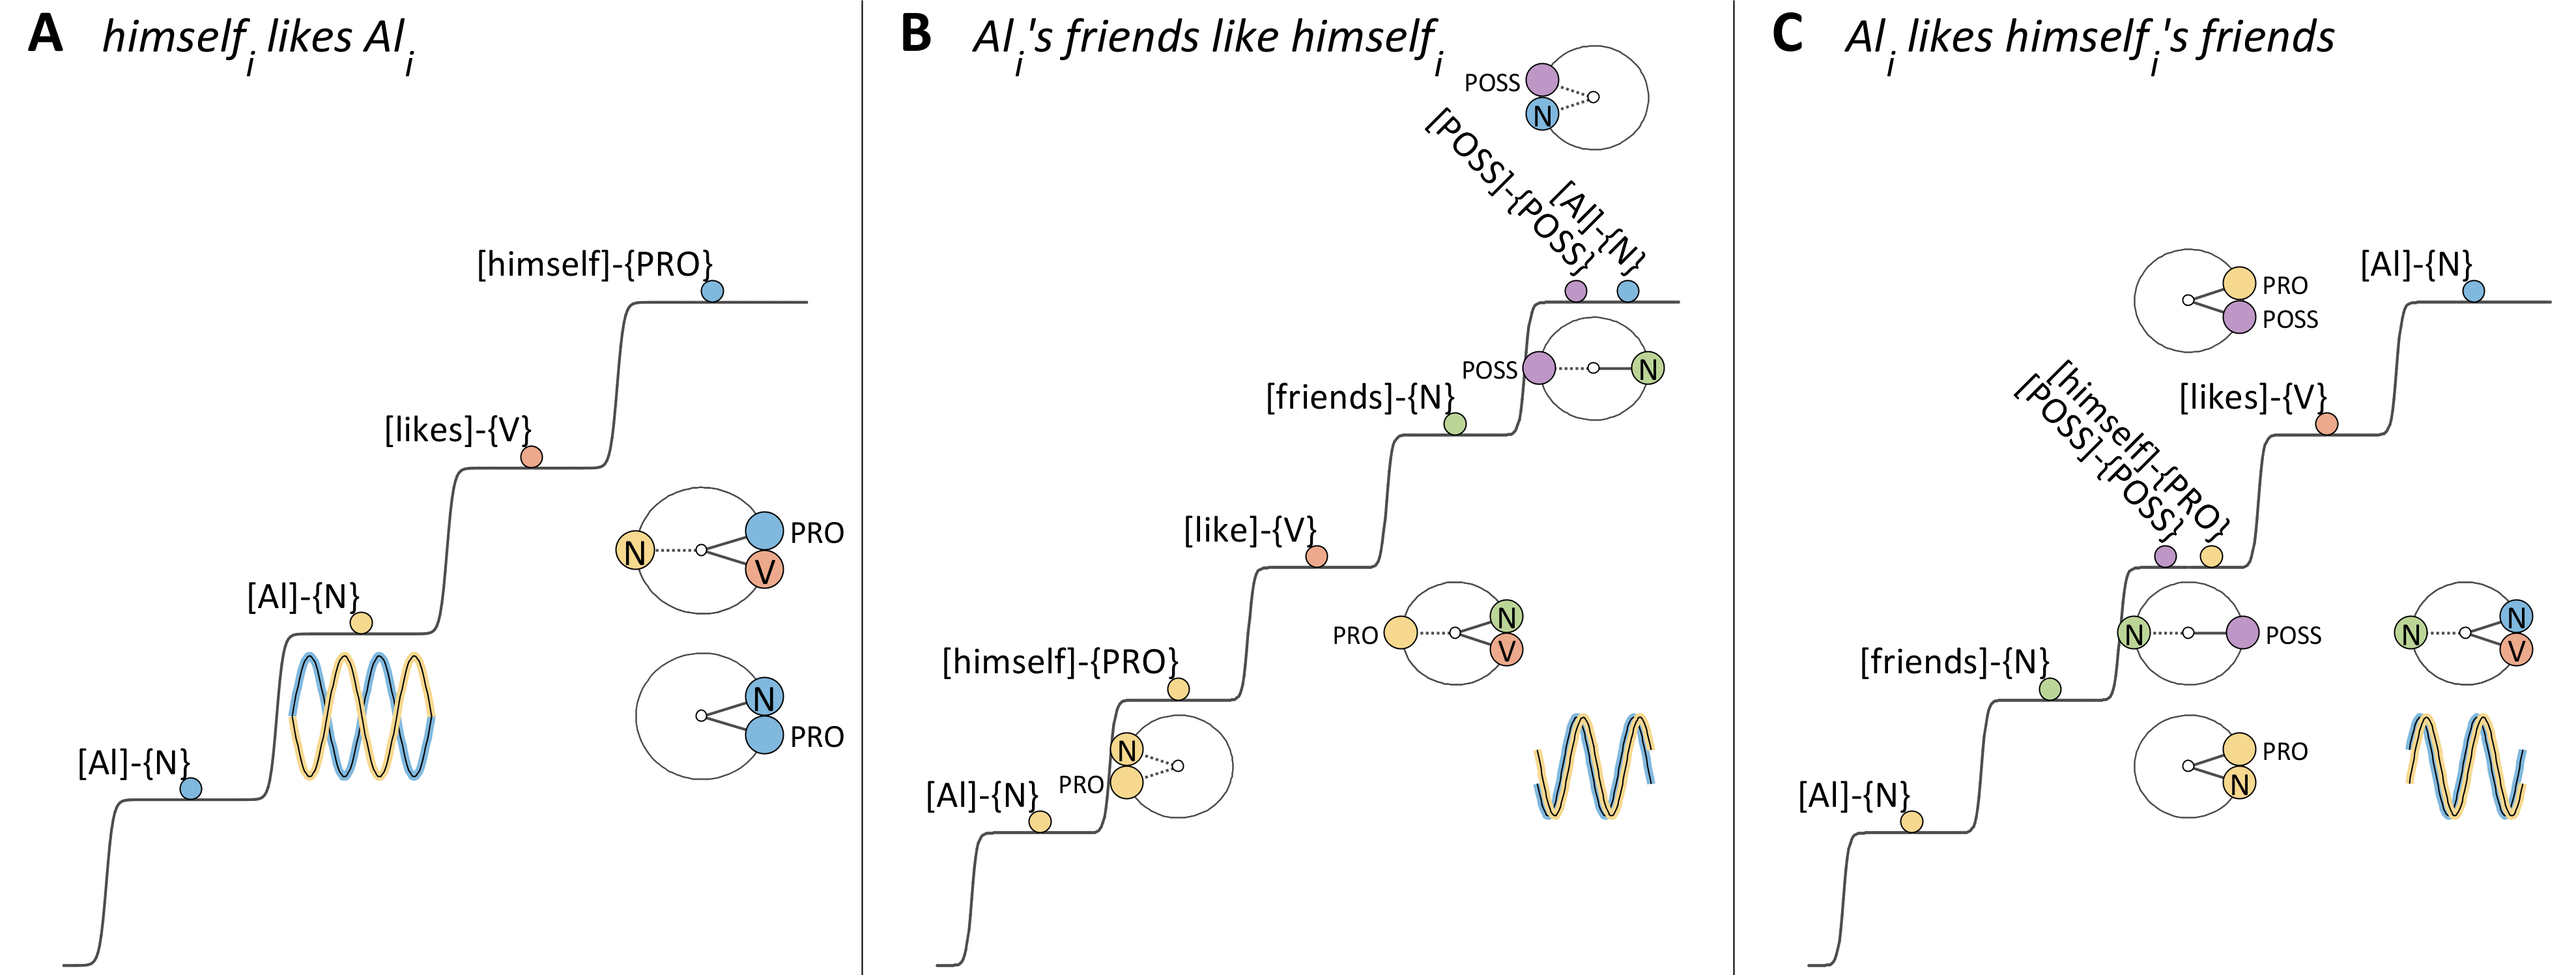
\includegraphics[width=\textwidth]{figures/Tilsen-img157.png}
\caption{\missingcaption}
\label{fig:7:13}
\end{figure}
 

  The analysis of (B) and (C) cannot be extended to (A), where the [\textsc{self}] form is +φ coupled to \{V\}. To explain the noncoherence of (A) a different account is needed. This could involve a number of factors, such as the +φ relation of [\textsc{self}] to \{V\}, its status as clause-initial, and/or its selection before the lexical system [Al]\{N\} to which it is coupled. There are many additional complications in the analysis of self forms which we do not address in detail here (see \citealt{KönigSiemund2000,Safir2004}). Logophoric and emphatic uses of self-forms as in \textit{Al likes the picture of himself} and \textit{Al, himself a coffee-drinker, eats granola} most likely involve a different cs-system than the one we posited above, and this system is not subject to the same constraints as [\textsc{self}]\{\textsc{pro}\}. 

  Although a more comprehensive analysis is still in order, it is reassuring that to conceptualize binding phenomena in the o/el framework, we did not need to invent new mechanisms. Instead, the contexts in which self-forms are obligatory and prohibited correspond fairly well to a particular form of differentiation interference, which is predicted by our model whether or not self-forms are present in a given language. Furthermore, it appears that a general analysis of anaphora can be built upon the very same concepts of grounding vs. non-grounding demotion that are generally useful in the o/el framework.

\section{Wh-questions and islands}

In conventional approaches, a common analysis of question formation in many languages involves an object movement schema (\citealt{Baker1970,Cheng1997,Chomsky1965,Karttunen1977}). For example, the wh-question in (a) is understood to be created by moving the wh-expression in (b). The wh-expression in (b) is in the same position where it would occur in the corresponding declarative utterance (c):

\ea
\ea{What did Al drink?}
\ex{Al drank what?}
\ex{Al drank coffee.}
\z
\z

  Below we construct an o/el understanding of Wh question patterns based on excitation in pre-selective production, similar to the analysis of topicalization. We then extend the account to a variety of so-called island effects, circumstances in which wh-promotion does not readily occur. 

\subsection{Wh-systems and long-distance dependencies}

The first question to address is whether we should pursue an analysis that proliferates s-systems or c-systems, i.e. whether we will construct \{\textsc{whN}\}, \{\textsc{whADV}\}, etc. or [\textsc{wh-nominal}], [\textsc{wh-adverbial}], etc. Observe that wh-forms such as \textit{what}, \textit{who}, \textit{why}, \textit{how}, \textit{where}, etc., when used for questions, have distributions which are similar to those of a variety of s-systems and obtain identical φ-coupling relations to \{V\}. An analysis is possible that proliferates classes of s-systems for these expressions, such as \{\textsc{whN}\}, \{\textsc{whV}\}, \{\textsc{whADJ}\}, and \{\textsc{whADV}\}, but this proliferation is unnecessary. Instead, we view wh-expressions as the gm-domains of a special class of c-systems, which we refer to as \textit{wh-systems.} These wh-systems form cs-resonances with the lexical s-systems that we have already constructed. We thus propose the following configurations for the above examples:

  
\begin{figure}
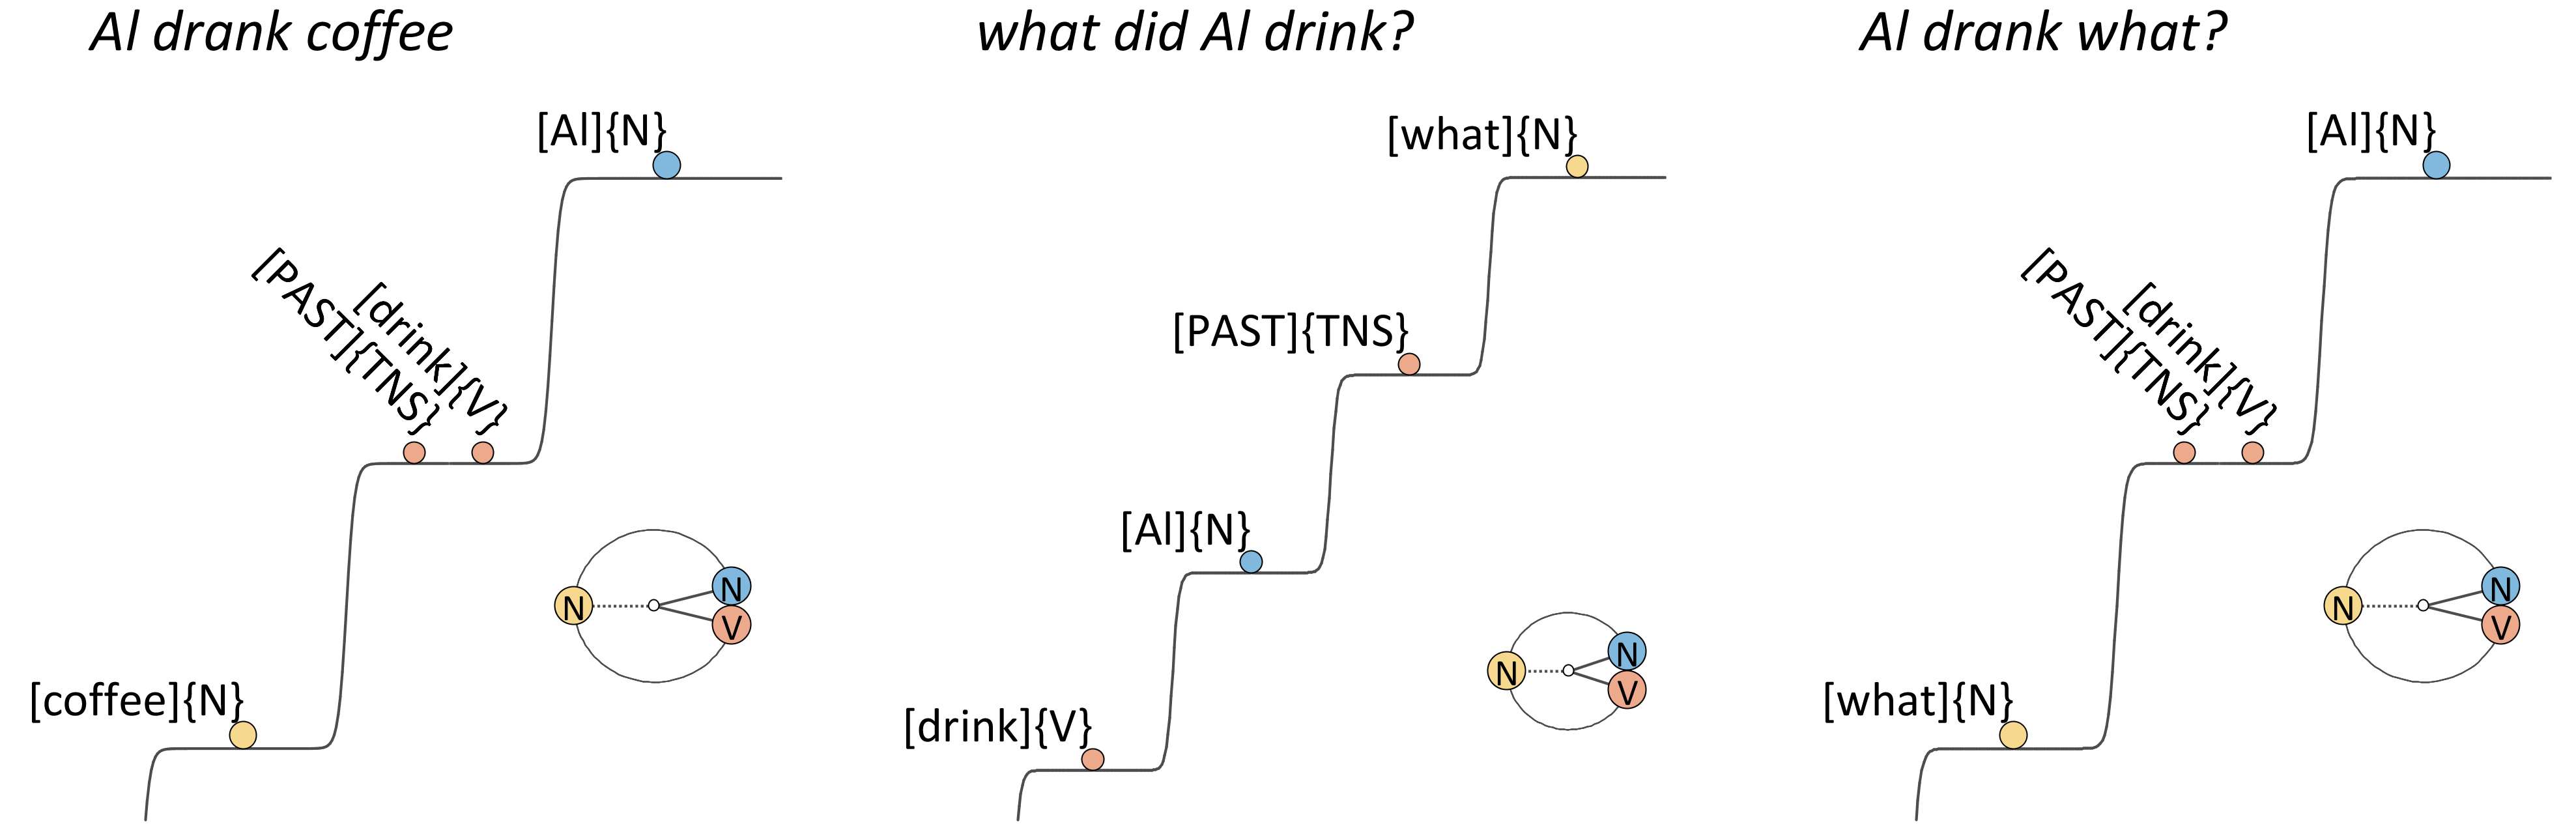
\includegraphics[width=\textwidth]{figures/Tilsen-img158.png}
\caption{\missingcaption}
\label{fig:7:14}
\end{figure}
 

  In support of this approach, we observe that not only does each lexical s-system have a corresponding wh-expression, but for some lexical s-system classes there are several different gm-domains which are associated with different flavors of meaning (cf. the adverbials, as well as person vs. non-person \{N\}). The conceptual specificity of the gm-domains supports the c-system subclass analysis, since in general we do not expect to construct classes of s-systems to accommodate detailed variation in meaning flavors.

\begin{table}
\begin{tabularx}{\textwidth}{XXX}
\lsptoprule
\{N\} & [Wh-N] & \textit{what}\\
\{N\} (people) & [Wh-person] & \textit{who}\\
\{V\} & [Wh-V] & \textit{what}\\
\{Adj\} & [Wh-Adj] & \textit{what}\\
\{Adv\} (manner) & [Wh-manner] & \textit{how}\\
\{Adv\} (reason) & [Wh-manner] & \textit{why}\\
\{Adv\} (temporal) & [Wh-time] & \textit{when}\\
\{Adv\} (location) & [Wh-loc] & \textit{where}\\
\{Dem\} & [Wh-demonstrative] & \textit{which}\\
\lspbottomrule
\end{tabularx}
\caption{\missingcaption}\label{tab:7:4}
\end{table}
  Wh-systems are hypothesized to have relatively weak interactions with sensory-motor surroundings, compared to prototypical c-systems. Recall that prototypical c-systems, on the microscale, are distributed populations that interact with diverse sensory and motor systems. For example, [coffee] is associated with the smell of coffee, its taste, its temperature, what it looks like, the sound of it brewing, steam coming off of it, etc.; various episodic memories associated with coffee: brewing it in different contexts, buying it, spilling it, etc.; various motor memories: how to hold a cup of it, how to drink it, etc. Prototypical lexical c-systems have many such associations, and we conceptualize these as interactions with sensory and motor systems. In contrast, we hypothesize that wh-systems lack strong interactions with the surroundings. Of course, wh-systems do not lack surroundings interactions entirely: semantic differences such as person/animate from non-person/non-animate (\textit{who} vs. \textit{what}) can differentiate wh-systems. But the semantic differentiation of wh-systems is evidently more generic.

  Furthermore, we conjecture that the wh-system population sizes are relatively large and/or more distributed compared to prototypical lexical c-systems. One consequence of this is that there is more internal interference in a wh-system than in a prototypical c-system, and this makes prototypical c-systems likely to outcompete wh-systems for excited cs-resonances. We can also view wh-systems as super-populations, overlapping with large numbers of c-systems. For example, all nominal concepts (i.e. c-systems which couple to \{N\}) might share a [whN] subpopulation that couples to \{N\}. This implies that when a c-system such as [coffee] is activated, the c-system [what]\{N\} would also be activated, but [coffee] typically outcompetes [whN] for cs-resonance. When no specific c-systems (such as [coffee] or [tea]) experience strong surroundings forces, then perhaps the corresponding wh-system [whN] is more likely to become excited.

  Another consequence of the population size/spread conjecture is that when wh-systems do form excited cs-systems, the \textit{e} values of those systems will be relatively high. This provides a potential explanation for why wh-systems have a tendency to be promoted to selection-level in initial e configurations: the relatively high \textit{e} values of wh-systems augments the \textit{e} value of the corresponding cs-system in the pre-stable organization phase. Relatedly, wh-systems are often co-selected with a \{\textsc{focus}\} s-system, i.e. [\textsc{question}]\{\textsc{focus}\}, which is similar to [\textsc{contrast}]\{\textsc{focus}\} and may further augment excitation.

  
\begin{figure}
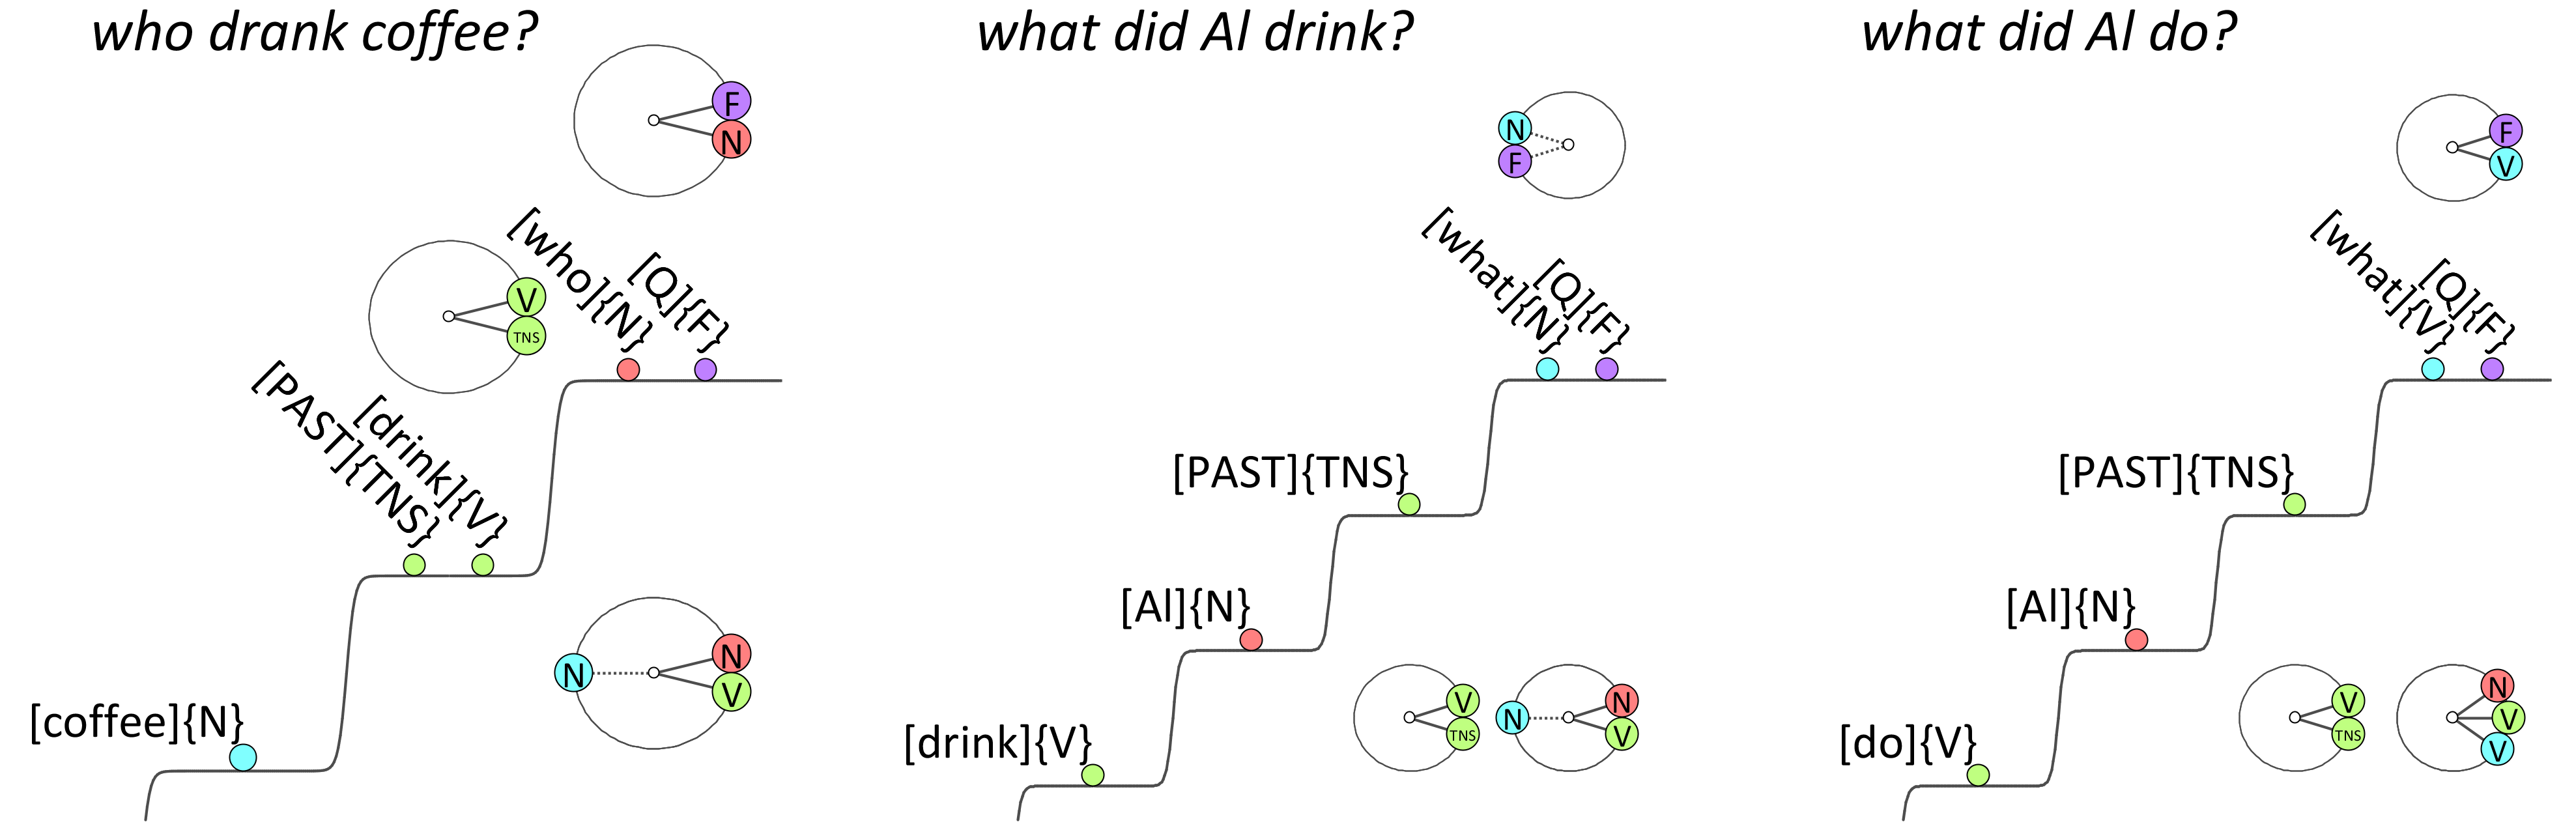
\includegraphics[width=\textwidth]{figures/Tilsen-img159.png}
\caption{\missingcaption}
\label{fig:7:15}
\end{figure}
 

  The activation of a wh-system and [Q] (i.e. [\textsc{question}]) normally results in an initial configuration in which the wh-system is promoted to selection level through augmented excitation. However, promotion does not inevitably occur from augmented excitation, as shown by echo questions, i.e. \textit{Al drank WHAT?} and Wh in-situ, i.e. \textit{Who drank what?} Note that many conventional analyses require movement of in-situ wh-forms in a semantic representation (i.e. logical form), because the relevant meaning relations must be viewed as patterns of connection (see \citealt{Reinhart1998,Watanabe1992}).

  Another question pattern to consider is one in which no particular wh-system is excited, i.e. yes-no questions. In such cases, lexical cs-systems are selected and the meaning experience involves questioning a clausal set of φ configurations. In the examples below, the {\textbar}Al drank coffee{\textbar} configuration is questioned. In this case there is no wh-system to promote, and promotion of \{\textsc{tense}\} with \textit{do}{}-support occurs instead. The noncoherence of in situ utterances with \{\textsc{tense}\} promotion (i.e. *\textit{Al did drink what?}) suggests that \{\textsc{tense}\} promotion is a consequence of promotion of [\textsc{q}]\{\textsc{focus}\} and/or promotion of [\textsc{wh}]\{N\}. 

  
\begin{figure}
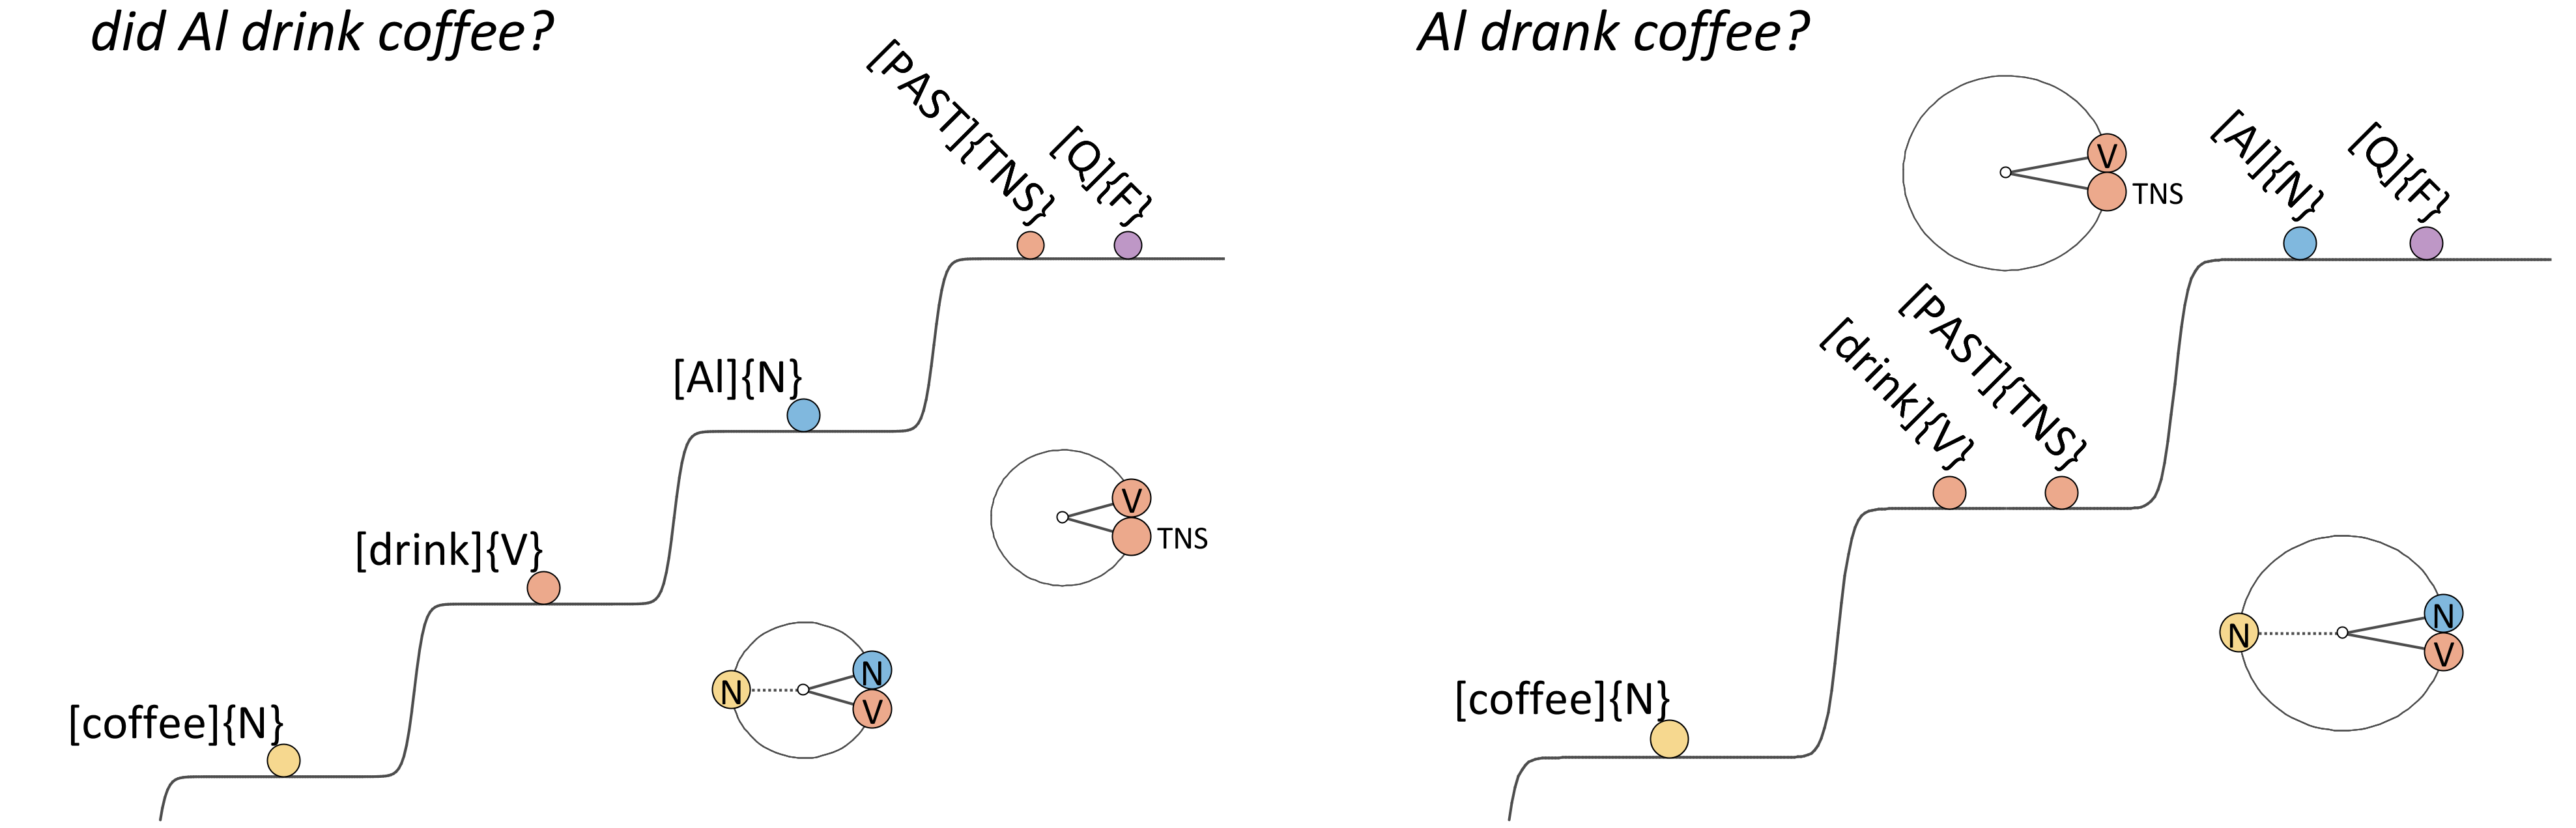
\includegraphics[width=\textwidth]{figures/Tilsen-img160.png}
\caption{\missingcaption}
\label{fig:7:16}
\end{figure}
 

  Further support for the connection of \{\textsc{tense}\} promotion with [\textsc{q}]\{\textsc{focus}\} promotion comes from the non-coherence of \{\textsc{tense}\} promotion when the subject NP is questioned, as shown below in (a) and (b). In these utterances, neither [Q]\{\textsc{focus}\} nor [\textsc{wh}]\{N\} are promoted from augmented excitation—[wh]\{N\} already occupies the initial selection level because of learned φ-e mappings. Note that \textit{do}{}-support for [\textsc{tense}] systems should be distinguished from emphatic \textit{do} in \textit{Al did drink coffee} and the corresponding question in (c).  

\ea
  \ea[]{Who drank coffee?} 
  \ex[*]{Who did drink coffee?}
  \ex[]{Who DID drink coffee?}
  \z
\z

  In the o/el conceptualization, wh-question patterns involve promotion of a wh-system in the pre-stable organization phase. Whether this promotion occurs is determined by the surroundings forces. The [\textsc{Q}]\{\textsc{focus}\} system we have posited can be interpreted as a manifestation of the relevant surroundings states. Moreover, from the coherence of (c) and multiple-wh utterances such as \textit{who drank what?} we infer that [Q]\{\textsc{focus}\} can occur at most once with each set of co-selected systems. This reinforces the notion that [Q]\{\textsc{focus}\} and [\textsc{contrast}]\{\textsc{focus}\} have a deep similarity, based on their pragmatic origins and manifested in their propensity to couple with the accentual s-system, \{\^{}\}. Recall that \{\^{}\} is special by virtue of its association with the selection level of an e-potential. One possibility we leave for future consideration is whether in some question trajectories [Q]\{\textsc{focus}\} is re-promoted to selection level with each re-organization; an analysis of this sort could account for the intonational patterns associated with yes/no questions and clausal contrast.

   The o/el conception is not consistent with any object-metaphor conception in which word-objects move from one position to another. A conventional justification for a structural notion of movement involves the concept of a \textit{trace} (a phonologically “empty” syntactic object, cf. \citealt{Chomsky1965}), which could be interpreted in the o/el framework as a cs-system without a gm-domain. To assess this, lets consider the non-coherence of the utterances below.

\ea
  \ea[*]{Who Al drank coffee?}
  \ex[*]{What did Al drink coffee?}
\z
\z

  How do we account for the non-coherence of (b), where [what] and [coffee] c-systems are excited?  We could stipulate that a [\textsc{trace}]\{N\} system is excited and coupled to \{V\}, as shown below in (A). However, this is not necessary in the o/el framework. The non-coherence of (b) follows straightforwardly from our configurational invariance hypotheses. A transitive \{V\} system such as [drink]\{V\} +φ couples to one agentive \{N\} system and -φ couples to one patientive \{N\} system. In the initial configuration of example (b) shown in (B) below, [coffee]\{N\} has no lexical \{V\} system to couple to (because [drink]\{V\} is already coupled with [what]\{N\}), and thus the epoch is non-coherent.

  
\begin{figure}
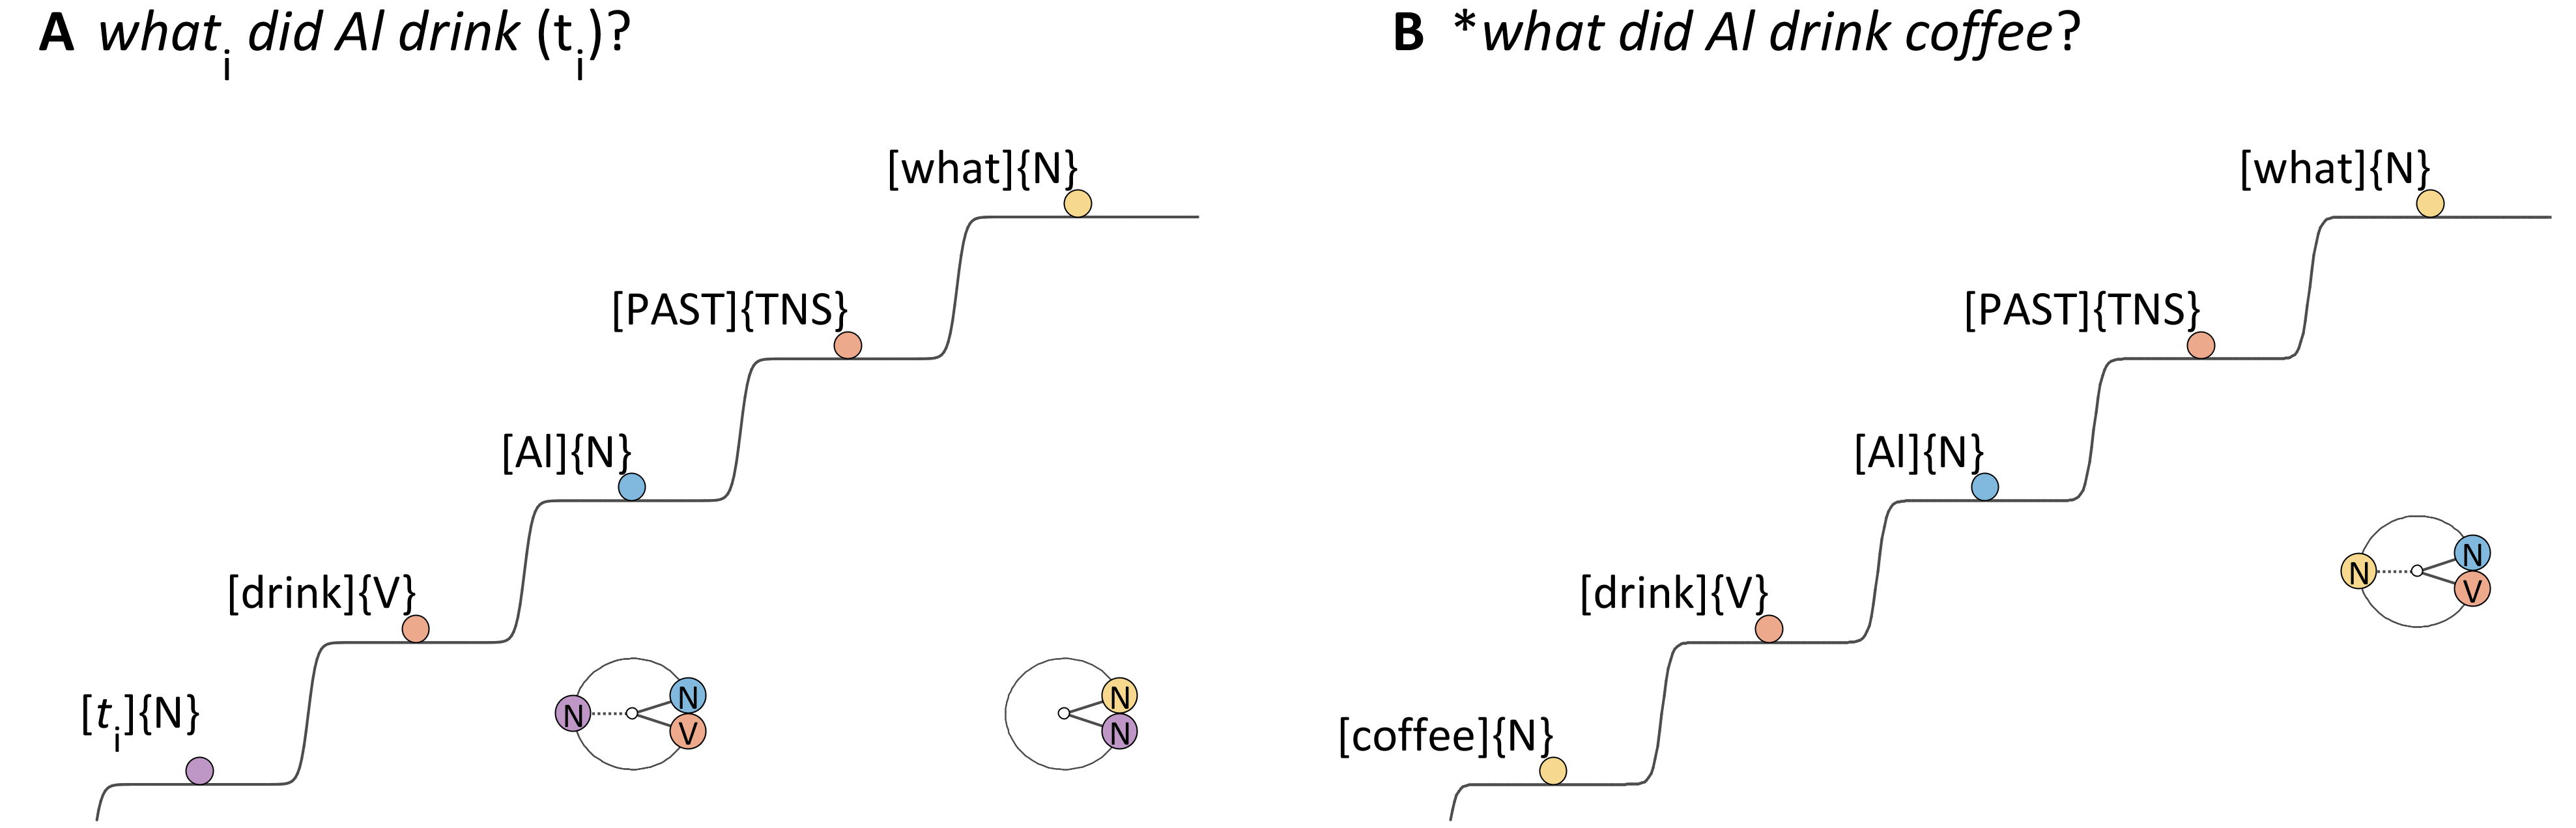
\includegraphics[width=\textwidth]{figures/Tilsen-img161.png}
\caption{\missingcaption}
\label{fig:7:17}
\end{figure}
 

  The trace account in (A) is also problematic because e-levels are only organized for cs-systems with a gm-domain. In all other analyses, cs-systems with no gm-domain are co-organized with some cs-system which has a non-empty gm-domain. This condition can be interpreted as a consequence of the accentuation hypothesis whereby each set of co-selected cs-systems can excite at most one accentual s-system \{\^{}\}—\{\^{}\} is viewed as a consequence of selection, rather than a syntactic-conceptual resonance. Furthermore, recall that in languages with stress, \{\^{}\} manifests as a primary stress/accent in gm-organization. Because systems with empty gm-domains (such as a hypothetical [\textsc{trace}]\{N\} system) cannot be stressed, the trace analysis shown above is untenable.

  One interesting characteristic of wh-systems promoted through augmented excitation in the question context is their propensity to persist in an excited state throughout a series of clausal reorganizations. Depending on the type of reorganization that occurs, a [\textsc{wh}] c-system can remain above ground instead of being demoted to ground. This behavior accounts for so-called “unbounded dependencies” associated with wh-expressions. An example trajectory is shown below. The [what]\{N\} and [Q]\{\textsc{focus}\} systems remain above ground throughout the entire trajectory, even after the complement clause reorganization Ê\textsubscript{5}. Coupling to  [Q]\{\textsc{focus}\} assists the persistence of [wh]\{N\} excitation, in the same way that \{\textsc{aux}\} assists persistent excitation of \{V\} in ellipsis. 

  \ea
    {What does Bo know that Al drinks?}
\z
  
\begin{figure}
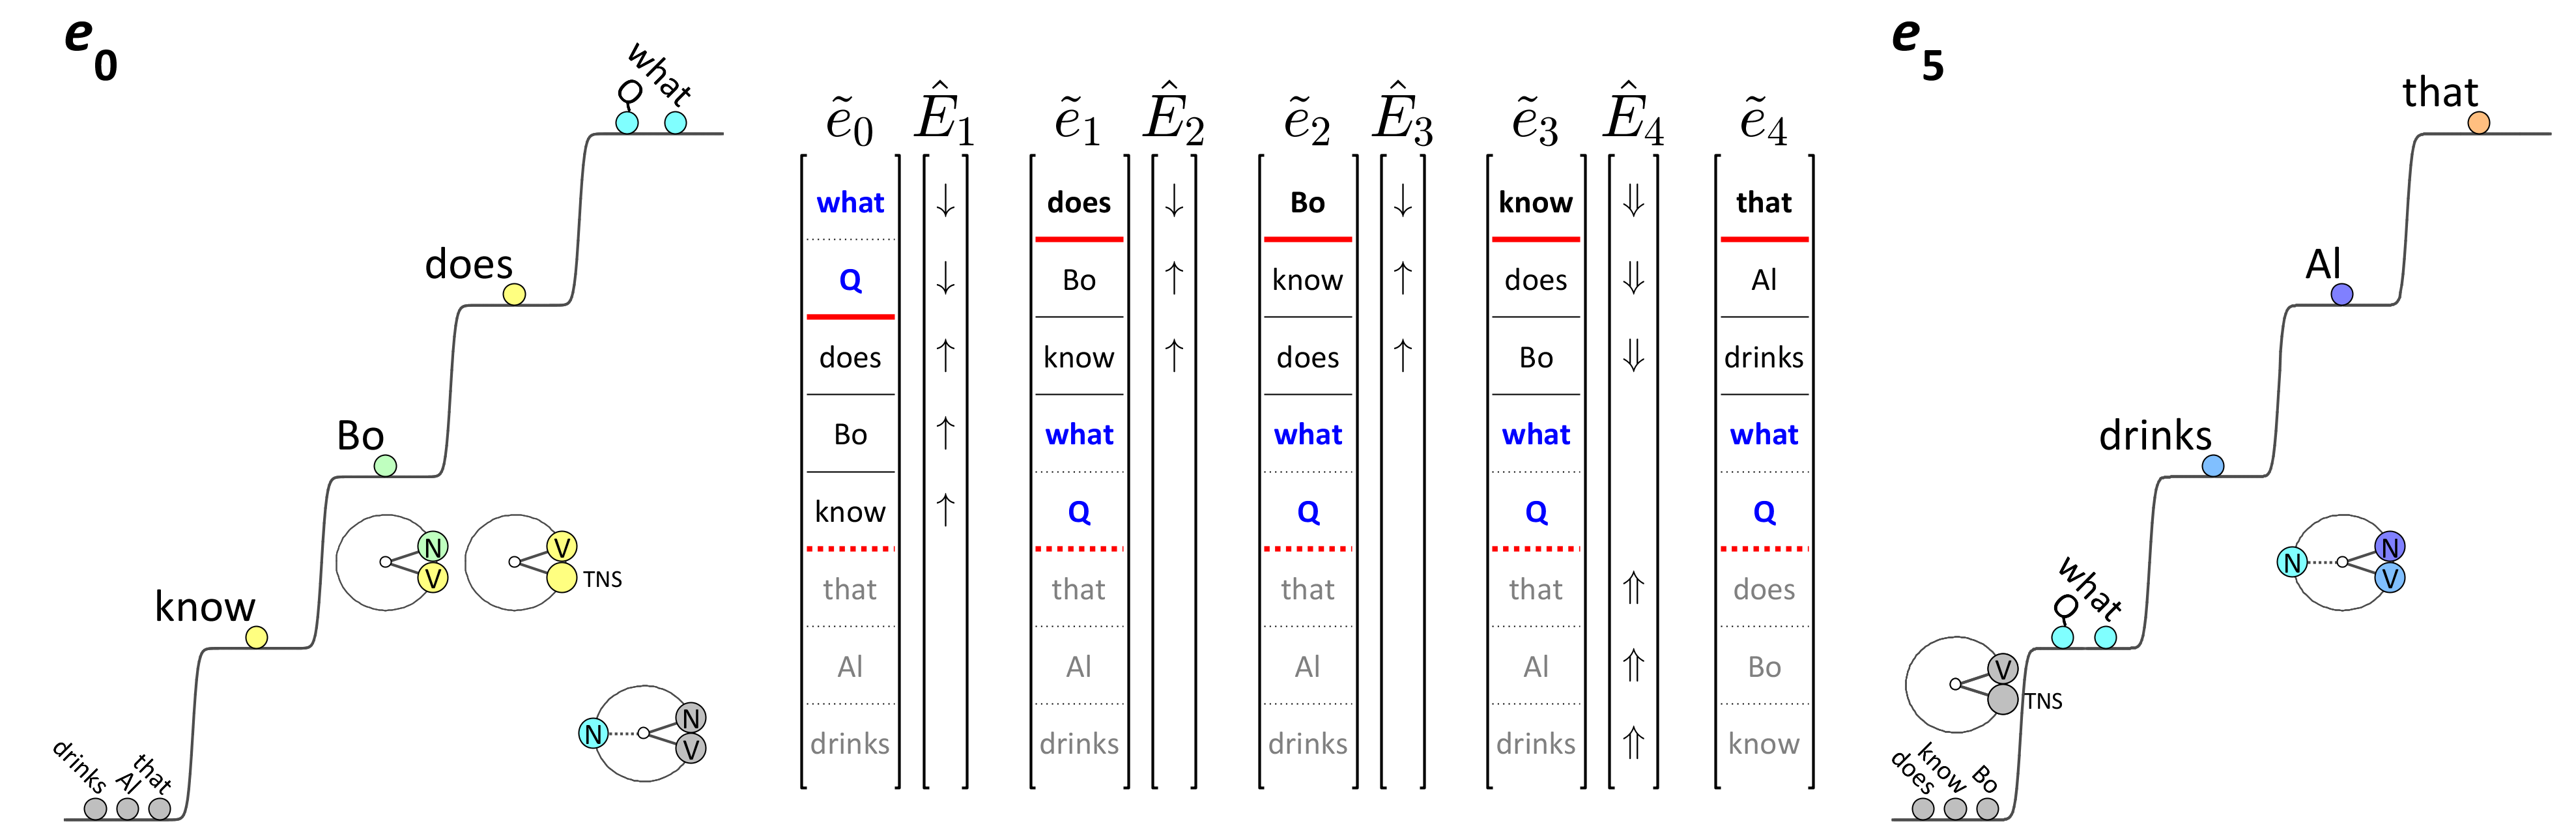
\includegraphics[width=\textwidth]{figures/Tilsen-img162.png}
\caption{\missingcaption}
\label{fig:7:18}
\end{figure}
 

  In the o/el picture, long distance wh-dependencies are trajectories in which a [wh] system coupled with [Q] remains excited through a reorganization which grounds unattended systems (typically of a clause). However, not all clausal reorganizations allow for persistent excitation: there are a number of reorganizations in which grounding forces outweigh persistent excitation. This results in so-called island phenomena \citep{Ross1967}.

\subsection{Islands}

The analysis of island phenomena we develop here proposes two different mechanisms for islands. We examine only a subset of island types, and our aim is fairly modest: to provide a starting point for a more comprehensive theory. The first mechanism applies to cases in which a φ configuration cannot cohere because the relevant [wh] system is grounded by an intervening reorganization, rather than persisting in an excited state. This applies to adjuncts, wh-clauses, and relative clauses, which are exemplified below. In contrast, \textit{that} complement clauses and bare complements do not strongly ground, and hence do not give rise to island effects.

\begin{table}
\begin{tabularx}{\textwidth}{lQQ}
\lsptoprule
\multicolumn{3}{c}{\textbf{Strongly grounding reorganization: island effects}}\\
\midrule
adjunct island & \textit{Bo is mad because Al drinks coffee.} & \textit{*What is Bo mad because Al drinks?}\\
wh-island & \textit{Bo knows why Al drinks coffee.} & \textit{*What does Bo know why Al drinks?}\\
relative island & \textit{Bo knows a story that Al drank coffee} & \textit{*What does Bo know a story that Al drank?}\\
\tablevspace
\multicolumn{3}{c}{\textbf{Non-grounding reorganization: no island effects}}\\
\midrule 
& \textit{Bo knows (that) Al drank coffee} & \textit{What does Bo know that Al drank?}\\
& \textit{Bo wants (for) Al to drink coffee} & \textit{What does Bo want Al to drink?}\\
\lspbottomrule
\end{tabularx}
\caption{\missingcaption}\label{tab:7:5}
\end{table}

  An example trajectory is shown below. The adjunctive reorganization Ê\textsubscript{4} is strongly grounding. Hence [what]\{N\} is grounded by Ê\textsubscript{4}, and the configuration in (e4) does not cohere because not all of the systems in the relevant φ configuration ({\textbar}Al drinks what{\textbar}) are excited. With some effort, [what]\{N\} can be made to persist above ground through Ê\textsubscript{4}, despite this adjunctive reorganization being a strongly grounding one. “Effort” of this sort is almost always a relevant source of variation in coherence intuitions for islands, and in the following section we examine how persistence can account for “exceptions” to the island patterns described here.

  
\begin{figure}
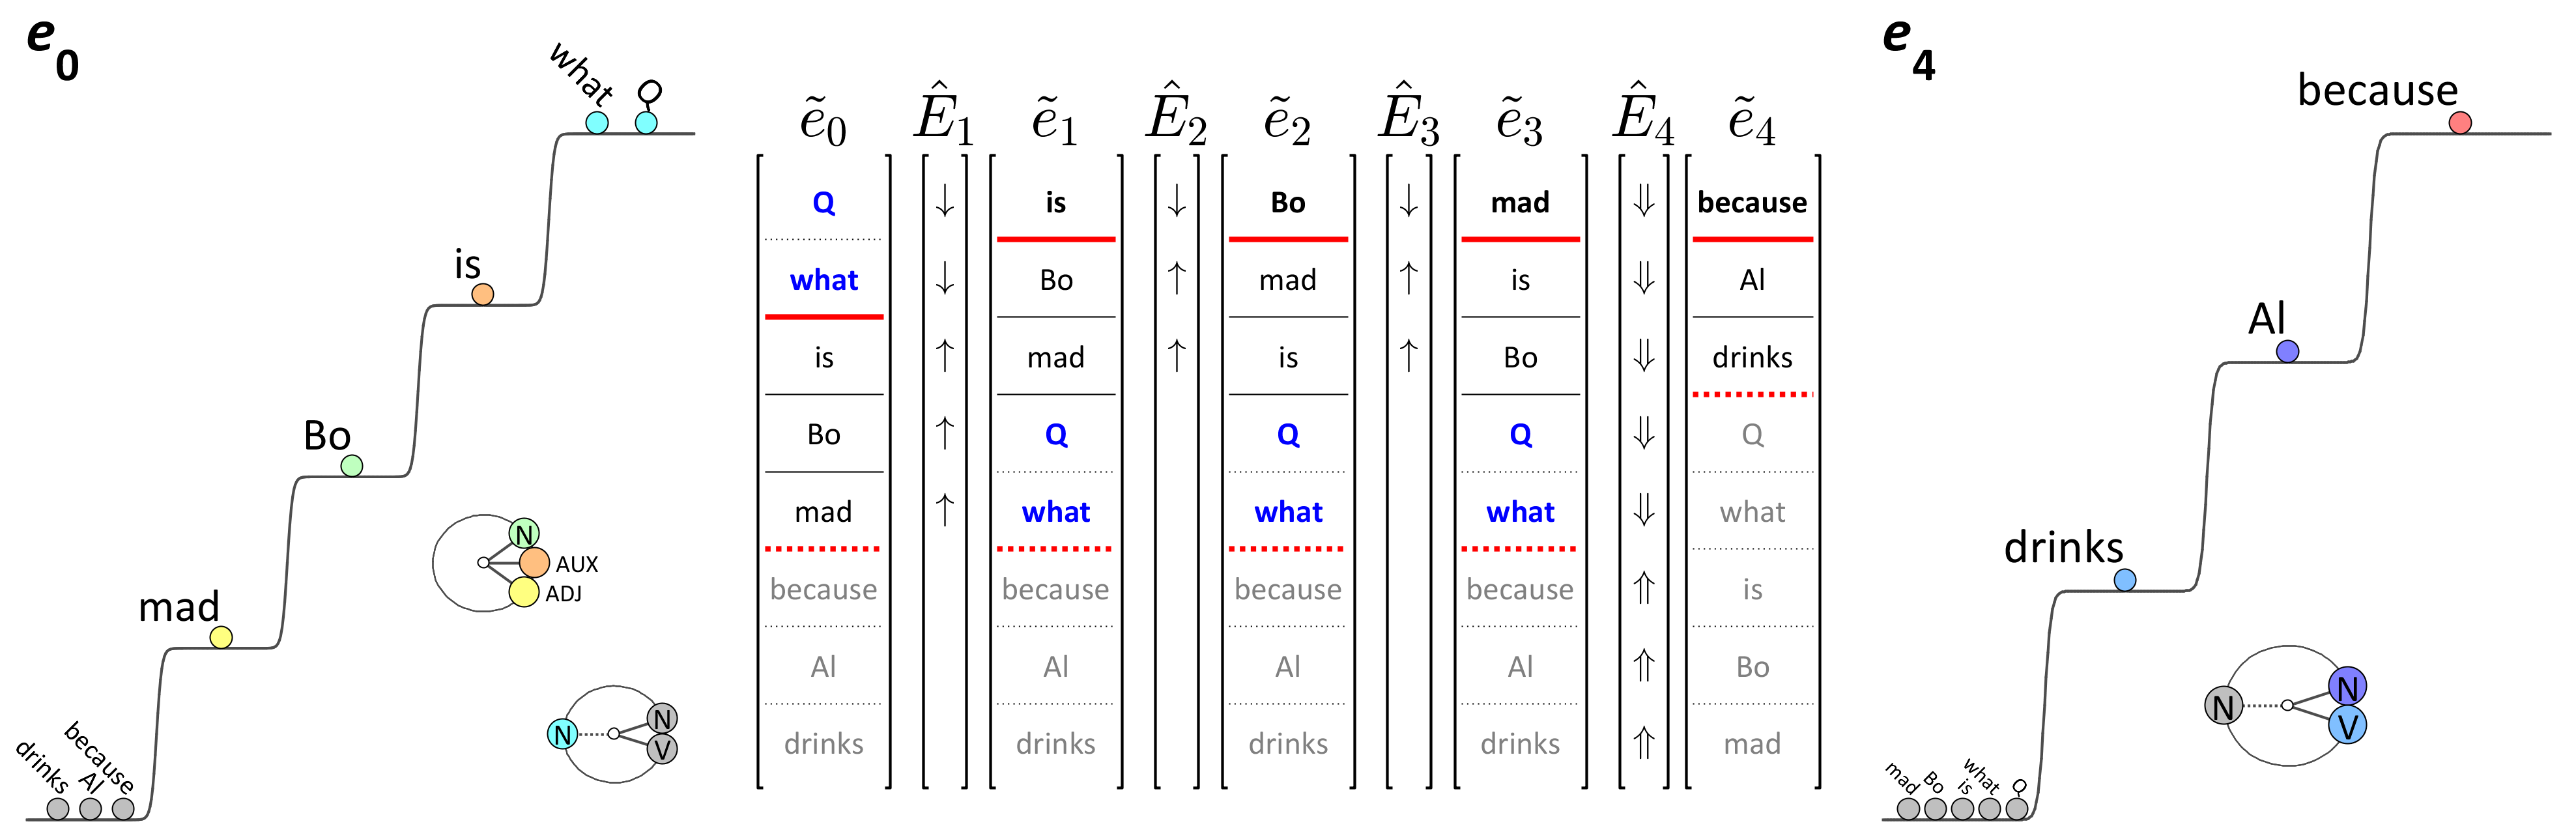
\includegraphics[width=\textwidth]{figures/Tilsen-img163.png}
\caption{\missingcaption}
\label{fig:7:19}
\end{figure}
 

  We can apply the same analysis of strongly grounding reorganization to wh- and relative islands, shown by the trajectory below. Note that the [why]\{ADV\} system is adverbial and hence +φ coupled to [drinks]\{V\}:

  
\begin{figure}
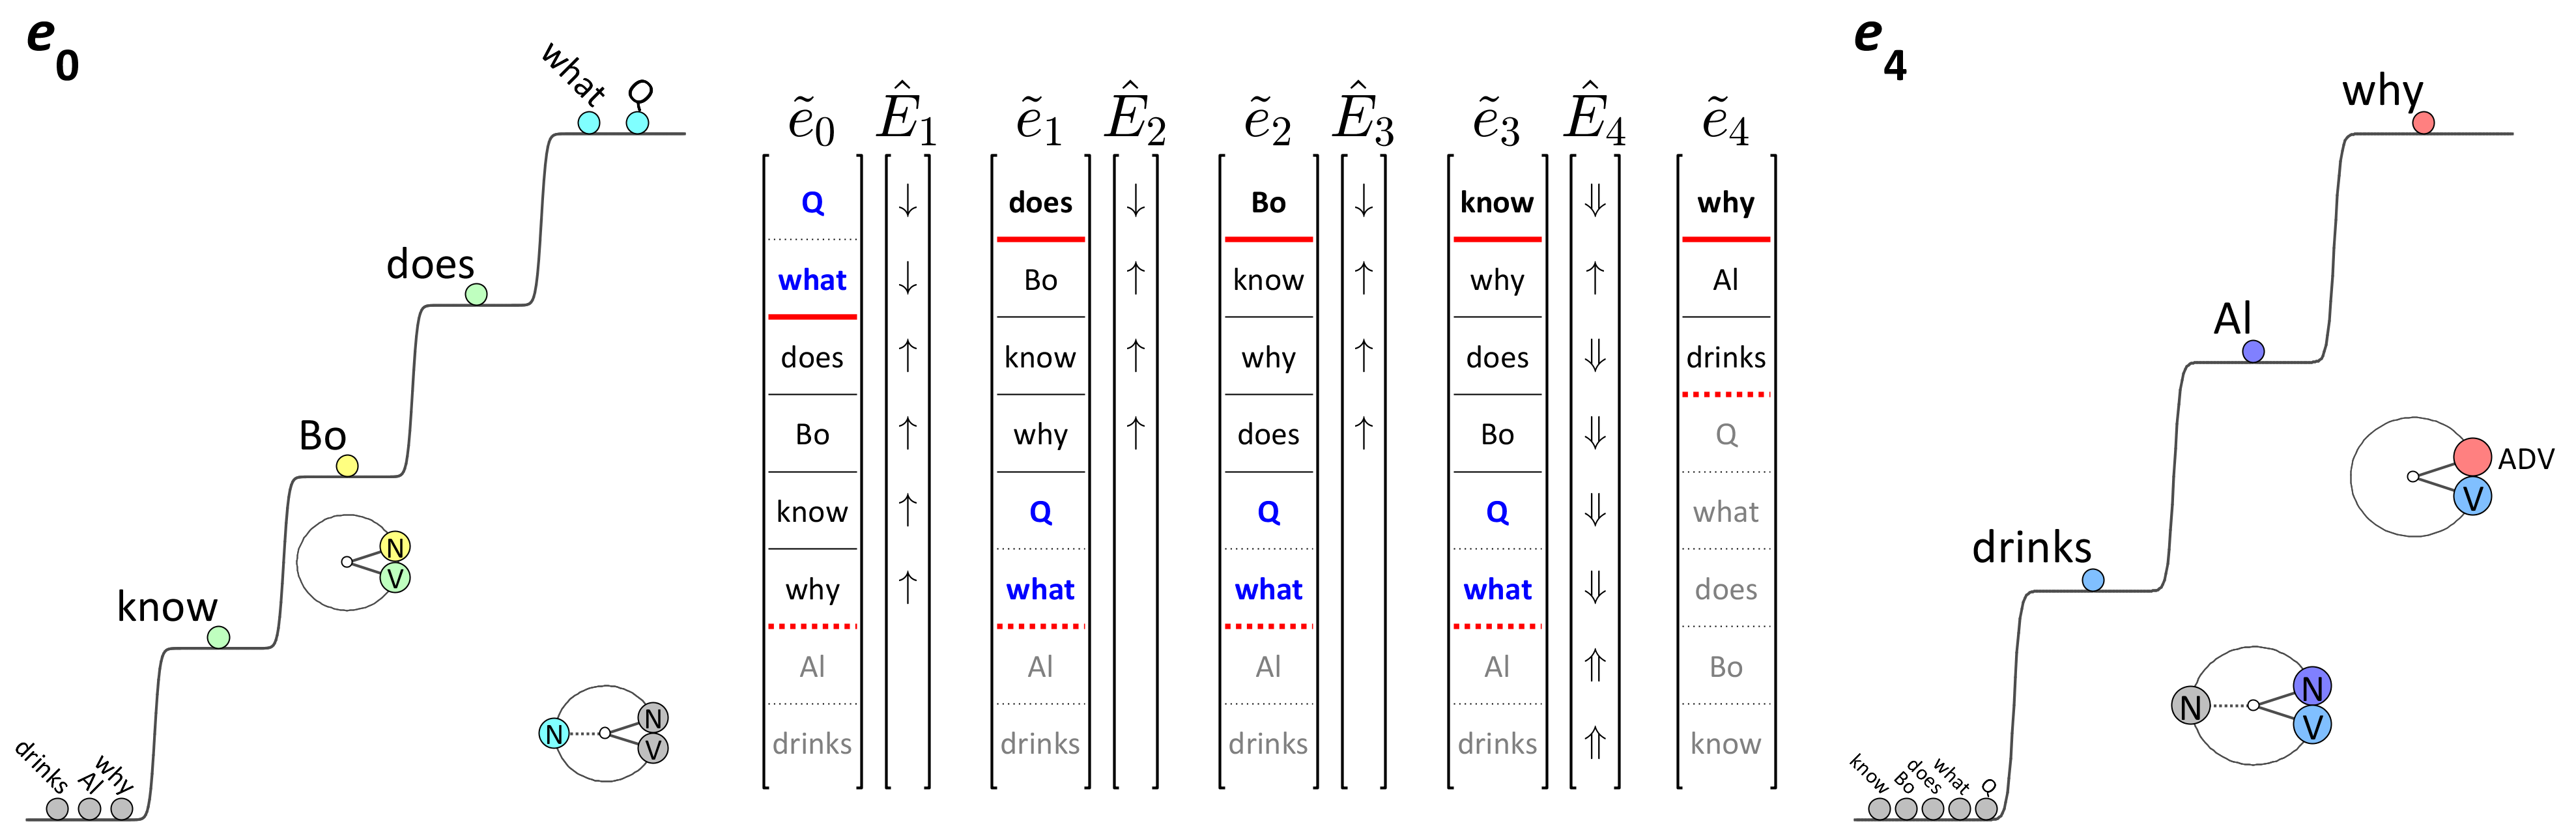
\includegraphics[width=\textwidth]{figures/Tilsen-img164.png}
\caption{\missingcaption}
\label{fig:7:20}
\end{figure}
 

  In contrast to the strongly grounding reorganizations, reorganizations to complement clauses (a), bare nonfinite clauses (b), and clauses of the sort in (c) are weakly grounding:

  \ea
  \ea \textit{What does Bo know that Al drinks?}
\ex \textit{What does Bo want Al to drink?}
\ex  \textit{What does Bo make Al drink?}
\z
\z

  One noteworthy point regarding the difference between strongly and weakly grounding reorganizations is that the cs-systems which are associated with strongly grounding reorganizations, i.e. \textit{because}, \textit{if}, \textit{whether}, \textit{when}, etc., typically have non-empty gm-domains. In contrast, [that]\{C\} is often produced with an empty gm-domain, and bare clause reorganization by definition has no such systems. This suggests that strongly grounding reorganizations are associated with an ungrounding promotion which creates an independent e-level and which contributes additional meaning by virtue of the cs-system that occupies it; weakly grounding reorganizations do not have these qualities.

  Coordination of cs-systems which belong to the same class of s-system, or of configurations of cs-systems which belong to the same s-system classes, allows for persistent excitation, as shown in the (a) examples below. However, when this “coordinate structure” constraint is violated, as in the (b) and (c) examples, we observe island effects. As we argue below, the non-coherence of wh-questions in the above cases is due to violation of configurational hypotheses.

\begin{table}
\begin{tabularx}{\textwidth}{lQQQ}
\lsptoprule
& 1. N coordination

\textit{Al drinks coffee and tea} & 2. VP coordination

\textit{Al drinks coffee and eats granola.} & 3. Clausal coordination

\textit{Al drinks coffee and Bo eats granola.}\\
\midrule 

\textit{a.} & \textit{What does Al drink?} & \textit{What does Al drink and eat?} & \textit{What does Al drink and Bo eat?}\\
\textit{b.} & \textit{*What does Al drink coffee and?} & \textit{*What does Al drink coffee and eat?} & \textit{*What does Al drink coffee and Bo eat?}\\
\textit{c.} & \textit{*What does Al drink and tea?} & \textit{*What does Al drink and eat granola?} & \textit{*What does Al drink and Bo eat granola?}\\
\lspbottomrule
\end{tabularx}
\todo[inline]{This should probably not be a table}
\caption{\missingcaption}\label{tab:7:6}
\end{table}

The coherence of the (a) examples is predicted by our analysis of coordinative reorganizations in ellipsis. Coordinative reorganizations—whether clausal or subclausal—do not demote to ground a cs-system if that system has no corresponding lexical competitor which is promoted from ground. In other words, coordinative reorganizations are not grounding. For example \REF{ex:7:2a} we picture the following trajectory. Both [Al]\{N\} and [what]\{N\} persist in an excited state through the coordinative reorganization Ê\textsubscript{4} because no competitors for these systems are promoted from ground.

  
\begin{figure}
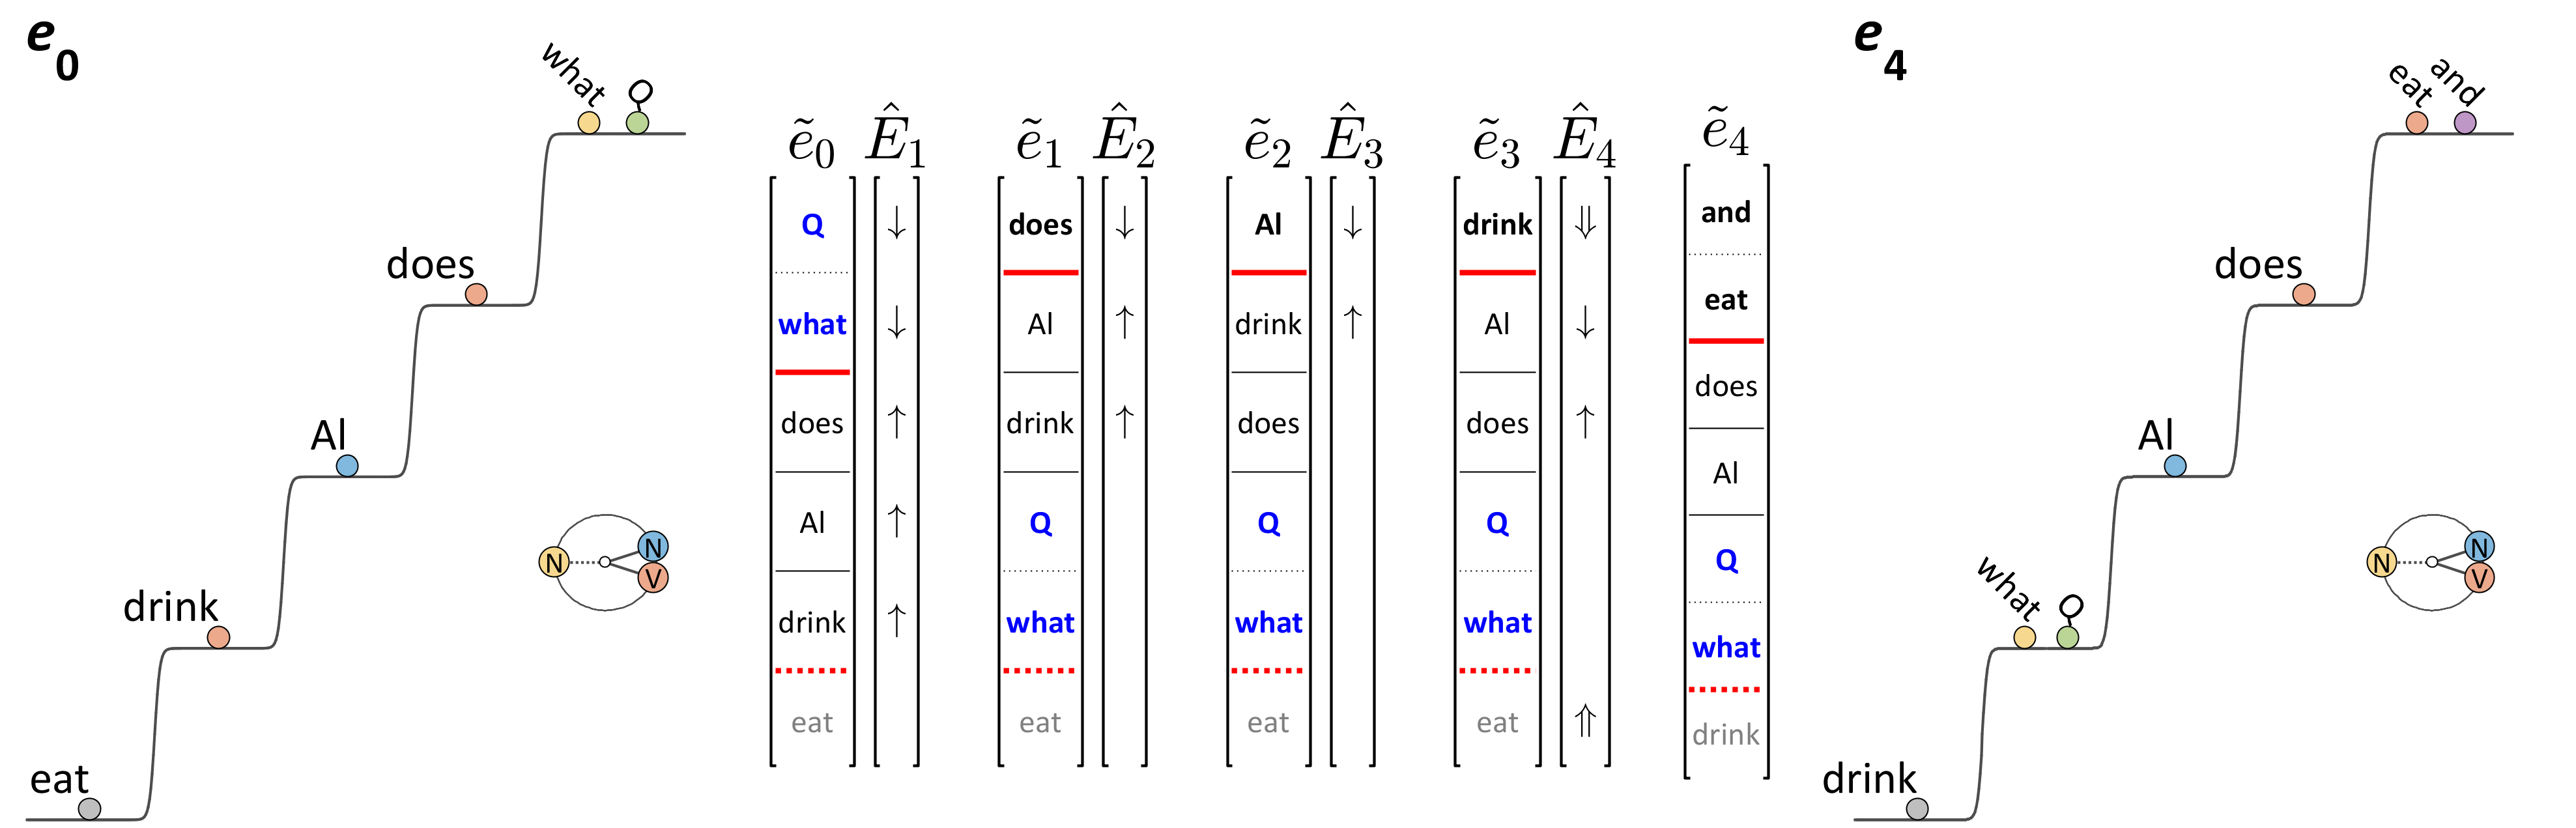
\includegraphics[width=\textwidth]{figures/Tilsen-img165.png}
\caption{\missingcaption}
\label{fig:7:21}
\end{figure}
 

  There are various possible explanations for the non-coherence of the (b) and (c) examples. In the (b) examples, [coffee]\{-N\} interferes with [what]\{-N\} in the epochs before selection of [and]. Furthermore, given our analysis of [and]\{\textsc{conj}\} as a system which becomes excited only upon ungrounding of another system, the (b) utterances should be non-coherent because the selection of [and]\{\textsc{conj}\} does not co-occur with promotion of another system. For example, in \REF{ex:7:1b}, when [and]\{\textsc{conj}\} is promoted to selection, there is no system which it is promoted with. The non-coherence of the (c) examples is more challenging to explain from a production perspective; however, from the perspective of interpretation, it seems likely that an interpreter would couple [what]\{N\} to [drink]\{V\} and ground the entire configuration, leaving the remaining cs-systems unable to cohere.

Another mechanism for island effects relates to circumstances in which one of set of coupled lexical systems is promoted initially with augmented excitation. For example, when an \{ADJ\} or \{POSS\} modifier is coupled to \{N\}, promotion of the modifier to selection level in the initial configuration prevents coherence. Examples \REF{ex:7:1a}-(1d) below illustrate the island patterns. Note that a strongly grounding reorganization analysis is not possible here because no grounding reorganization occurs in these trajectories.

\begin{table}
\begin{tabularx}{\textwidth}{QQQ} 
\lsptoprule
& islands & pied-piping\\
\midrule
\textit{Al drinks Bo’s coffee.} & 1a.  \textit{*Whose does Al drink coffee?}

1b.  \textit{*What does Al drink Bo’s?} & 2a.  \textit{Whose coffee does Al drink?}

2b.  \textit{*Bo’s what does Al drink?}\\
\textit{Al drinks cold coffee.} & 1c.  \textit{*Which does Al drink coffee?}

1d.  \textit{*What does Al drink cold?} & 2c.  \textit{Which coffee does Al drink?}

2d.  \textit{*Cold what does Al drink?}\\
\lspbottomrule
\end{tabularx}
\caption{\missingcaption}\label{tab:7:7}
\todo[inline]{This should probably not be a table}
\end{table}

For promotion of the {\textbar}Wh POSS{\textbar} system, non-coherence is experienced because of strong coupling between [POSS]\{POSS\} and [coffee]\{N\}; perhaps [\textsc{poss}]\{POSS\} is unstable because of the types of systems which are selected before its -φ coupled system [coffee] is selected. This analysis is consistent with the coherence of the pied-piping sentences in \REF{ex:7:2a} and \REF{ex:7:2c}. The same analysis might be applied to \REF{ex:7:1b} and \REF{ex:7:1d}, where the modified [wh]\{N\} system is initially promoted. The non-coherence of pied piping in \REF{ex:7:2b} and \REF{ex:7:2d} might call this account into question, but in these cases another explanation for non-coherence may be involved: perhaps augmented excitation must promote [wh]\{N\} systems to selection level when coupled with [Q]; \REF{ex:7:2b} and \REF{ex:7:2d} violate this constraint. 

  
\begin{figure}
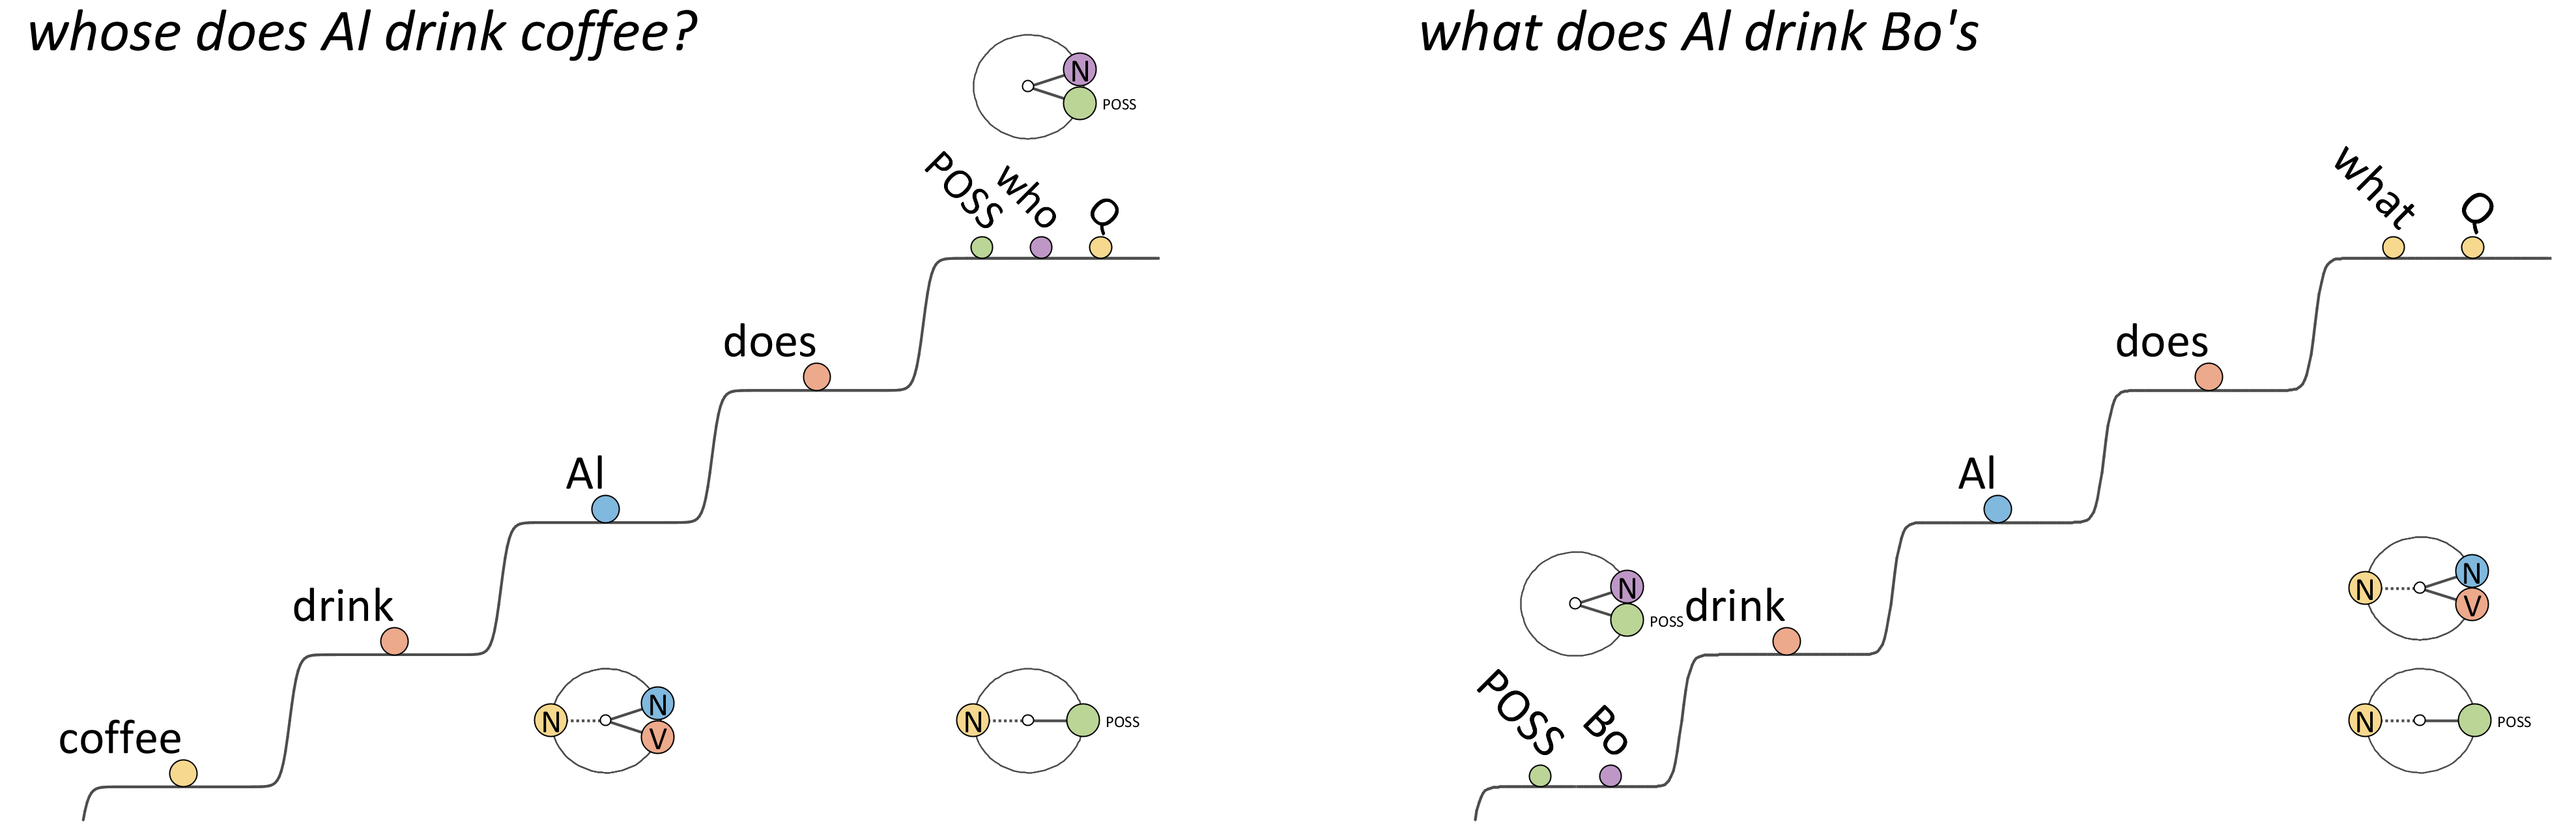
\includegraphics[width=\textwidth]{figures/Tilsen-img166.png}
\caption{\missingcaption}
\label{fig:7:22}
\end{figure}
 

  On the basis of the above patterns we can tentatively hypothesize \textit{a strong coupling constraint} on question promotion. This constraint holds that systems which are relatively strongly coupled—here defined in an ad-hoc manner as modifier-noun systems such as \{ADJ\}\{N\} and \{N\}\{POSS\}\{N\}—should be promoted together. This is admittedly problematic because it is not well motivated from a microscopic perspective, and does not seem to fall out naturally from the basic concepts of our theory. The strong coupling constraint on promotion does nonetheless seem to hold in other contexts, such as topicalization, and may be applicable for constituency intuitions more generally. The coherence of (a) and non-coherence of (b) and (c) can be understood in this way:

  \ea
  \ea[]{Cold coffee, Al drinks.}
  \ex[*]{Cold, Al drinks coffee.}
  \ex[*]{Coffee, Al drinks cold}  (${\neq}$ Al drinks cold coffee)
  \z
  \z
  
  There are many cases in the literature of exceptions to extraction from islands. These “exceptions” have a straightforward interpretation in the o/el framework, and indeed, the occurrence of exceptions is a basic prediction of the o/el account. Specifically, once we recognize that islands arise from grounding reorganizations and that surroundings forces can act to maintain systems in an excited state, it is expected that states which would otherwise be non-coherent can be coherent when there are factors which work toward that end. For example, consider the extraction from a relative clause in \REF{ex:7:1a} (cf. \citep{Erteschik-ShirLappin1979}) and the extraction from a finite clause adjunct in \REF{ex:7:1b} (cf. \citep{Truswell2011}):

\ea  \label{ex:7:1}
 \ea{\label{ex:7:1a} This is the kind of coffee that there are many people who like.}
 \ex{\label{ex:7:1b} This is the coffee that I got sick when I drank.}
\z
\z

\ea \label{ex:7:2}
\ea[*]{\label{ex:7:2a}Al drank coffee many people who like.}
\ex[*]{\label{ex:7:2b}Al drank coffee when I drank.}
\z
\z

\ea \label{ex:7:3}
  \ea[?]{Al drank coffee that there are many people who like.}
  \ex[?]{Al drank coffee that I got sick when I drank.}
\z
\z

In \REF{ex:7:1a} the [coffee]\{N\} system should be grounded by the reorganization associated with the wh-relative clause (cf. \ref{ex:7:2a}), and in \REF{ex:7:1b} it should be grounded by the reorganization associated with the adverbial clause (cf. \ref{ex:7:2b}). There are a couple aspects of the exceptional examples in \REF{ex:7:1} which are noteworthy. First, a non-grounding reorganization associated with a \textit{that} complement clause follows the excitation of [coffee]\{N\} and precedes the relevant grounding reorganization. Second, the [coffee]\{N\} system occurs in a cleft configuration (\textit{this is the coffee}) in the \REF{ex:7:1} examples, which contrast with parallel examples in \REF{ex:7:3} that have a reduced propensity for coherence. Third, there is not a competing \{-N\} system in these examples. These three factors may be responsible for creating a circumstance in which [coffee]\{N\} can remain in a excited state through the grounding reorganization, or in which the system is only weakly grounded and can be re-excited to achieve coherence. Indeed, “pragmatic” mechanisms that appear to override grounding reorganizations can be reinterpreted as forces which drive an interpretation trajectory to reach a coherent state, doing so by exciting a recently grounded system which may be particularly susceptible to re-excitation.

In the above analyses of wh-patterns, we applied basic o/el configurational hypotheses in combination with hypothesized differences in grounding operations that occur with reorganization. So doing, we found that variation in the grounding propensities of various reorganizations—which were also useful for analyses of ellipsis and anaphora phenomena—also help us understand long-distance dependencies in wh question formation and island effects. As with ellipsis and anaphora, island pattern coherence intuitions can vary substantially (\citealt{Kluender1998,SprouseHornstein2013,SprouseEtAl2012}). For all three of these phenomena, we can understand the variation as the consequence of a tension between propensities to ground previously excited systems and mechanisms for maintaining systems in an excited state or ungrounding previously grounded systems. It is encouraging that the same concepts required for understanding ellipsis and anaphora provide a basis for analysis of many of the island patterns. This suggests that a comprehensive understanding of diverse syntactic phenomena is achievable.

